\subsection{Reconstruction and calibration}
\label{sec:rec}
 
The cell energy smaller than 0.5\mev is neglected in the clustering.
There are many different clustering algorithms to reconstruct the cluster for different kinds of calorimeters,
\eg Arbor, ML, APRIL, \etal \supercite{ruan2014arbor,Belayneh2019CalorimetryWD,Li:2020llf}. 
The main idea is to fully exploit the advantage of the shower characteristics for a given calorimeter. 
%As this is a preliminary simulation study, 
%many performance parameters are given value in this simulation study, 
%The current reconstruction method is a simle method, 
A simple but effective algorithm is used for preliminary analyses. 
The algorithm used this study is similar to the method used in the current \lhcb calorimeter with an extension to multi-layer configuration. 
It is simple and effective for preliminary analyses. 
In this algorithm, 
the seed cell for each layer (26 layers in total), 
which is used as a starting point for the aggregation, is first searched for according to the energy distribution.
The cell energies around the seed cell are then added for each layer.
Finally, these energies in all layers are summed to form a shower if they are in a similar position in the $x$-$y$ plane.


\subsubsection{Shower reconstruction}
The cluster layer energy is obtained by adding all cell's energy together:
\begin{equation}
E_{layer} = \sum_{i}^{cells}{E_i}
\end{equation}
and the layer cluster position are estimated: 
\begin{equation}
\begin{split}
x_{layer} = (\sum_{i}^{cells}{x_i \times E_i})/E_{layer} \\
y_{layer} = (\sum_{i}^{cells}{y_i \times E_i})/E_{layer} \\
z_{layer} = z_i
\end{split}
\end{equation}
As the thickness of silicon sensor is very small,
$4\mum$ here, 
the silicon sensor z position is taken as the layer cluster position.

The layer time is also obtained from the cell in the same layer:
\begin{equation}
T_{layer} = (\sum_{i}^{cells}{T_{i,cali} \times E_i})/E_{layer}
\end{equation}
considering the developing time of the shower,
usually, 
the measured time from the cells around seed cell is larger than the seed cell time,
therefore, 
the used time in the above formula is calibrated,
the calibration method will be addressed later.

The shower information is estimated from the each layer cluster calibrated,
with the layer energy weight.
In the current reconstruction algorithm,
the layer cluster energy smaller then 3\mev is overlooked, 
considering the random effect.


%We are also investigating other algorithms for the clustering and shower reconstruction, \eg APRIL developed by B. Li \etal for ILC\cite{Li:2020llf}. 
%Figure~\ref{fig:ReconstructedShowerpi0} shows an example of two showers reconstructed by the APRIL algorithm from the two photons decaying from a $10\gev$ $\piz$. 
%The reconstructed energies of the two photons are $2.58\gev$ and $7.20\gev$, and the energy-weighted centres of the two clusters are $(29.2, -10.2, 1256.8)\cm$ and $(-8.7, 3.2, 1257.2)\cm$ respectively.
%%%%%%%%%%%%%%%%%%%%%%%%%%%%%%%%%%%%%%%%
%\begin{figure}[tb]
%  \begin{center}
%    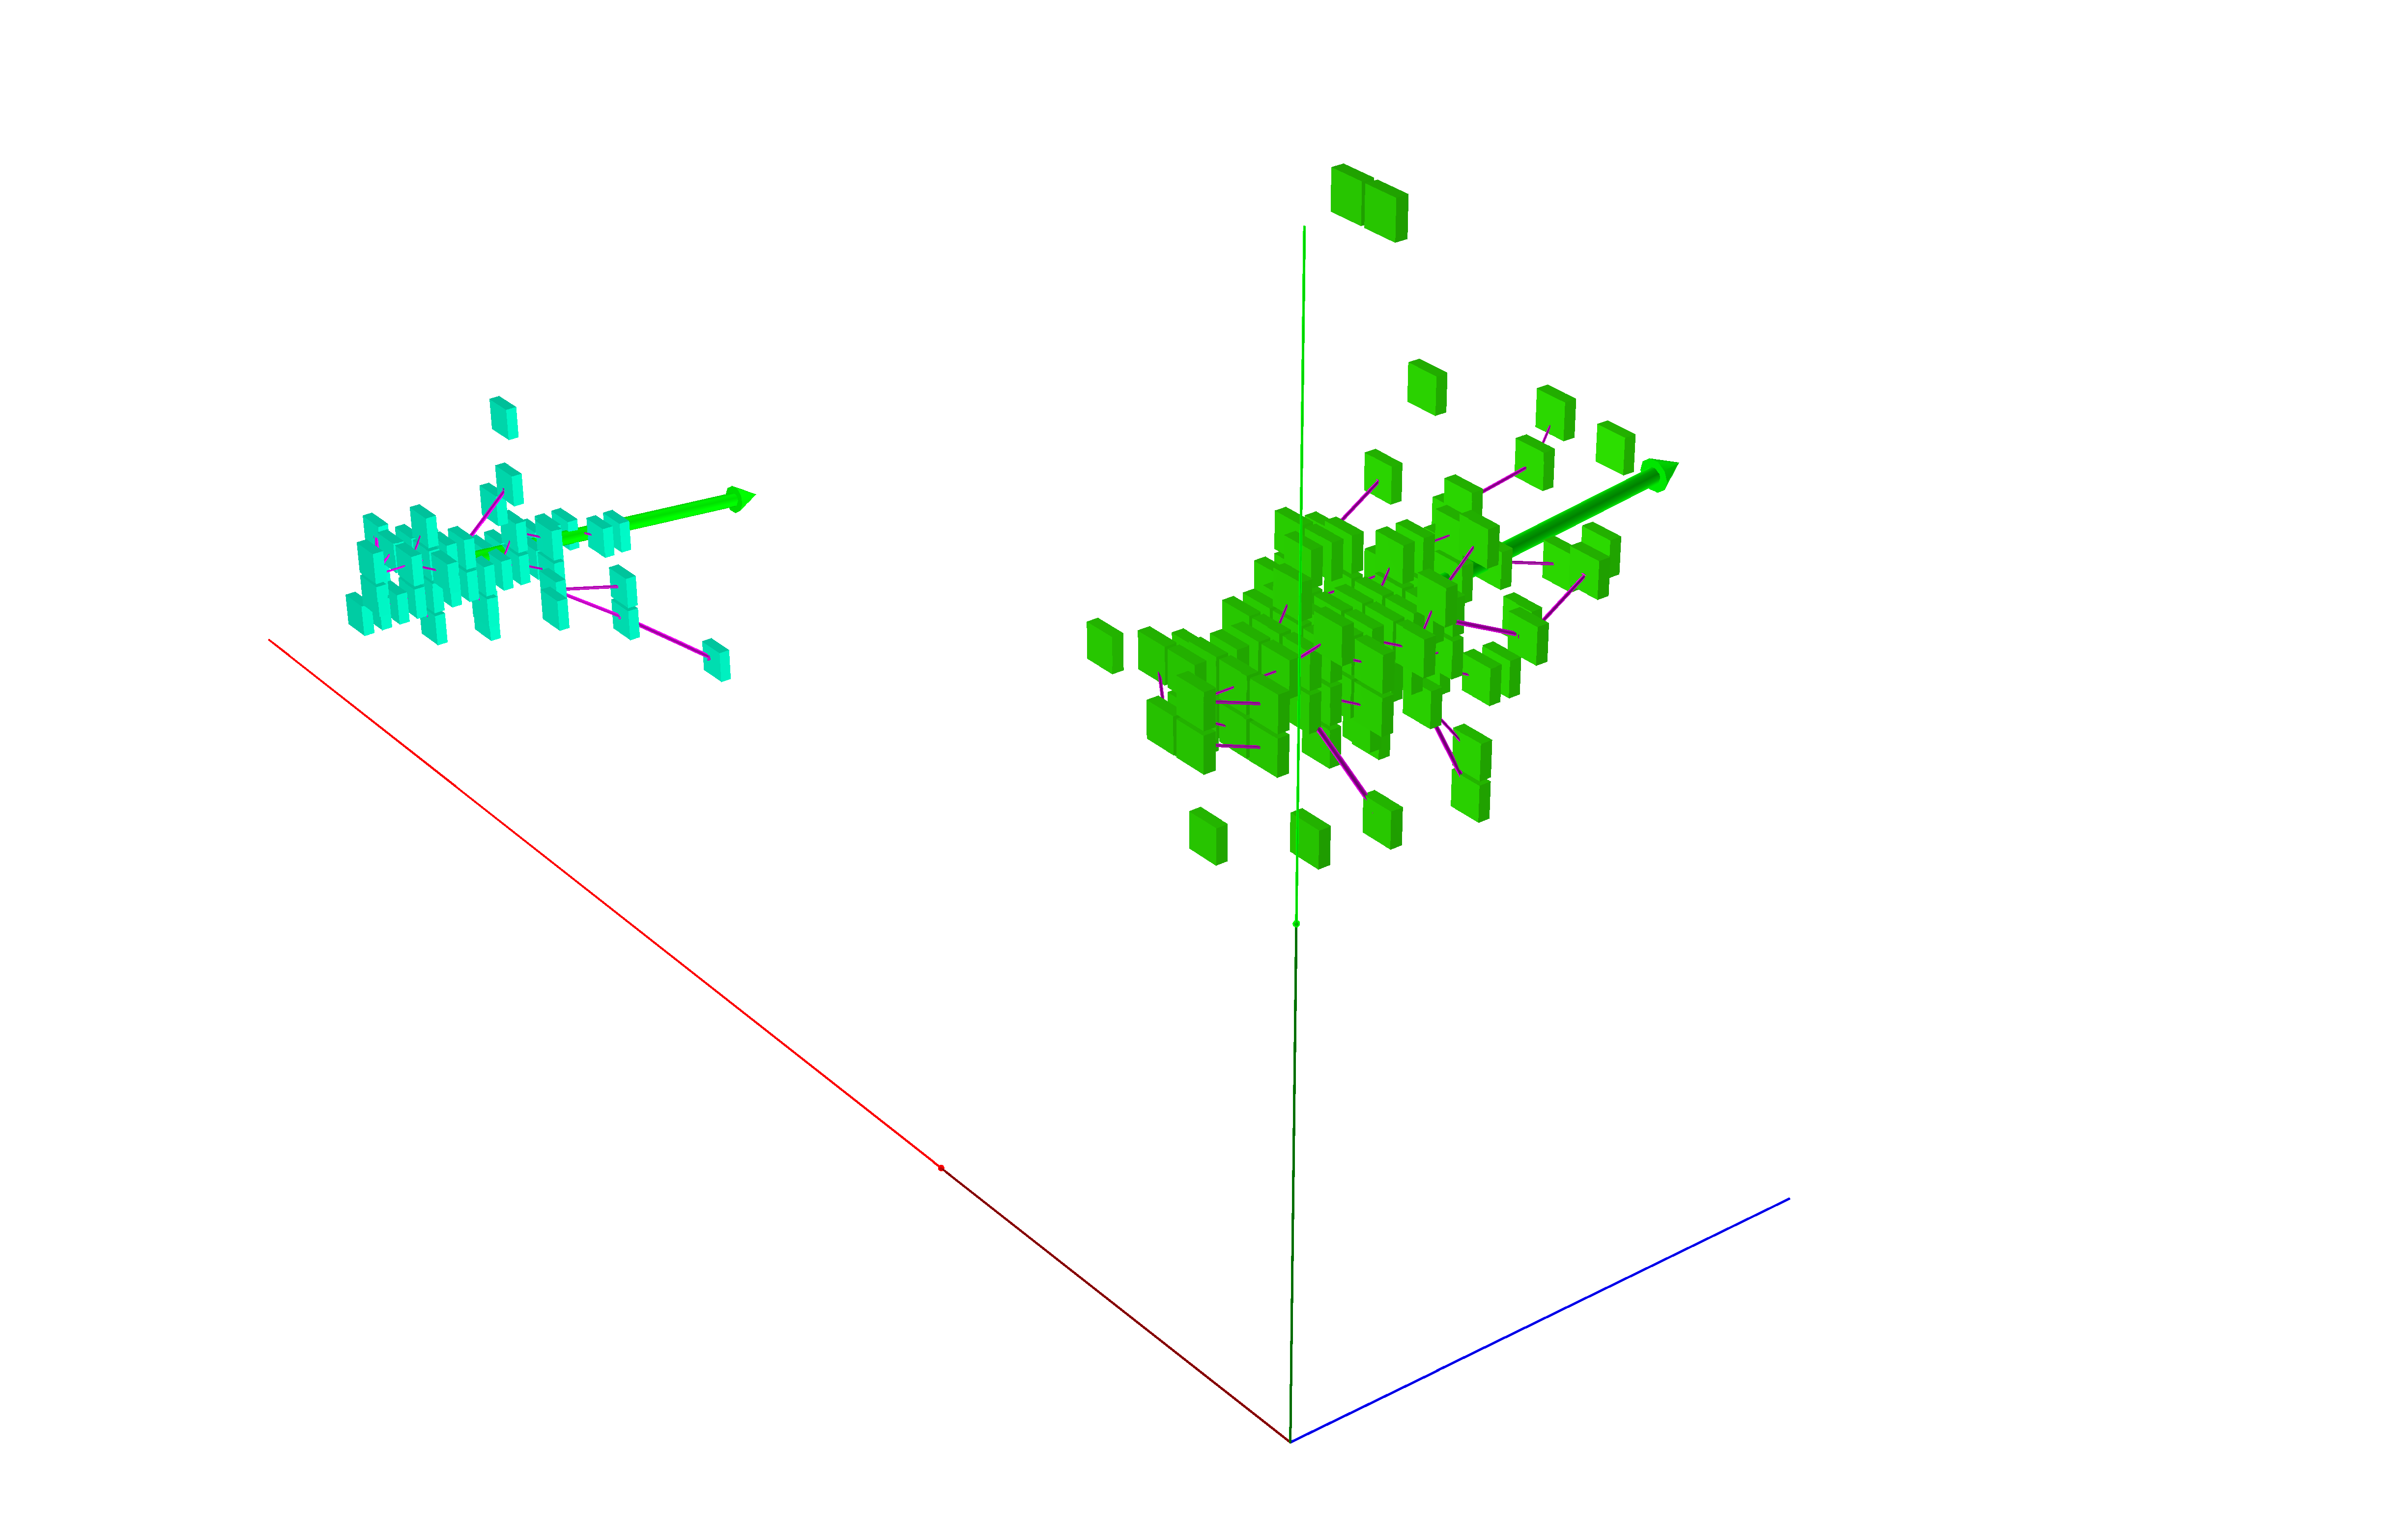
\includegraphics[width=0.60\linewidth]{figs/Reconstructed_showers.pdf}
%    \vspace*{-0.5cm}
%    \end{center}
%    \caption{
%    %\small %captions should be a little bit smaller than main text
%     Reconstructed showers of two photons from a $\piz\to\gamma\gamma$ decay. The mother $\piz$ kinetic energy is $10\gev$, and the reconstructed photon energies are $2.58\gev$ and $7.20\gev$. 
%  }
%  \label{fig:ReconstructedShowerpi0}
%\end{figure}
%%%%%%%%%%%%%%%%%%%%%%%%%%%%%%%%%%%%%%%


%\subsection{Calibration and Resolution}
%This is an interesting part, especially to the layer cluster time calibration.

\subsubsection{Energy calibration}
The method to calibrate the reconstruct shower energy is similar to the previous study,
by a lineaer function:
\begin{equation}
E_{cali} = \alpha \times E_{rec} + \beta
\end{equation}
In the real experiment, 
the calibrated parameters are obtained from beam test or real running,
we estimate these numbers in from particle gun simulation here.
From the $\gamma$ event, 
we get the relation between the true particle energy and the reconstructed one,
as shown in Figure~.\ref{fig:energy_rela},
and fitted by a linear function.
The obtained values will be taken as the calibration parameters. 
After the calibration is finished, 
the energy resolution is studied, 
%as well as the performance with different injection angle, 
as shown in Figure.~\ref{fig:energy_res},
where the thicknesses of silicon is $4\mm$.

\begin{figure}[!thbp]
\centering
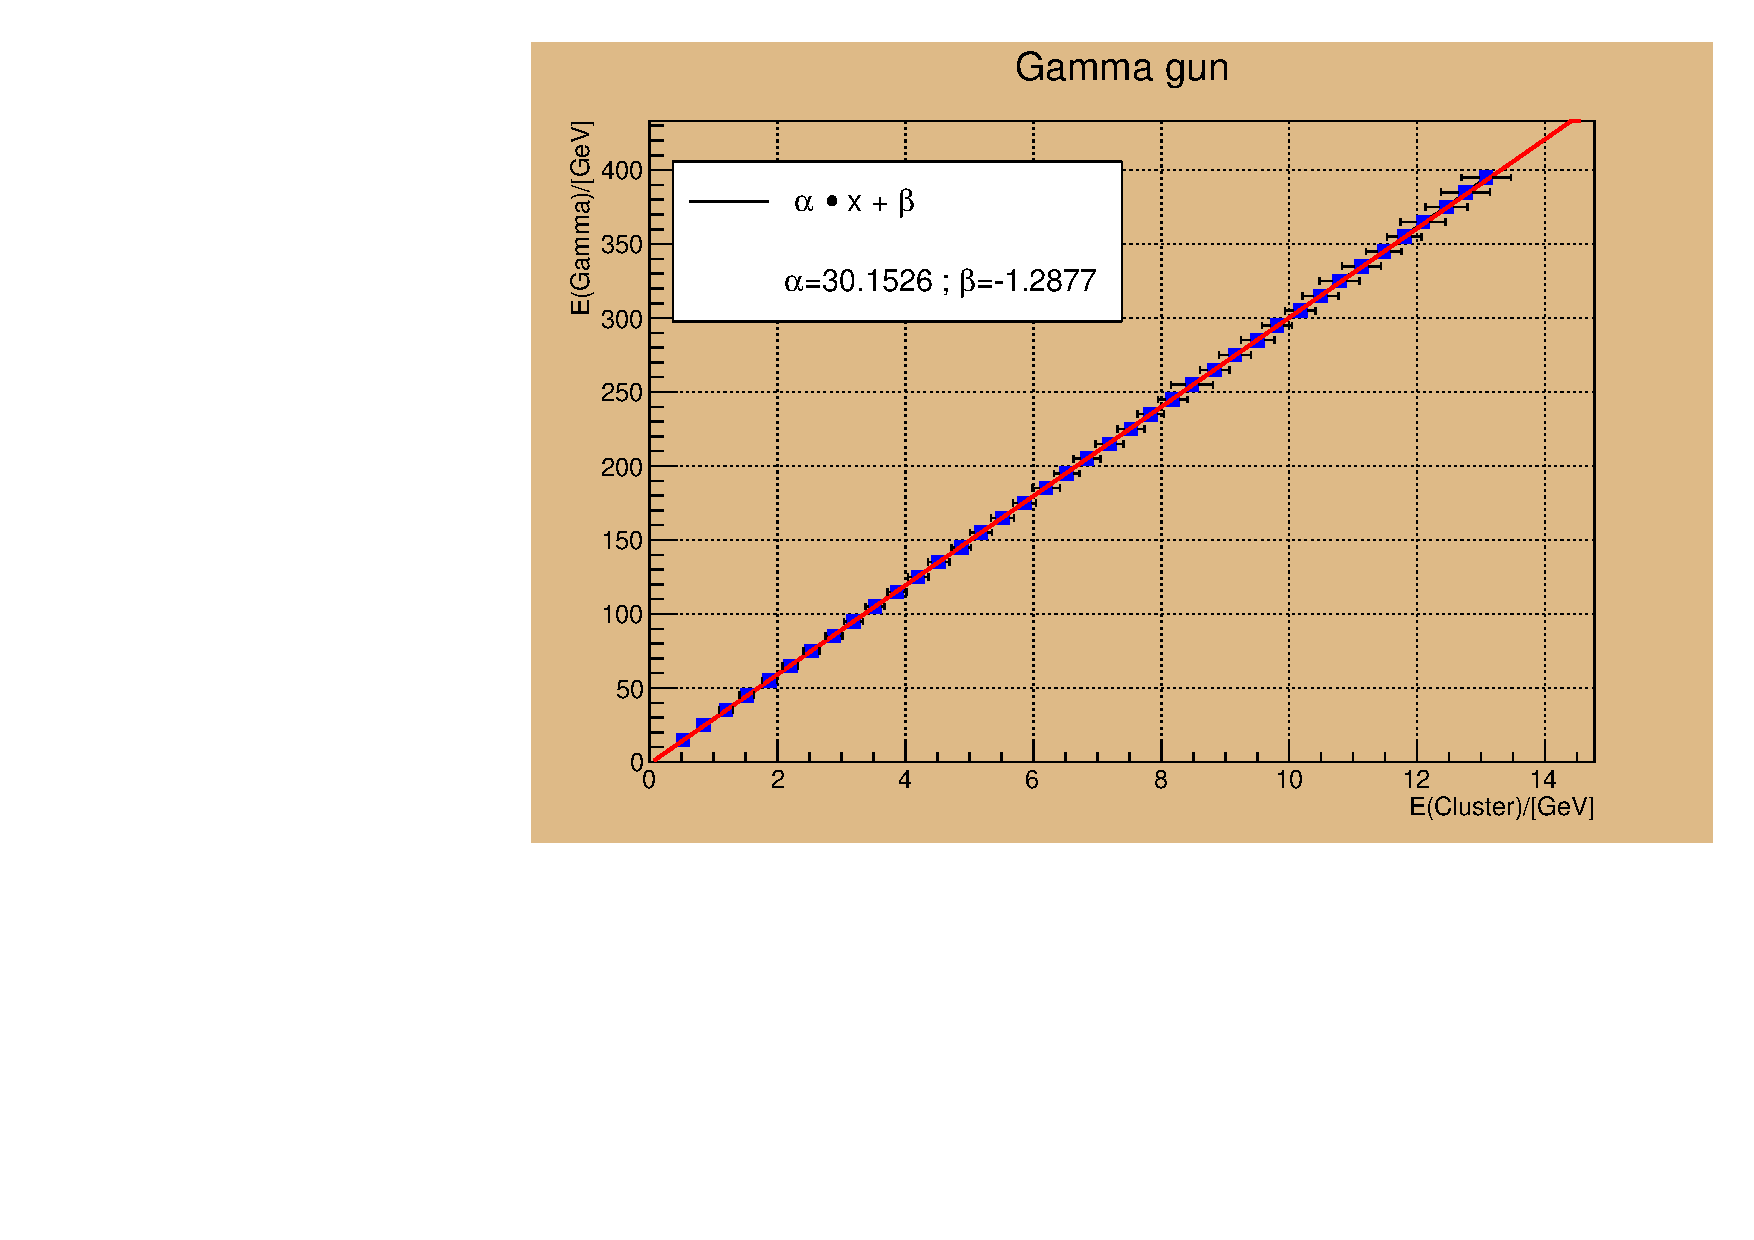
\includegraphics[width=0.55\textwidth]{Figures/06_ECAL/energy_res_rela_angle/rela.pdf}
\caption{The relation between particle true energy and reconstructed cluster shower energy.} 
\label{fig:energy_rela}
\end{figure}


\begin{figure}[!thbp]
\centering
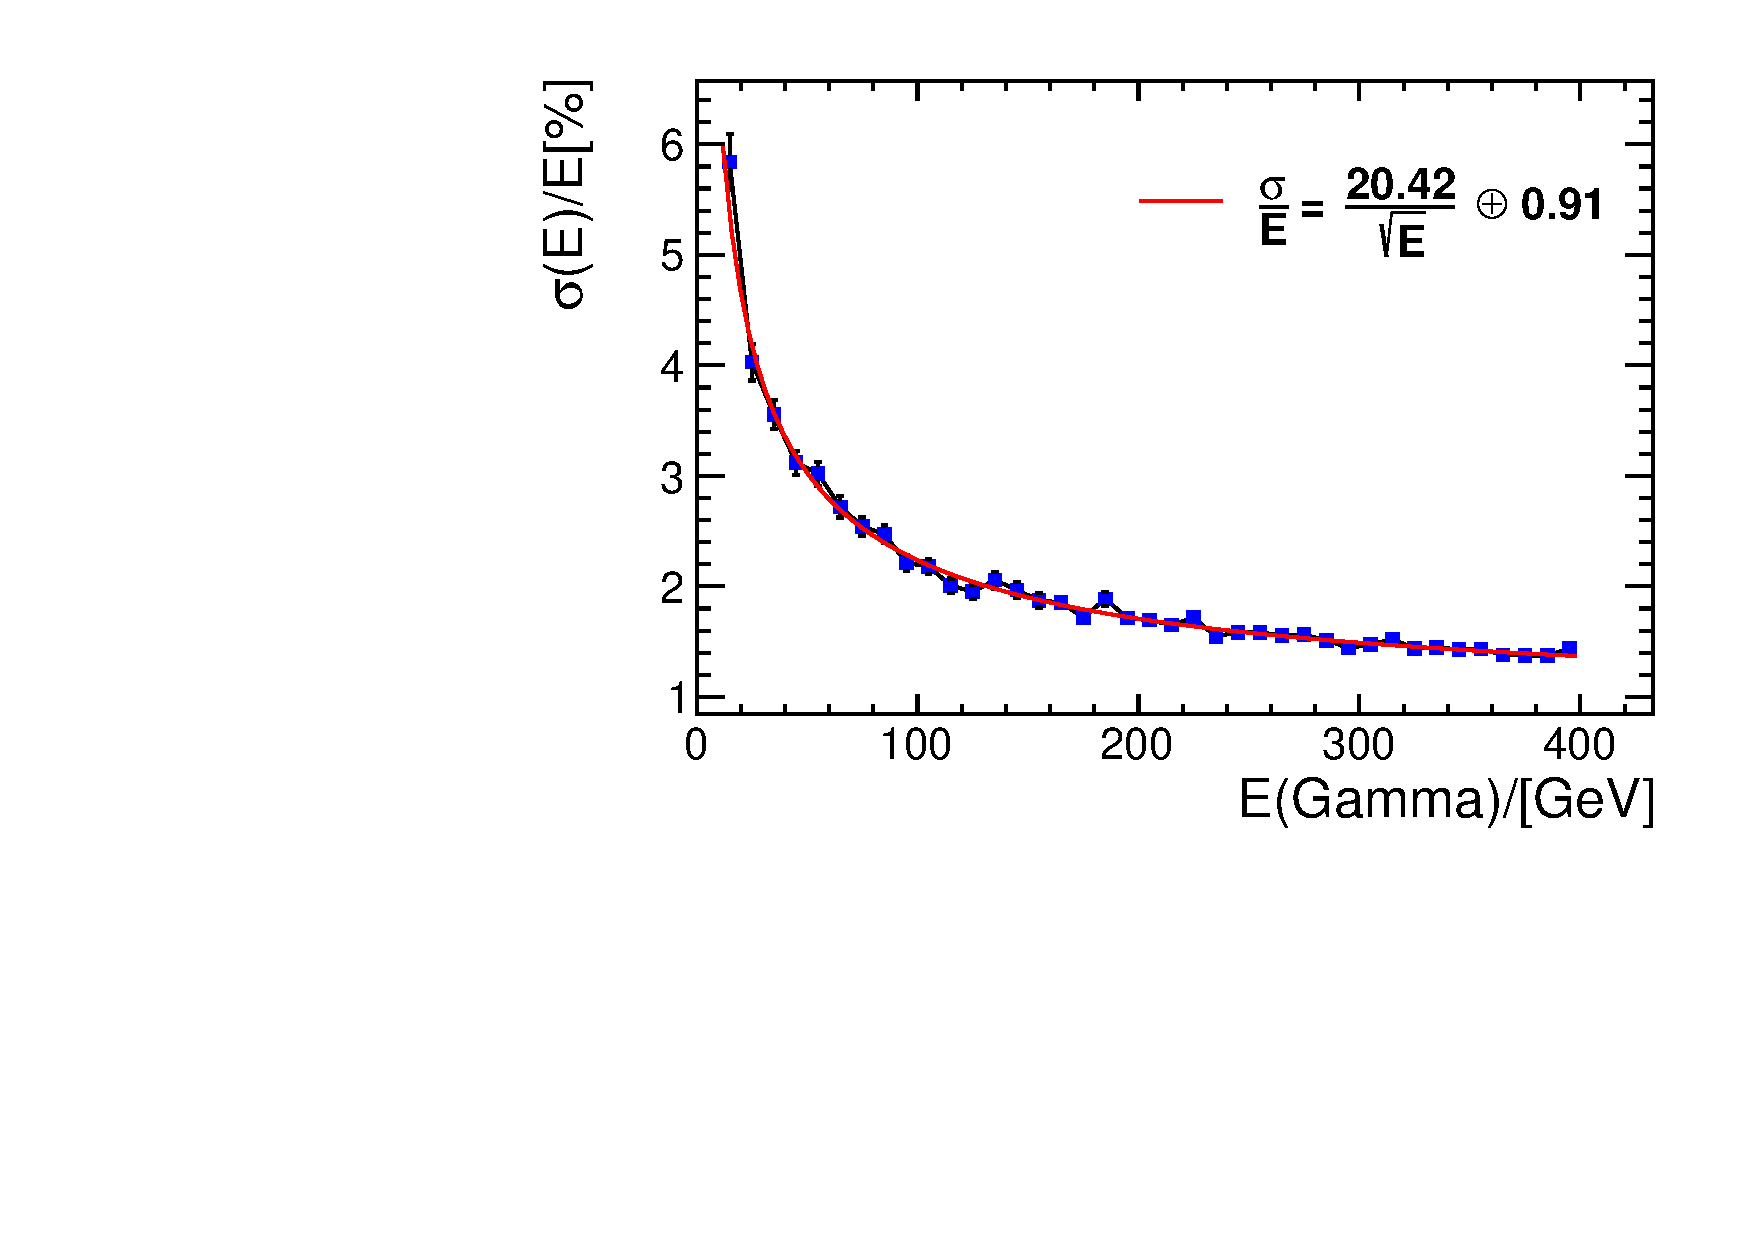
\includegraphics[width=0.48\textwidth]{Figures/06_ECAL/energy_res_rela_angle/res.pdf}
\put(-130,100) {\textrm{\small \bf(a)}}
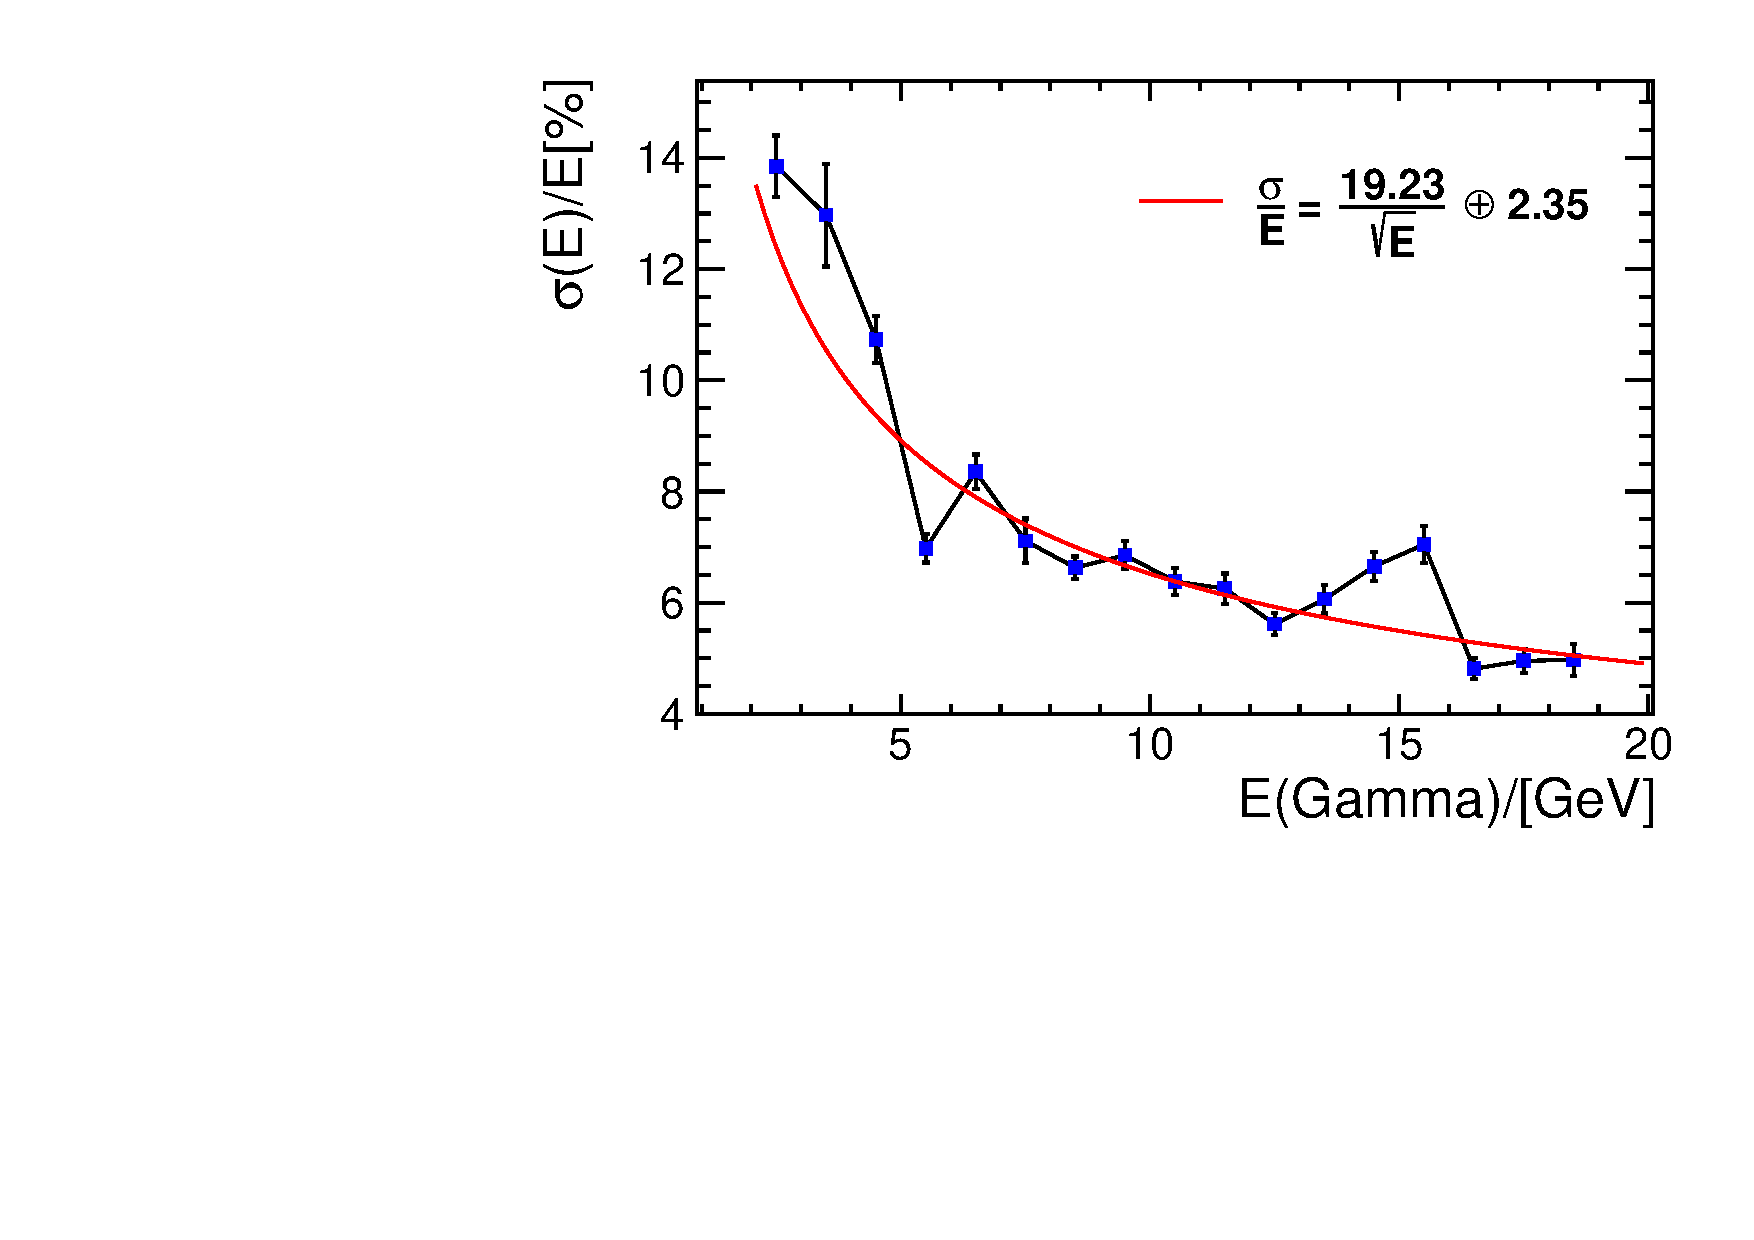
\includegraphics[width=0.48\textwidth]{Figures/06_ECAL/energy_res_rela_angle/res_small_energy.pdf}
\put(-130,100) {\textrm{\small \bf(b)}}\\
\caption{The energy resolution in different particle energy regions.} 
\label{fig:energy_res}
\end{figure}
%The Figure.(a) presents the resolution varies with the energy, while Figure.(bcd) show the performance with different $\gamma$ different incident angles.
%From this plots, we find that the resolution is much related to the deposited energy, but not the incident angle of particle at the \lhcb acceptance.


%\begin{figure}[!thbp]
%\centering
%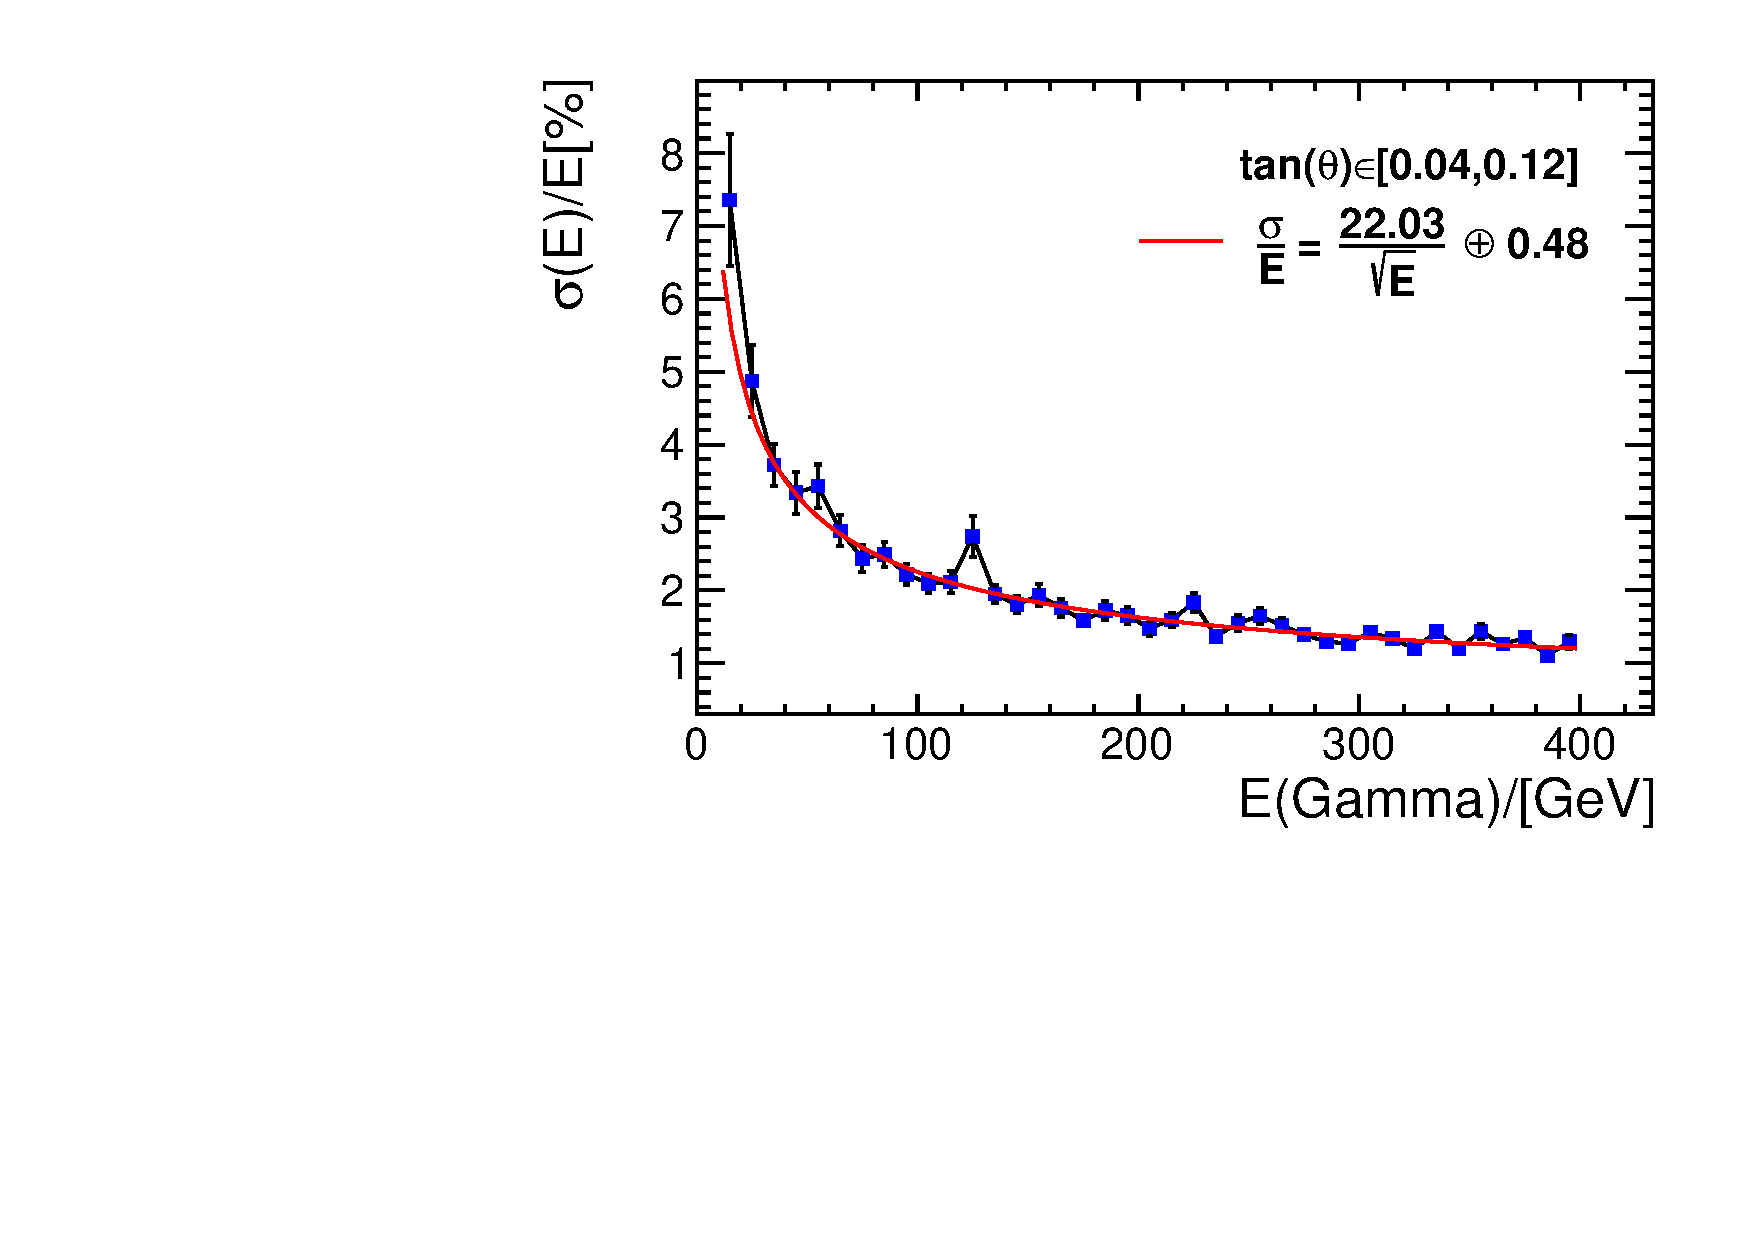
\includegraphics[width=0.45\textwidth]{Figures/06_ECAL/energy_res_rela_angle/res_angle1.pdf}
%\put(-130,100) {\textrm{\small \bf(a)}}
%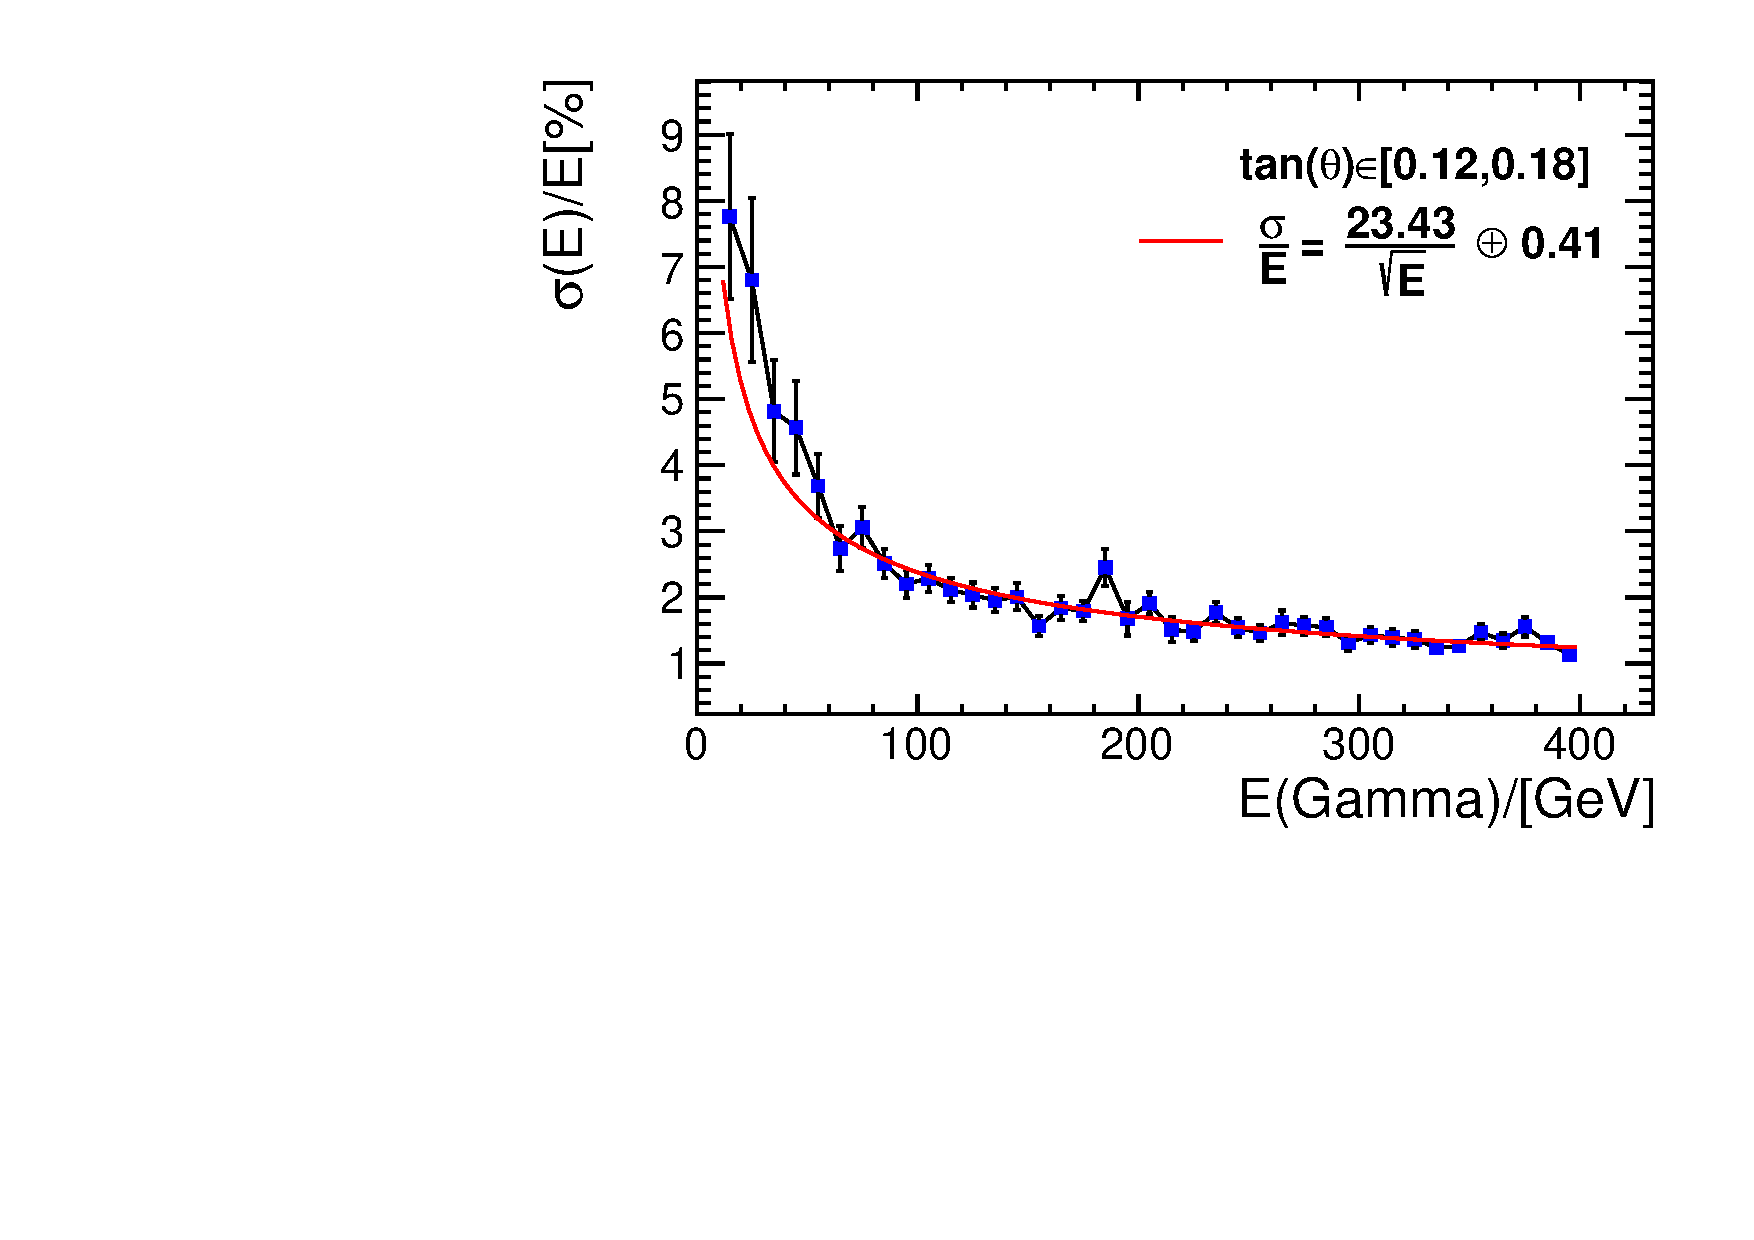
\includegraphics[width=0.45\textwidth]{Figures/06_ECAL/energy_res_rela_angle/res_angle2.pdf} 
%\put(-130,100) {\textrm{\small \bf(b)}} \\
%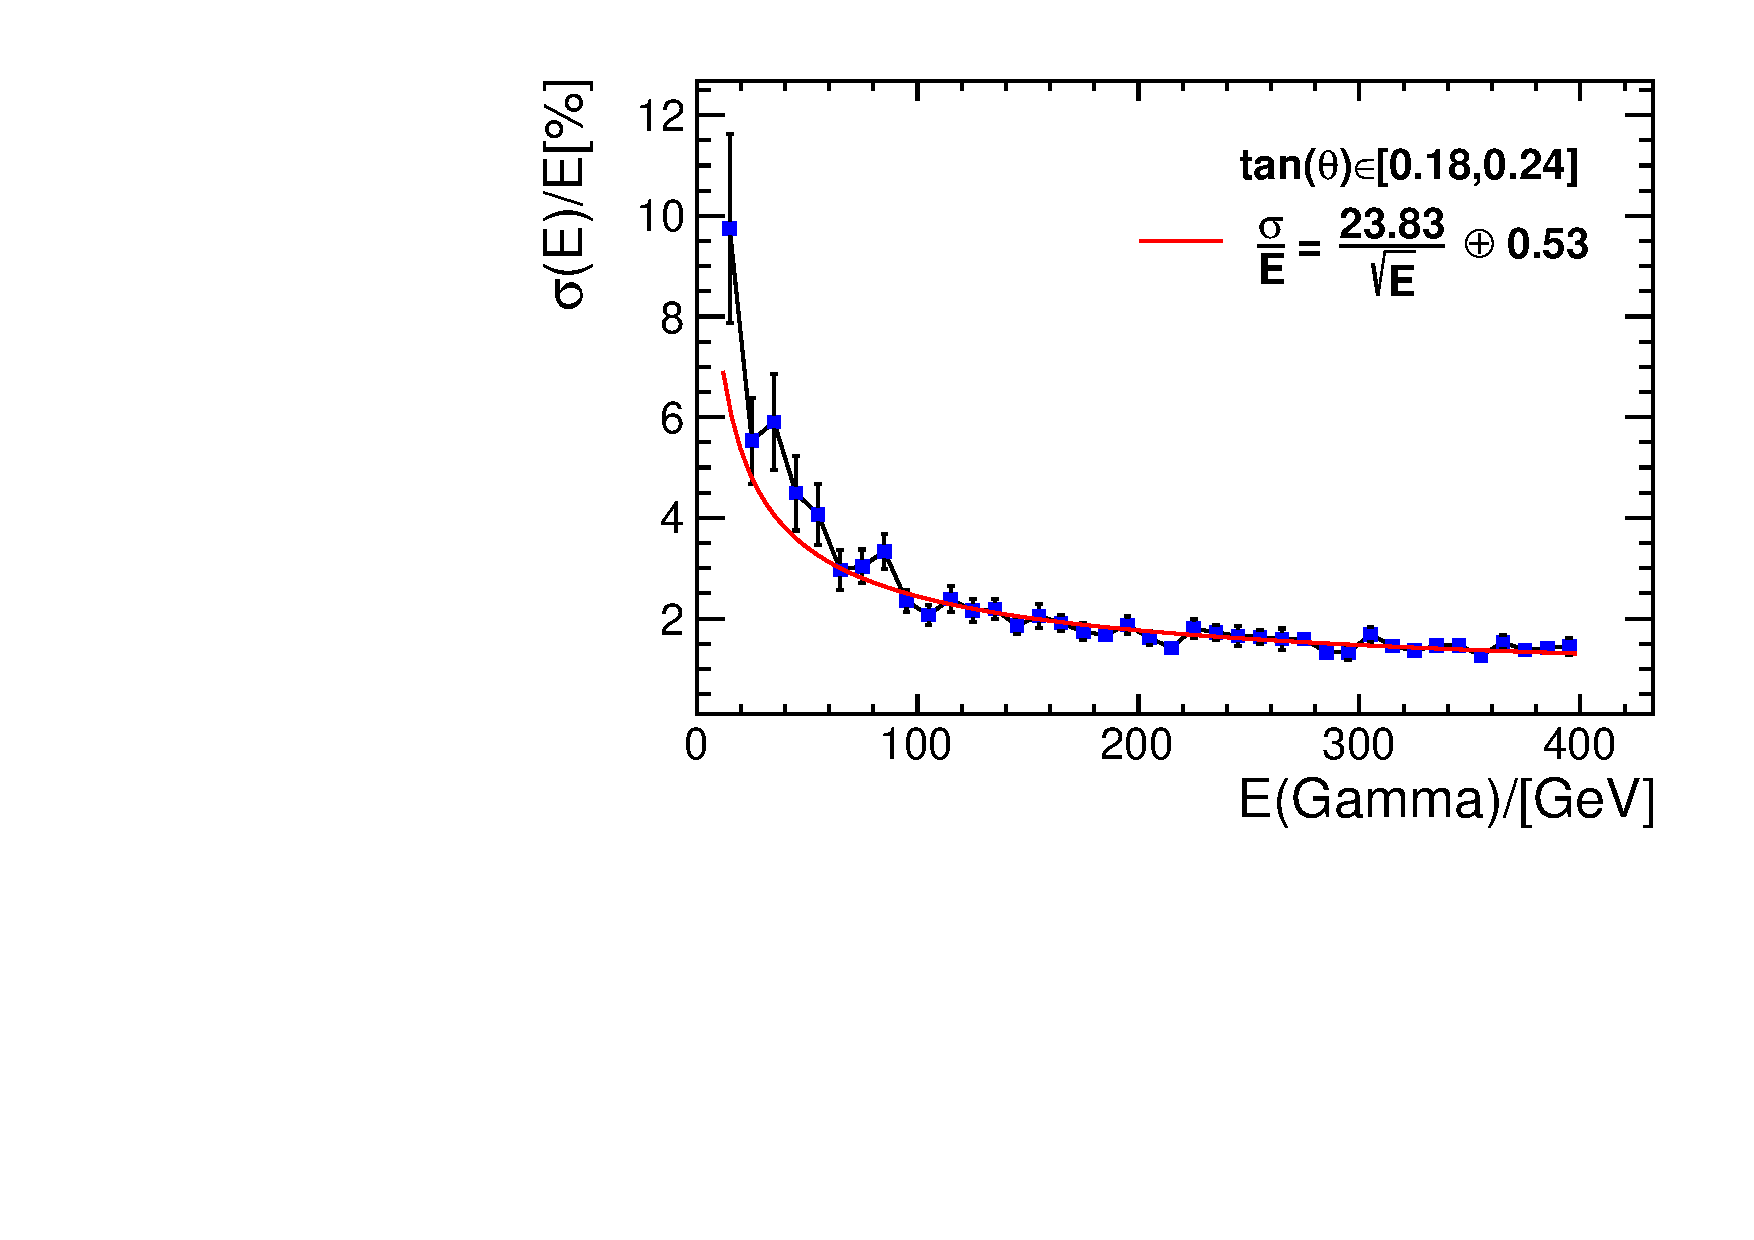
\includegraphics[width=0.45\textwidth]{Figures/06_ECAL/energy_res_rela_angle/res_angle3.pdf}
%\put(-130,100) {\textrm{\small \bf(c)}}
%\caption{The energy resolution with different incident particle angle.} 
%\label{fig:energy_res_angle}
%\end{figure}


The seed cell energy fraction in one layer cluster for each layer is shown in left of Figure.~\ref{fig:energy_E_seed}, 
according to this plot, 
we know that most of shower energy deposit in the seed cell, 
which is also the reason why we use current method to cluster.
Besides, the seed energy fraction becomes smaller as the shower development.

\begin{figure}[!tbp]
\centering
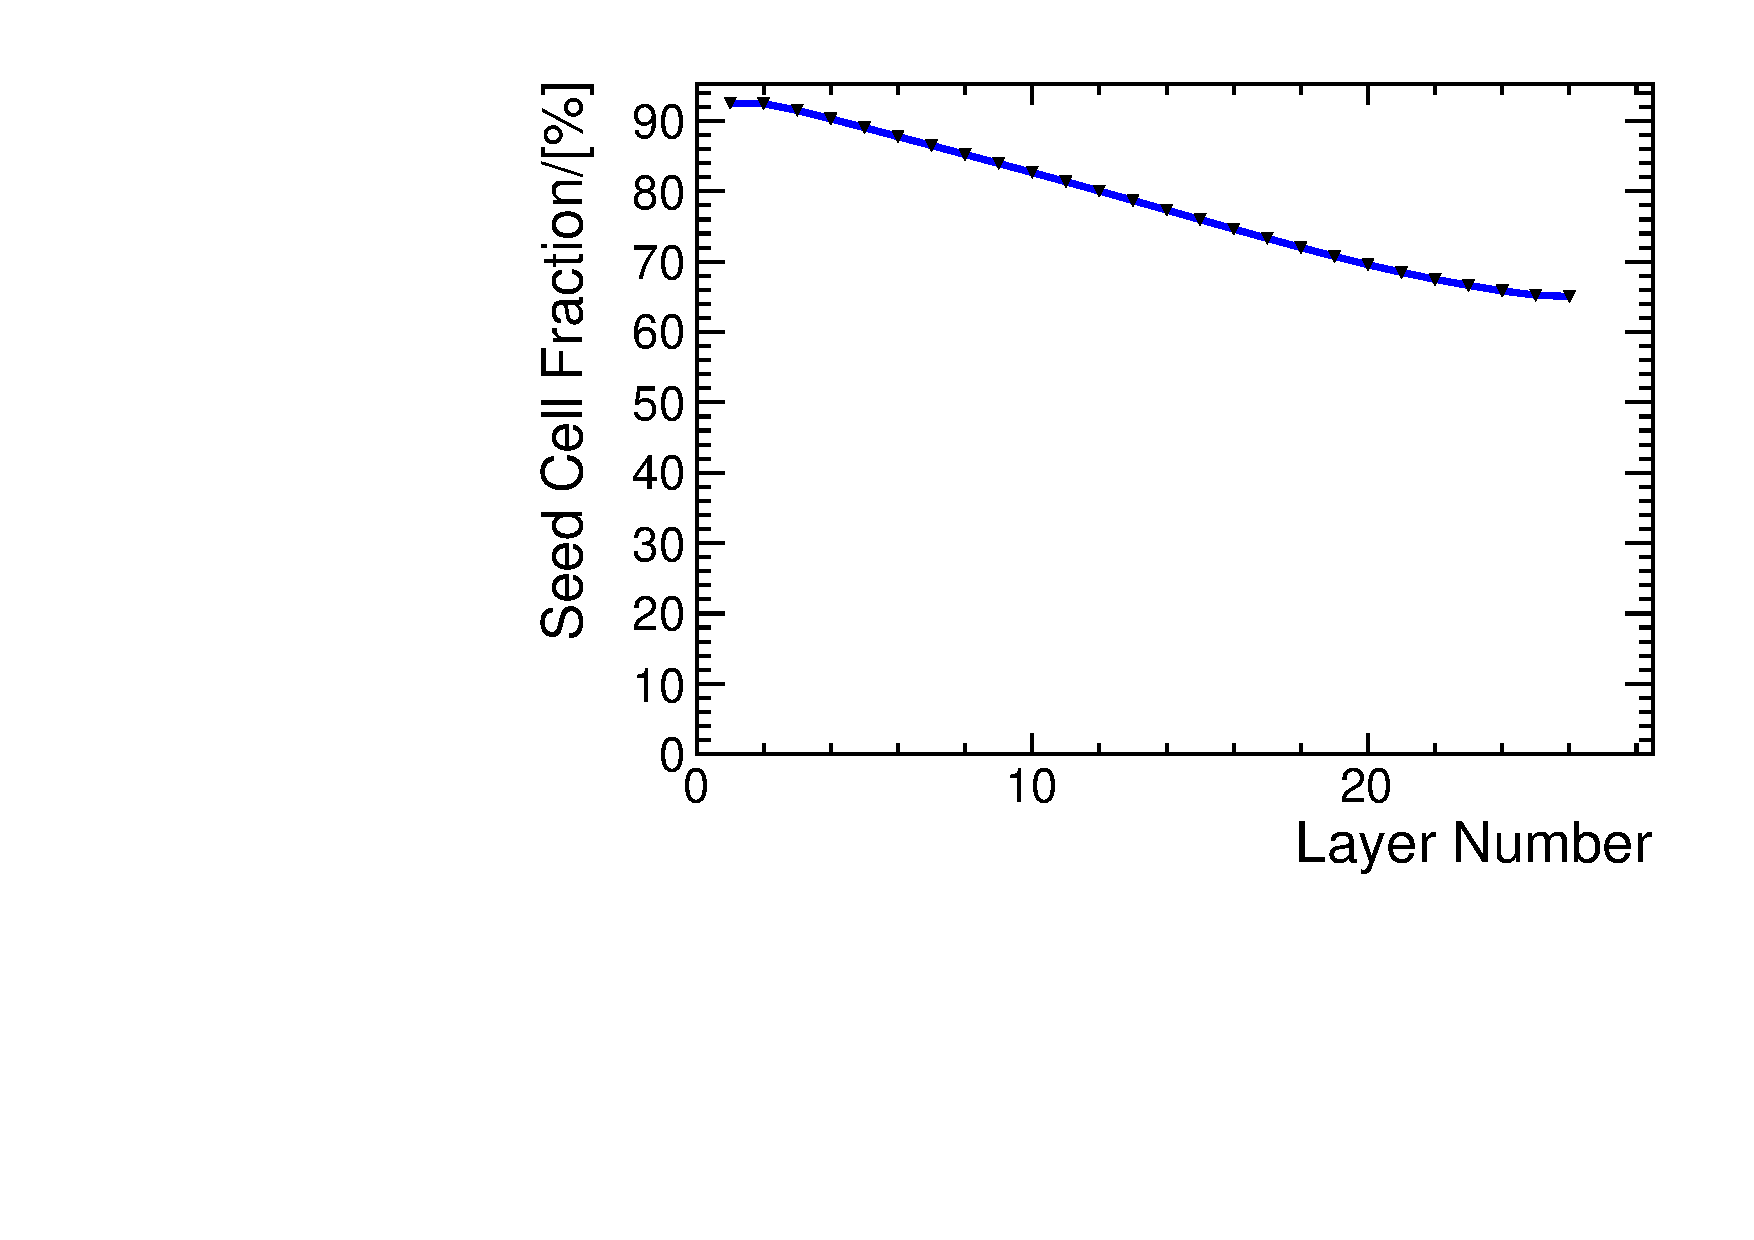
\includegraphics[width=0.48\textwidth]{Figures/06_ECAL/energy_res_rela_angle/E_fraction_each_layers.pdf}
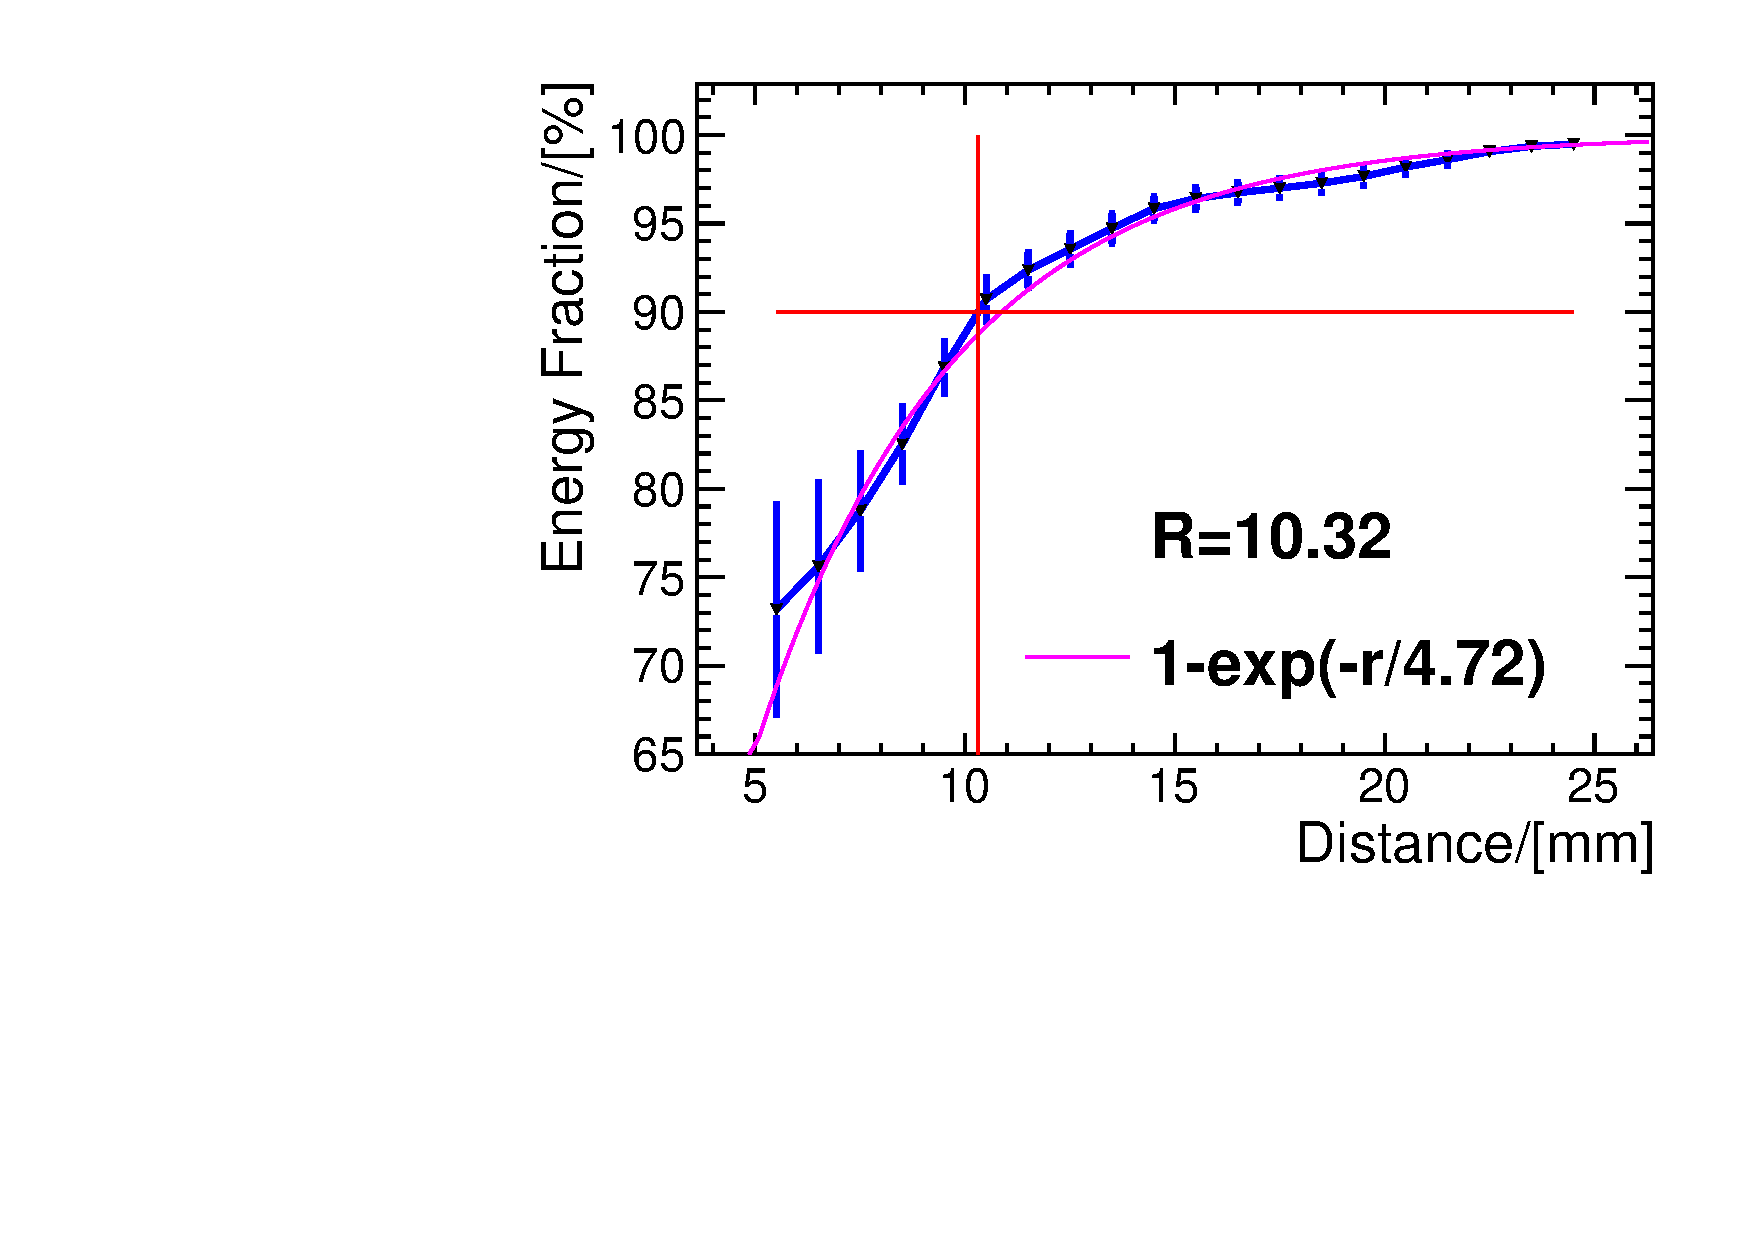
\includegraphics[width=0.48\textwidth]{Figures/06_ECAL/energy_res_rela_angle/E_moliere.pdf}
   \caption{The seed cell energy fraction for each layer (left).
   The estimated Moliere radius (right).} 
\label{fig:energy_E_seed}
\end{figure}

A check to the Moliere redius is also performed, as shown in right of Figure.~\ref{fig:energy_E_seed}, 
which is obtained from the reconstructed shown energy from the silicon sensors.
The estimated Moliere radius is around $10.3\mm$, which is a litter larger than the value of tungsten from PDG as the silicon and gap in the current Multi-layer Si-W \ecal model.
Besides, 
this plots also shows the lateral development of shower in Si-W \ecal,
the  distribution is parameterized by this function:
\begin{equation}
f = 100(1-e^{r/A})
\end{equation}
where $r$ is the cell distance to the shower energy baryon axis, 
$A=4.73$ is obtained from fitting, 
which is a free parameters.:q
Actually, 
the relations between energy fraction and distance in each layers are little different,
not go too far into this in the preliminary study.

%\begin{figure}[!tbp]
%\centering
%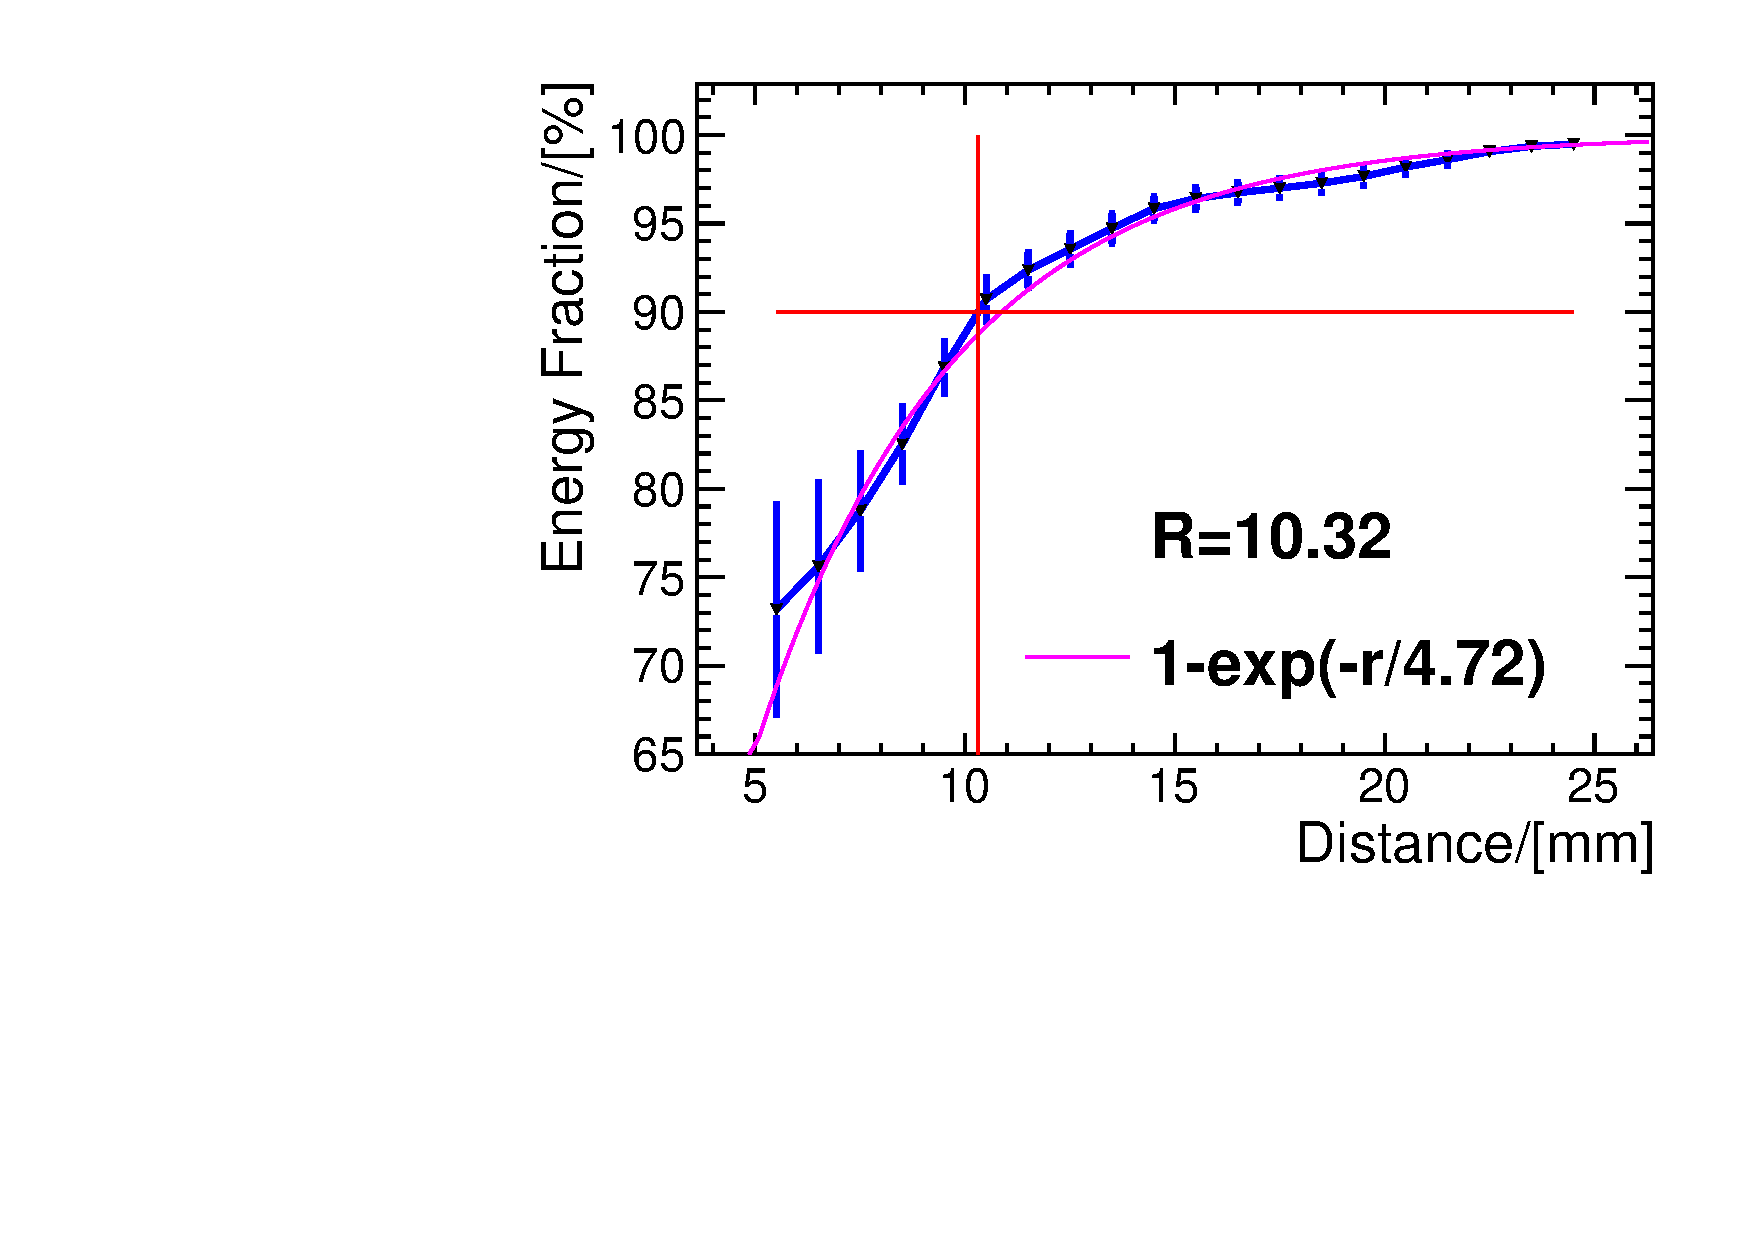
\includegraphics[width=0.5\textwidth]{Figures/06_ECAL/energy_res_rela_angle/E_moliere.pdf}
%\caption{The estimated Moliere radius.} 
%\label{fig:energy_E_moliere}
%\end{figure}

Figure~\ref{fig:energyresolutionSiW} shows the energy resolution as a function of the incident electron energy for different thicknesses of the silicon layers with the cell size of $1.0\times1.0\cm^2$ and the thickness of $3.5\mm$ for the tungsten layers. 
It shows that the energy resolution improves as the Si thickness increases. 
The dependence of the energy resolution on the cell size of the silicon layer and the thickness of the tungsten layer is almost negligible.
The energy resolution is around $15\%$ ($5\%$) when the energy of the electron is $1\gev$ ($10\gev$).
%%%%%%%%%%%%%%%%%%%%%%%%%%%%%%%%%%%%%%%%
\begin{figure}[tb]
  \begin{center}
    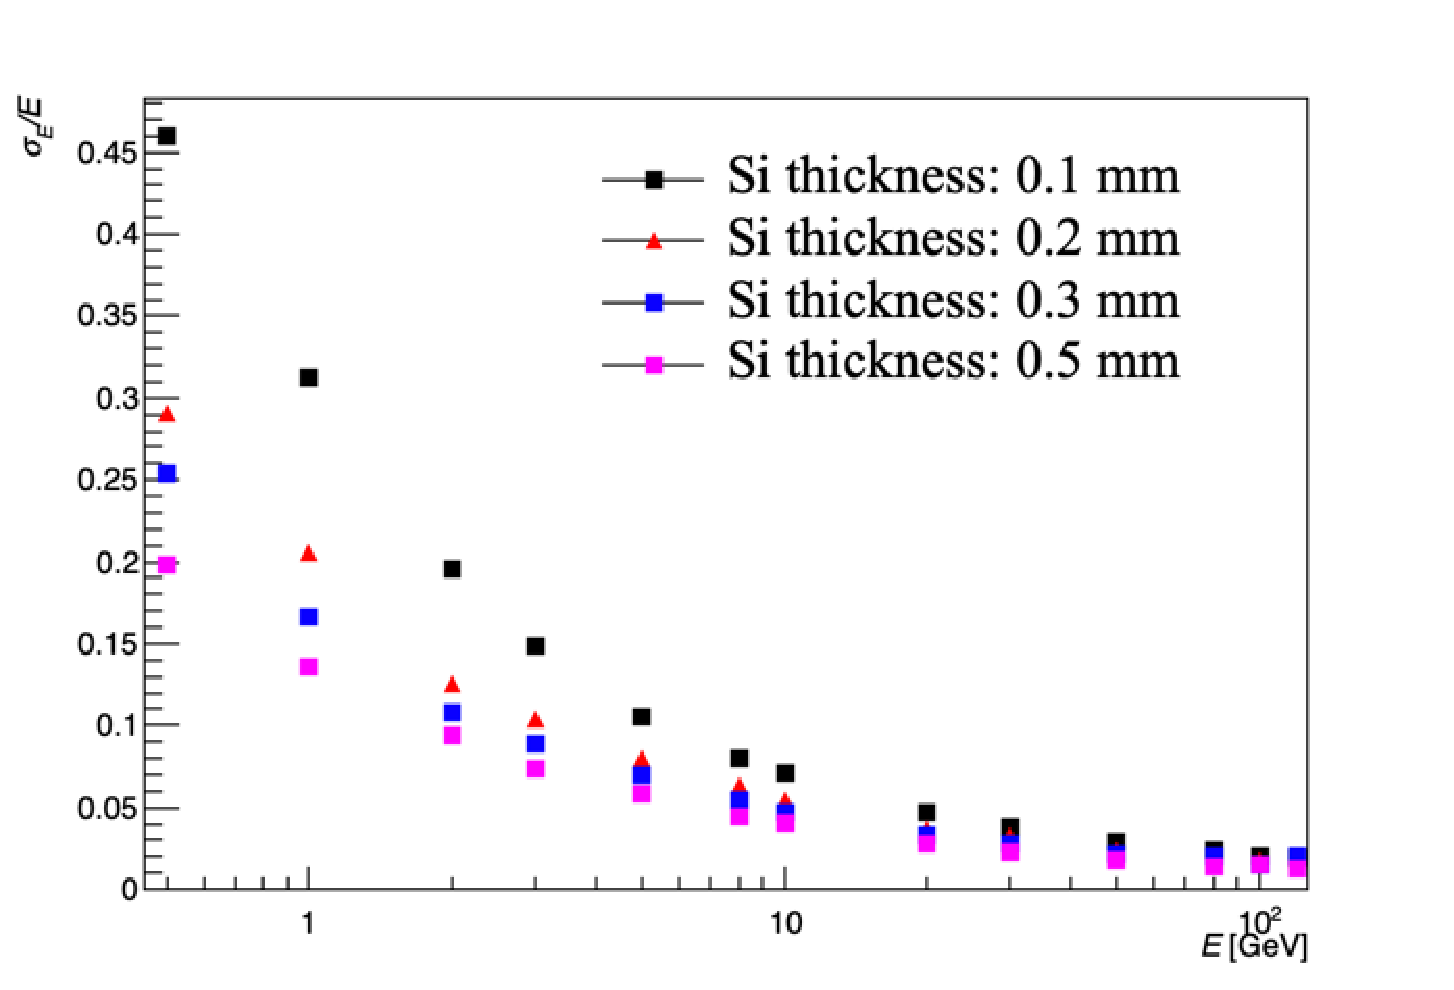
\includegraphics[width=0.6\linewidth]{Figures/06_ECAL/plotsZW/resolutionE_compare_Siwidth_1x1.pdf}%\put(-32,133){(a)}
    \vspace*{-0.5cm}
  \end{center}
  \caption{
  Energy resolution of electron showers as a function of the incident electron energy for different thicknesses of the silicon layers. 
   The cell size is $1.0\times1.0\cm^2$ and the thickness of the tungsten layers is $3.5\mm$.
  }
  \label{fig:energyresolutionSiW}
\end{figure}
%%%%%%%%%%%%%%%%%%%%%%%%%%%%%%%%%%%%%%%%


\subsubsection{Position calibration}

The method to calibrate the layer cluster position is similar to the one used in current \ecal.
And the position calibration is performed according to the relative position in one cell.
As shown in the left of Figure.~\ref{fig:position_rela},
the reconstructed position is not exactly equal to the true position,
the relation of these values is estimated by Function.~\ref{eq:pos_cali}, also used in parameterized simulation.
%\begin{equation}
%x_{true} = f \times b \times asinh(\frac{x_{rec}}{\Delta}cosh\frac{\Delta}{b})
%\end{equation}
the left plot of Figure.~\ref{fig:position_rela} is a example to the 15th layer, 
actually, 
every layer is studied separately, 
as shower shape changes with depth of the incident.

\begin{figure}[!tbp]
\centering
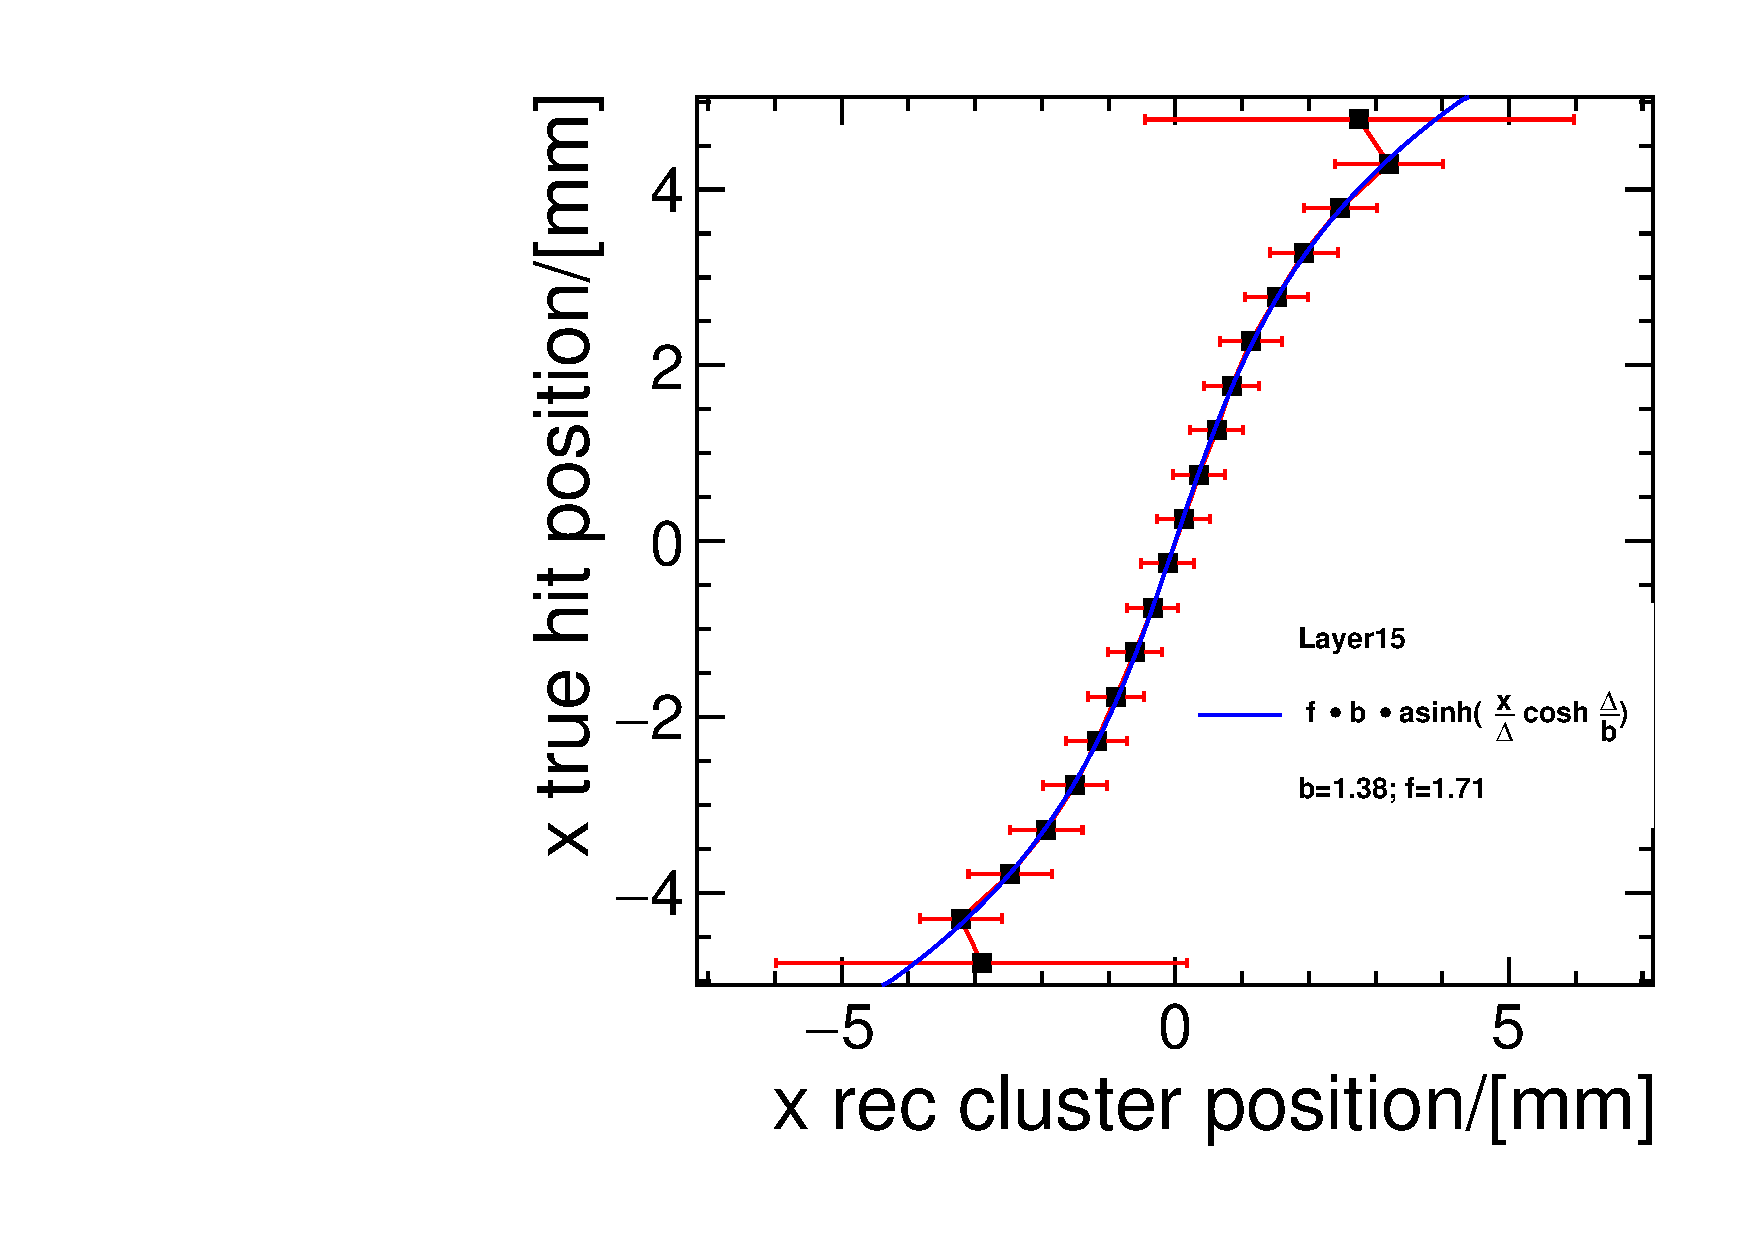
\includegraphics[width=0.45\textwidth]{Figures/06_ECAL/position_res_cali/pos_cali_15.pdf}
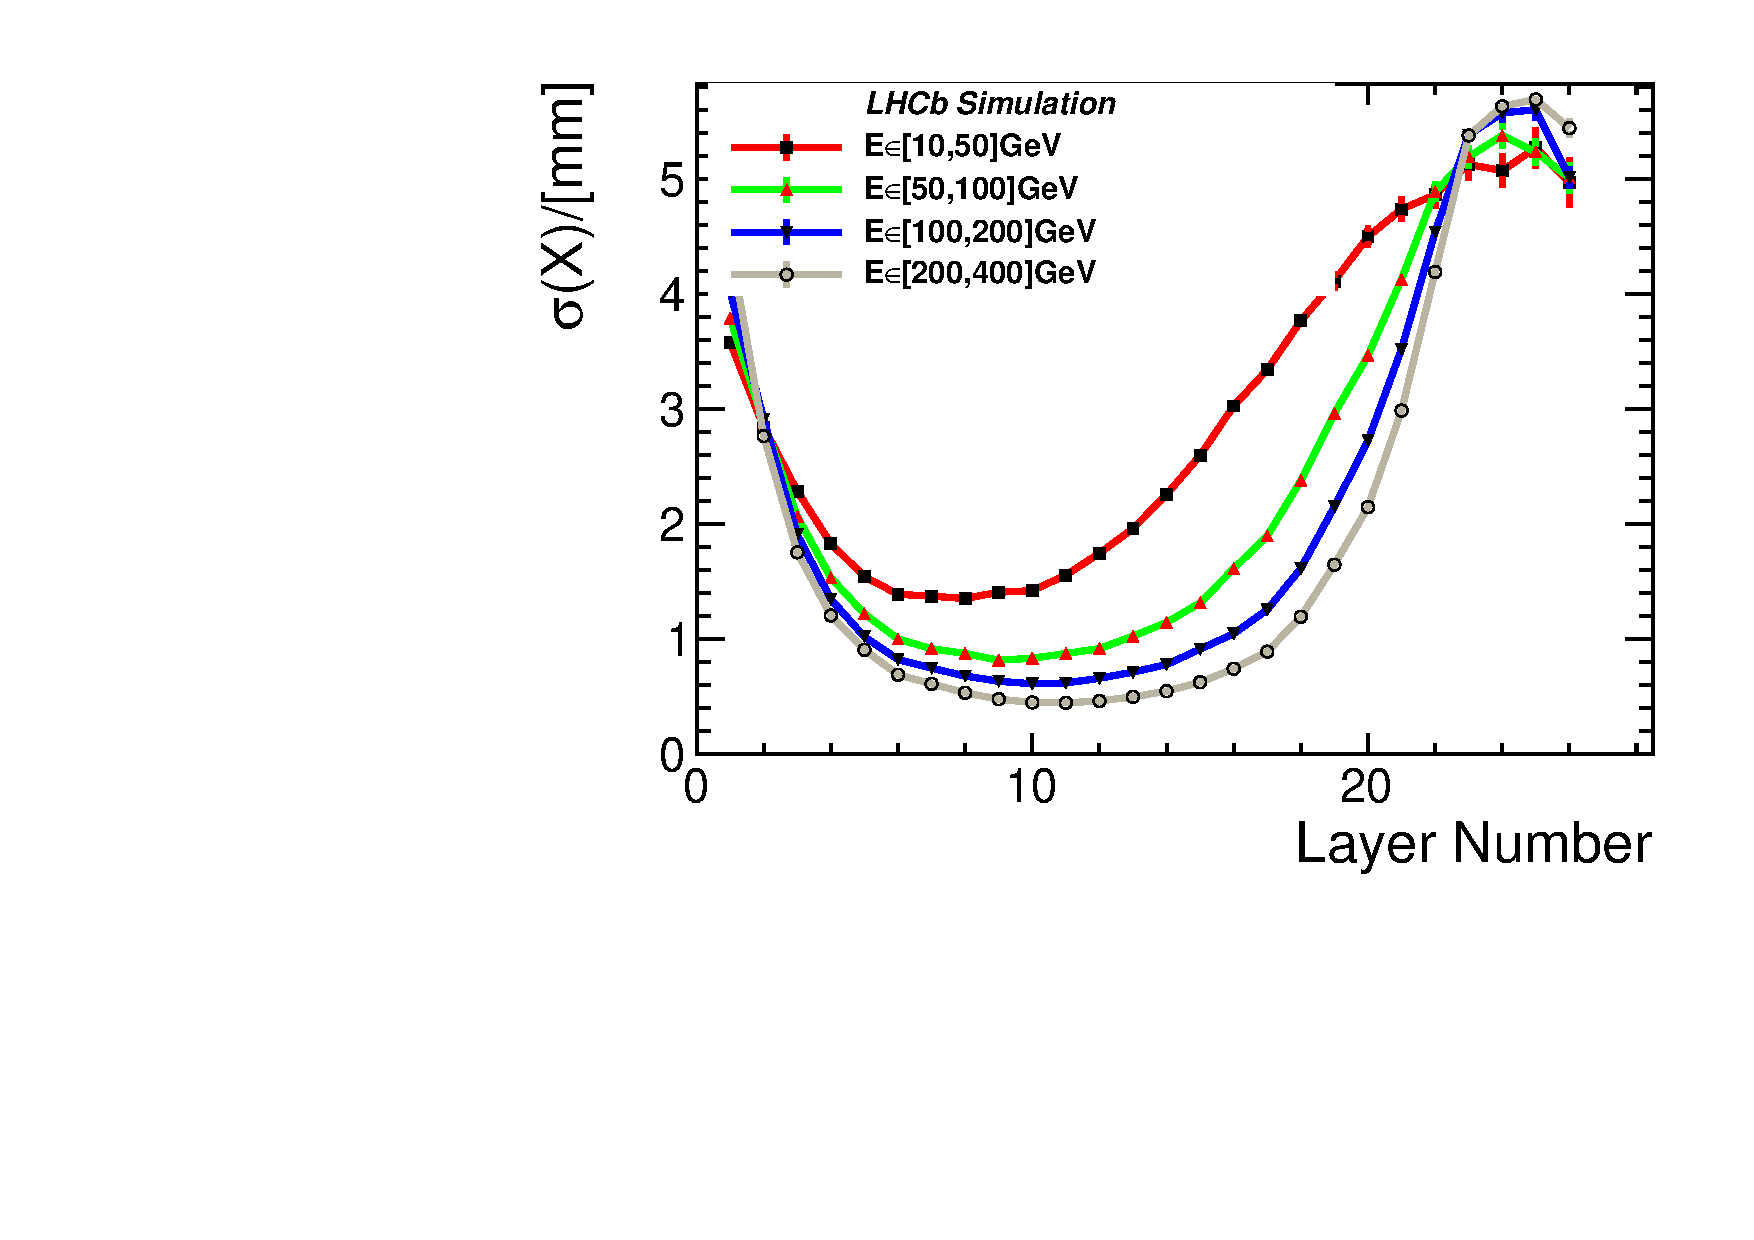
\includegraphics[width=0.53\textwidth]{Figures/06_ECAL/position_res_cali/pos_res.pdf}
\caption{
   The relative position to the cell between true layer cluster and true layer cluster of the 15th layer (left).
	The position resolution (right).} 
\label{fig:position_rela}
\end{figure}

We also take a look at the position resolution with the different particle energy in each layer.
As shown in the right Figure.~\ref{fig:position_rela},
the 5-17 layer performed better than other layers within a large particle gun energy region.

%\begin{figure}[!tbp]
%\centering
%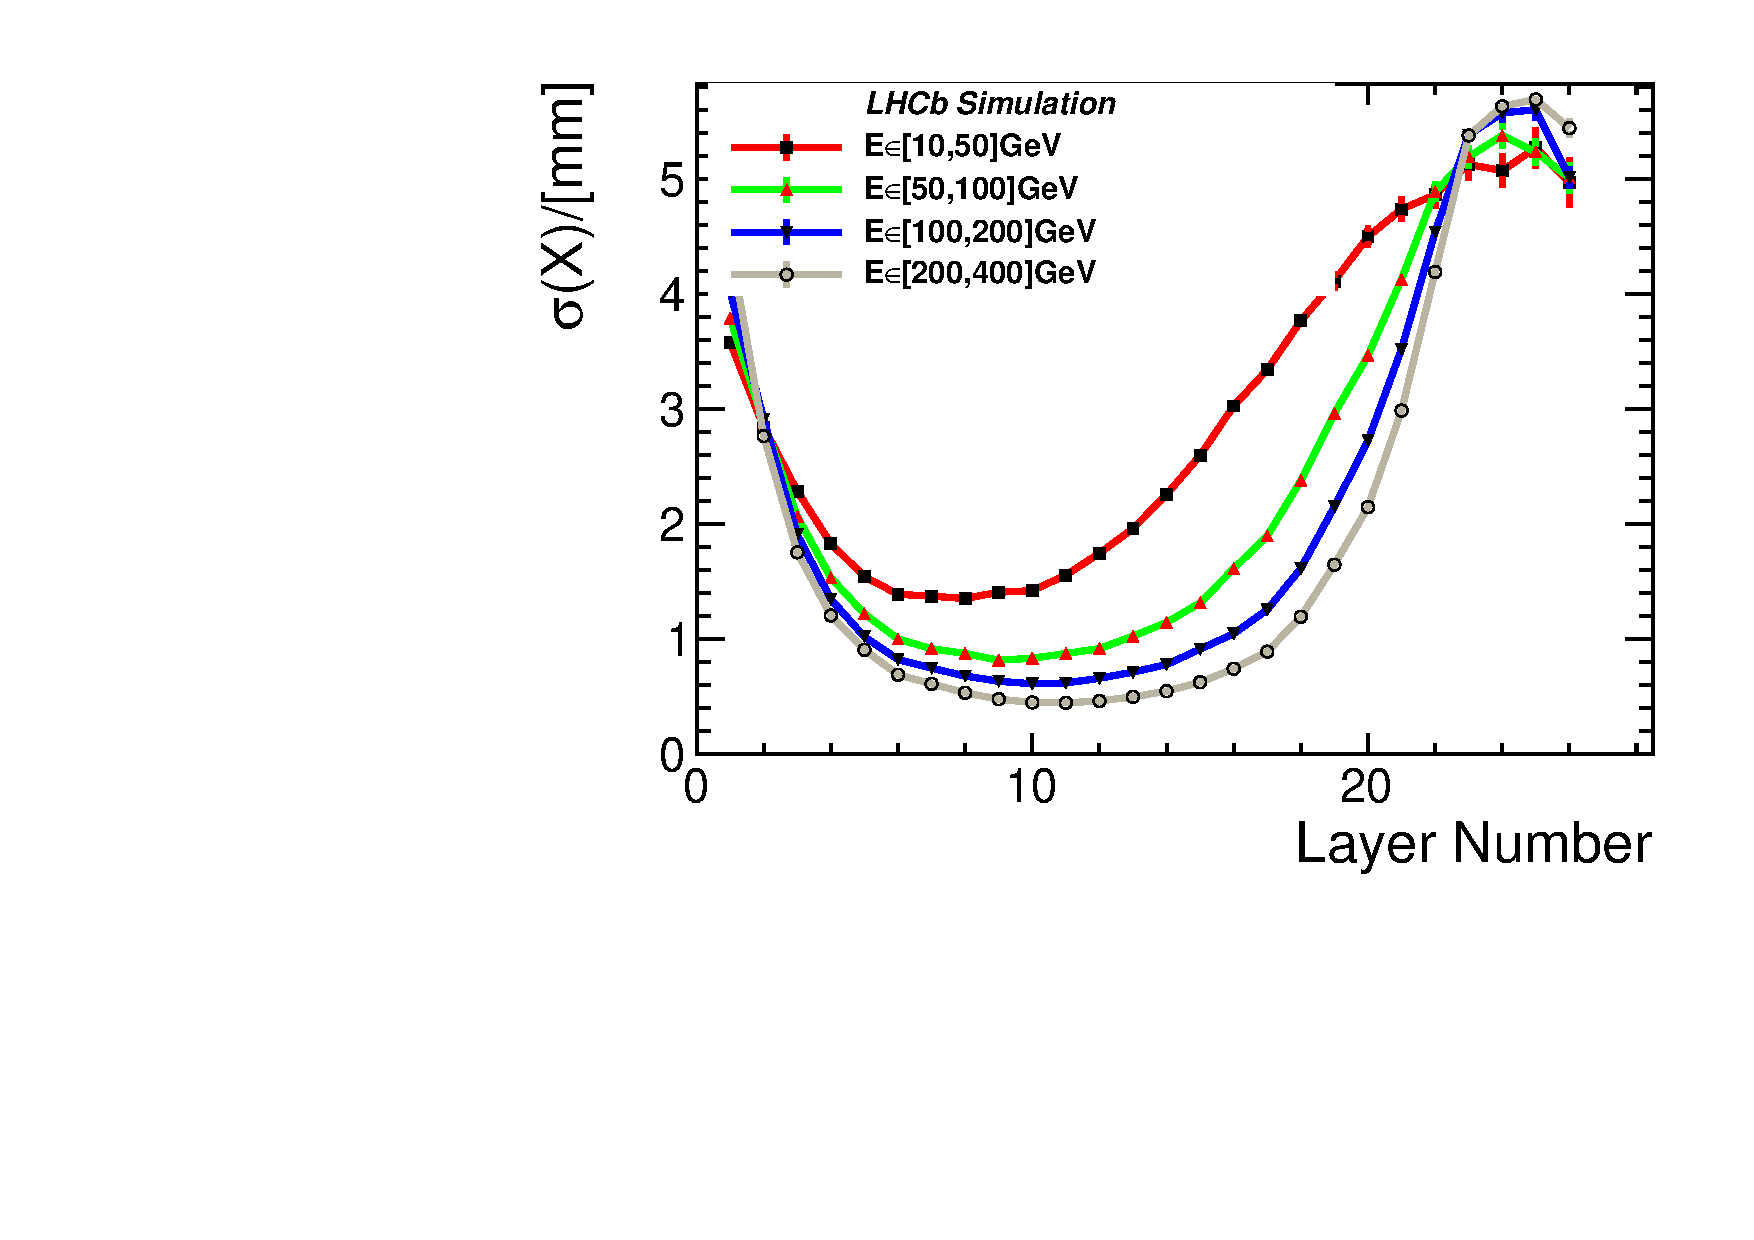
\includegraphics[width=0.6\textwidth]{Figures/06_ECAL/position_res_cali/pos_res.pdf}
%\caption{The position resolution.} 
%\label{fig:position_res}
%\end{figure}



\subsubsection{Timing calibration}

The method to calibrate time information is also studied.
As mentioned in the Section.~\ref{subsubsec:para_time}, 
the parameterized method is used to simulate the silicon sensor time, 
which also rest with the development characters of shower in Si-W \ecal.
Usually, the measured time around the seed cell perform a "time-lag" effect comparing to the value obtained from the seed cell.
As shown in Figure.~\ref{fig:time_cali},
the time difference measured from the seed cell and around cells is related to the distance,
in this case, 
we calibrate the cell time using a linear function:
\begin{equation}
\Delta(T_{cell}) = a \times d + b
\end{equation}
where the $\Delta(T_{cell})$ is the time difference to the seed cell, 
$d$ is the distance,
and $a,b$ are the calibration parameters.
We study the time calibration for each layer seperately.

\begin{figure}[!thbp]
 \centering
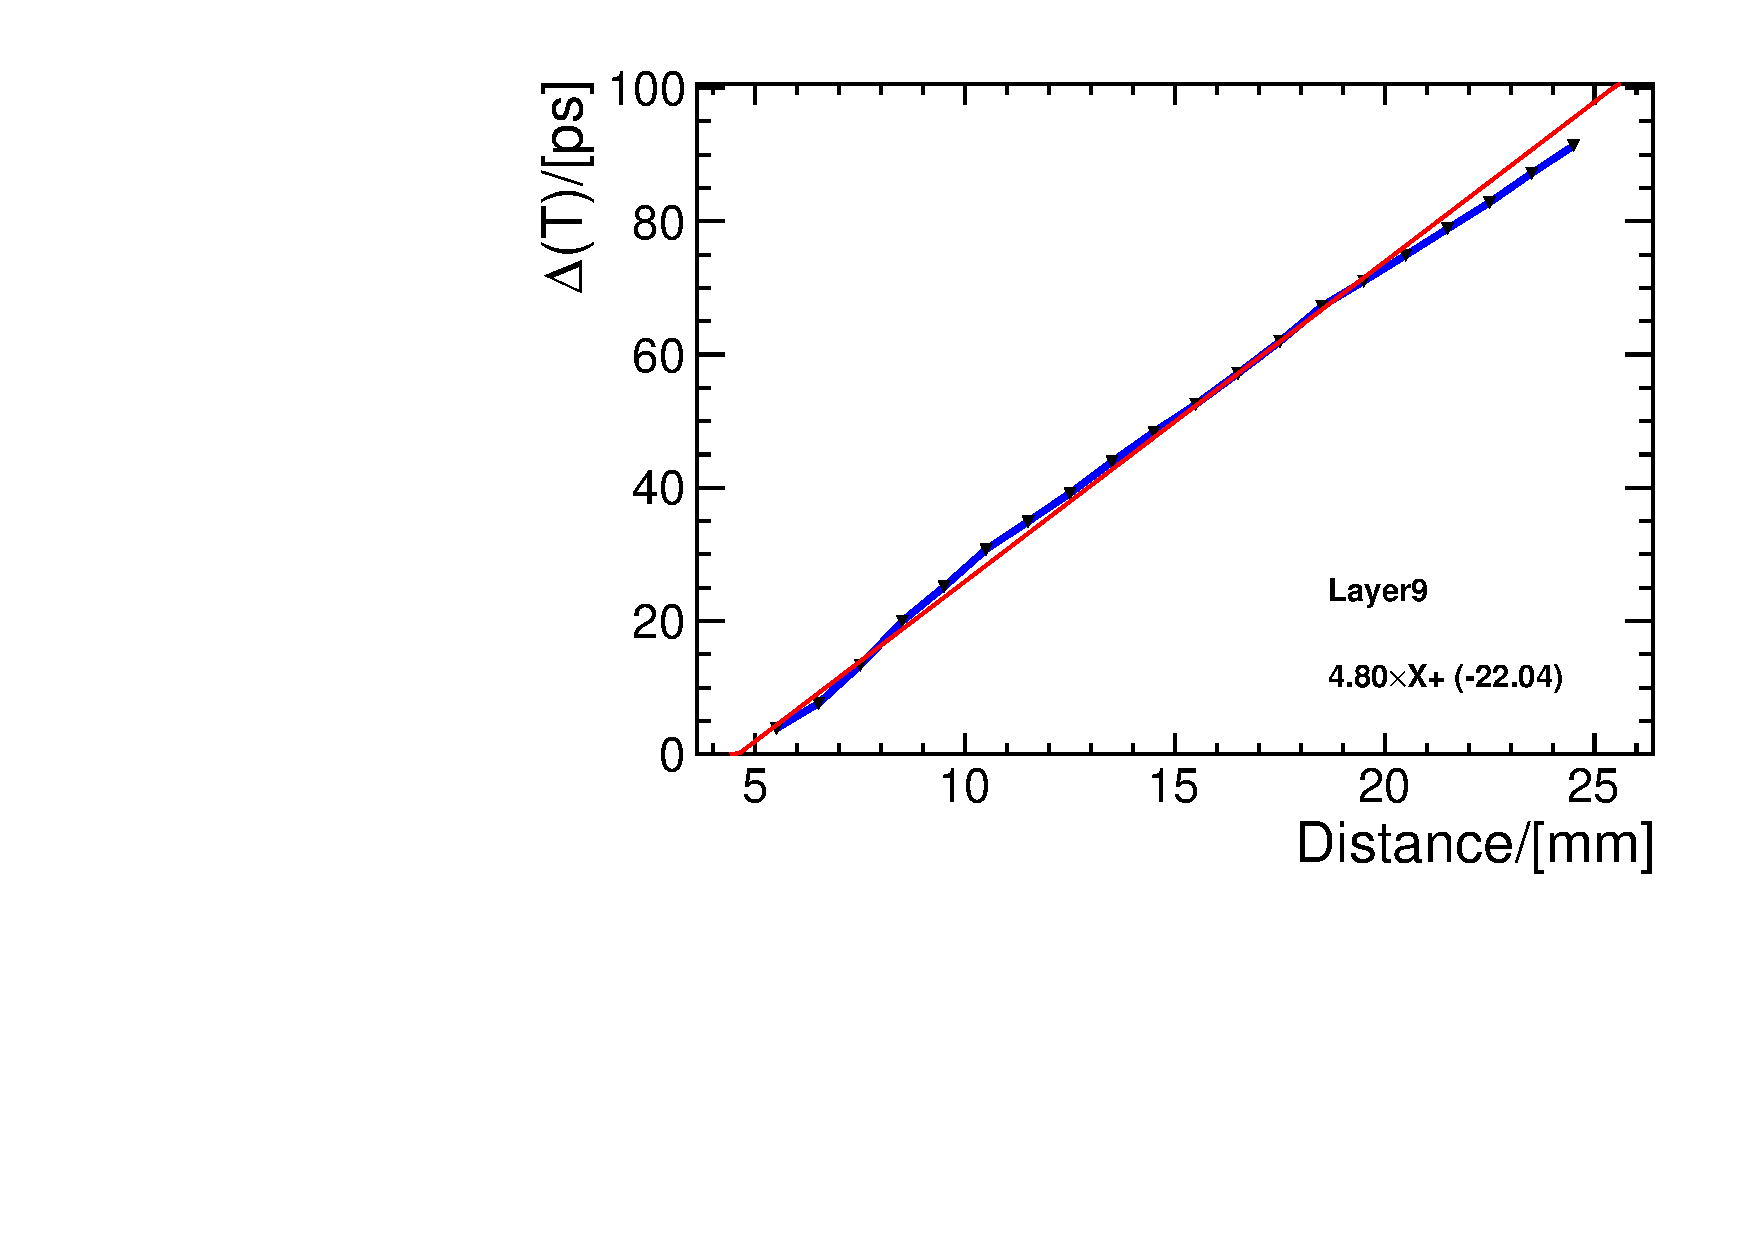
\includegraphics[width=0.5\textwidth]{Figures/06_ECAL/time_cali_res/E_fraction_layers_9.pdf}
\caption{The time difference between the seed cell time with the measured value around cells in 9th layer} 
\label{fig:time_cali}
\end{figure}

The time resolutions of every layer are shown in Figure.~\ref{fig:time_layer_res},
which are different with each other as the shower deposited energy distribution in the z-direction.
According to the energy resolution results in every layer mentioned above, 
we find that the layer with larger deposited energy leads to better energy and time resolution.


\begin{figure}[!thbp]
\centering
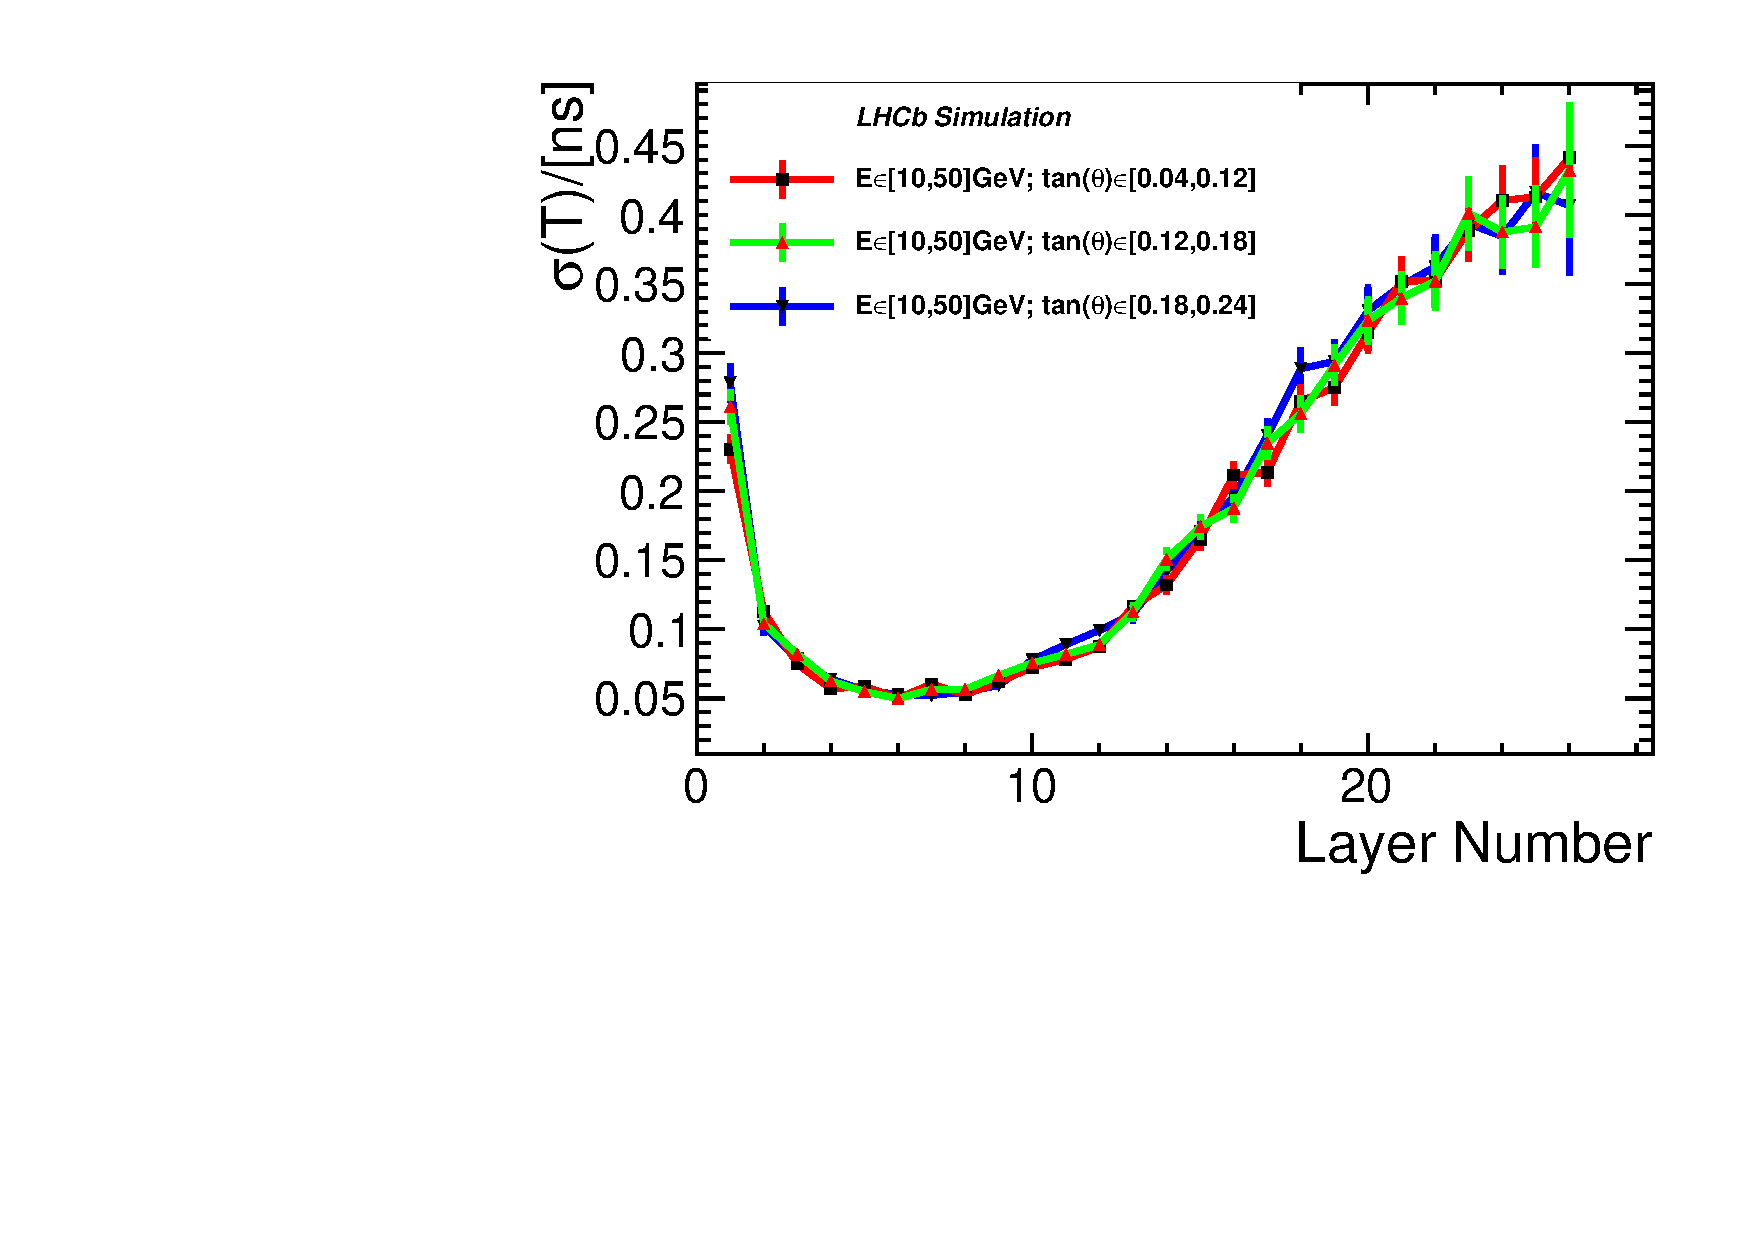
\includegraphics[width=0.45\textwidth]{Figures/06_ECAL/time_cali_res/Time_res_50.pdf}
\put(-130,60) {\textrm{\small \bf(a)}}
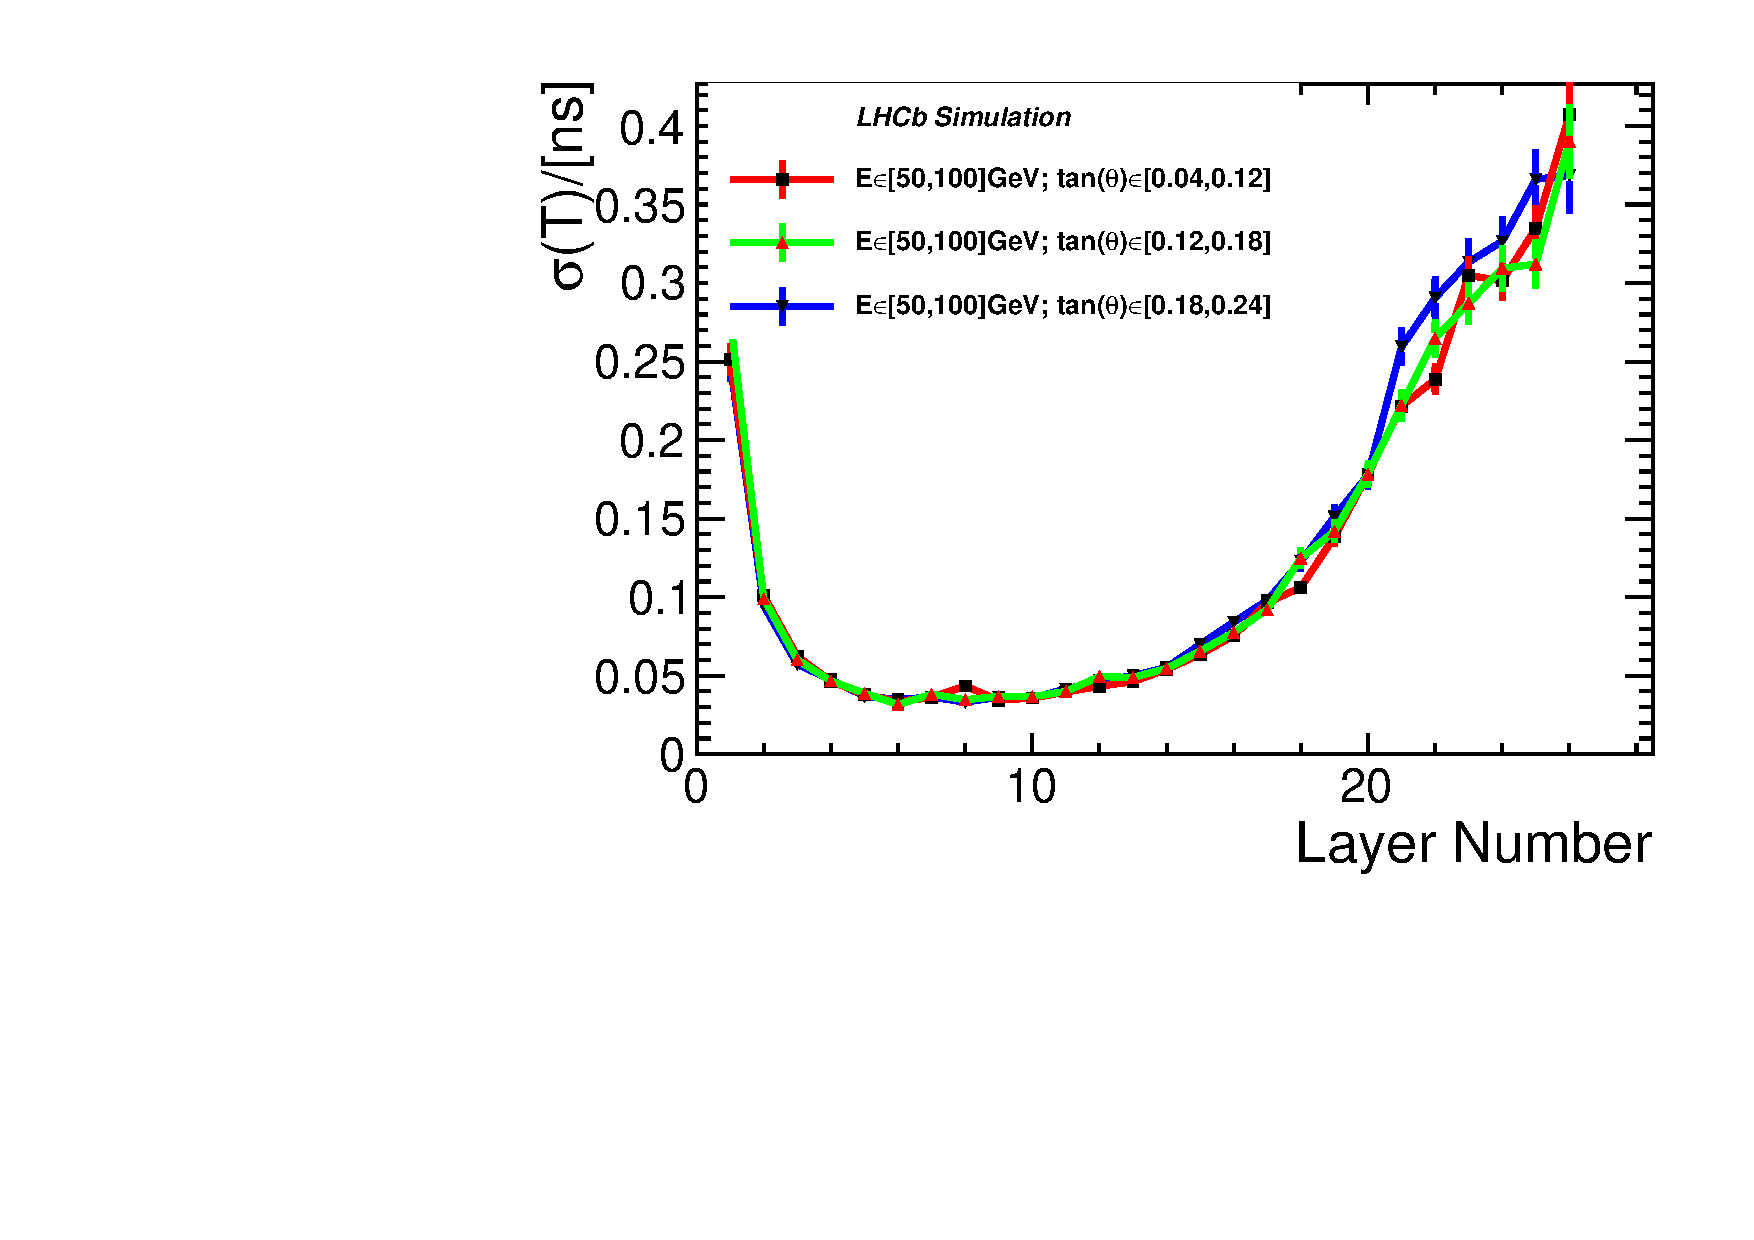
\includegraphics[width=0.45\textwidth]{Figures/06_ECAL/time_cali_res/Time_res_100.pdf}
\put(-130,60) {\textrm{\small \bf(b)}}\\
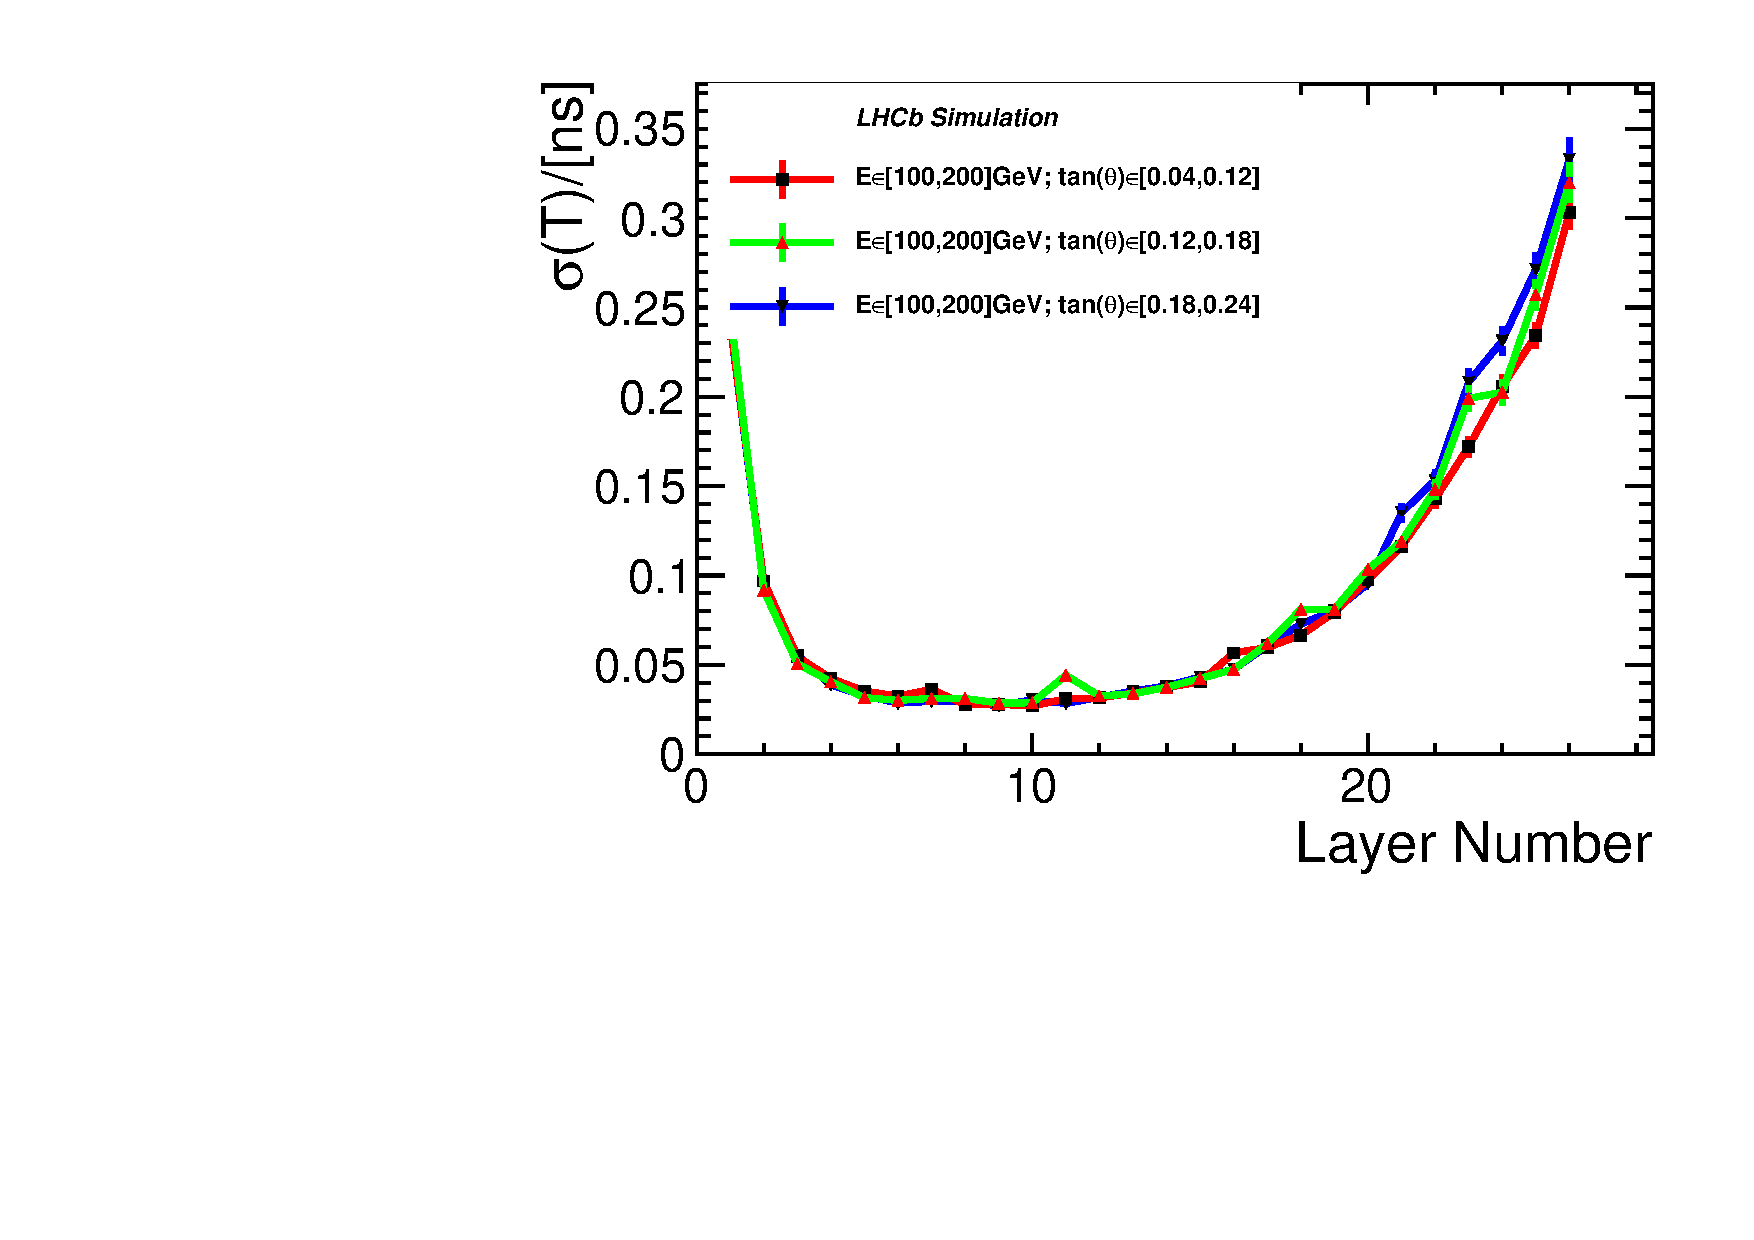
\includegraphics[width=0.45\textwidth]{Figures/06_ECAL/time_cali_res/Time_res_200.pdf}
\put(-130,60) {\textrm{\small \bf(c)}}
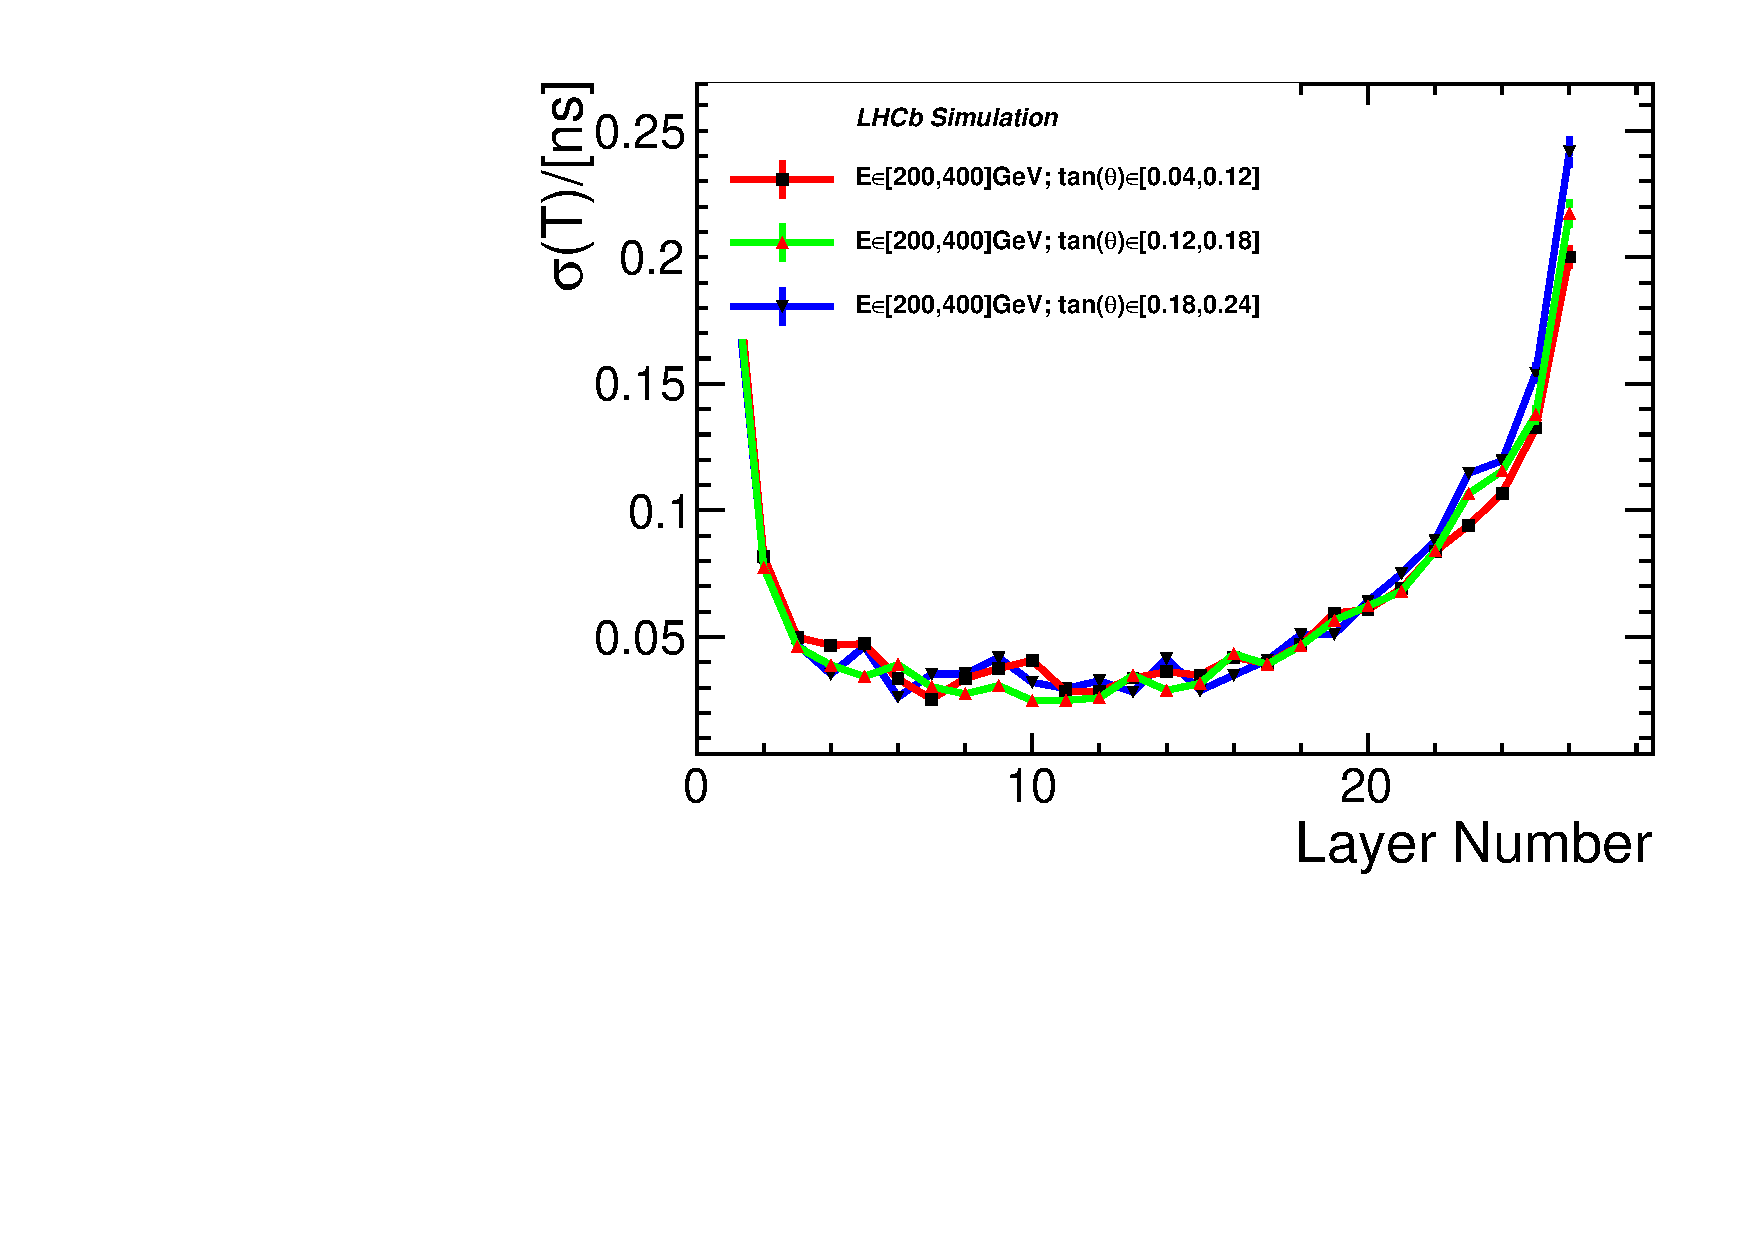
\includegraphics[width=0.45\textwidth]{Figures/06_ECAL/time_cali_res/Time_res_400.pdf}
\put(-130,60) {\textrm{\small \bf(d)}}
\caption{The time resolution of each layer with different $\gamma$ energy and incident angle.} 
\label{fig:time_layer_res}
\end{figure}

Figure.~\ref{fig:time_layer_res_com} shows the time resolution in layer 4-14 before and after the cell time calibration,
the time distribution peak becomes narrow, especially for the rear layers.

\begin{figure}[!thbp]
\centering
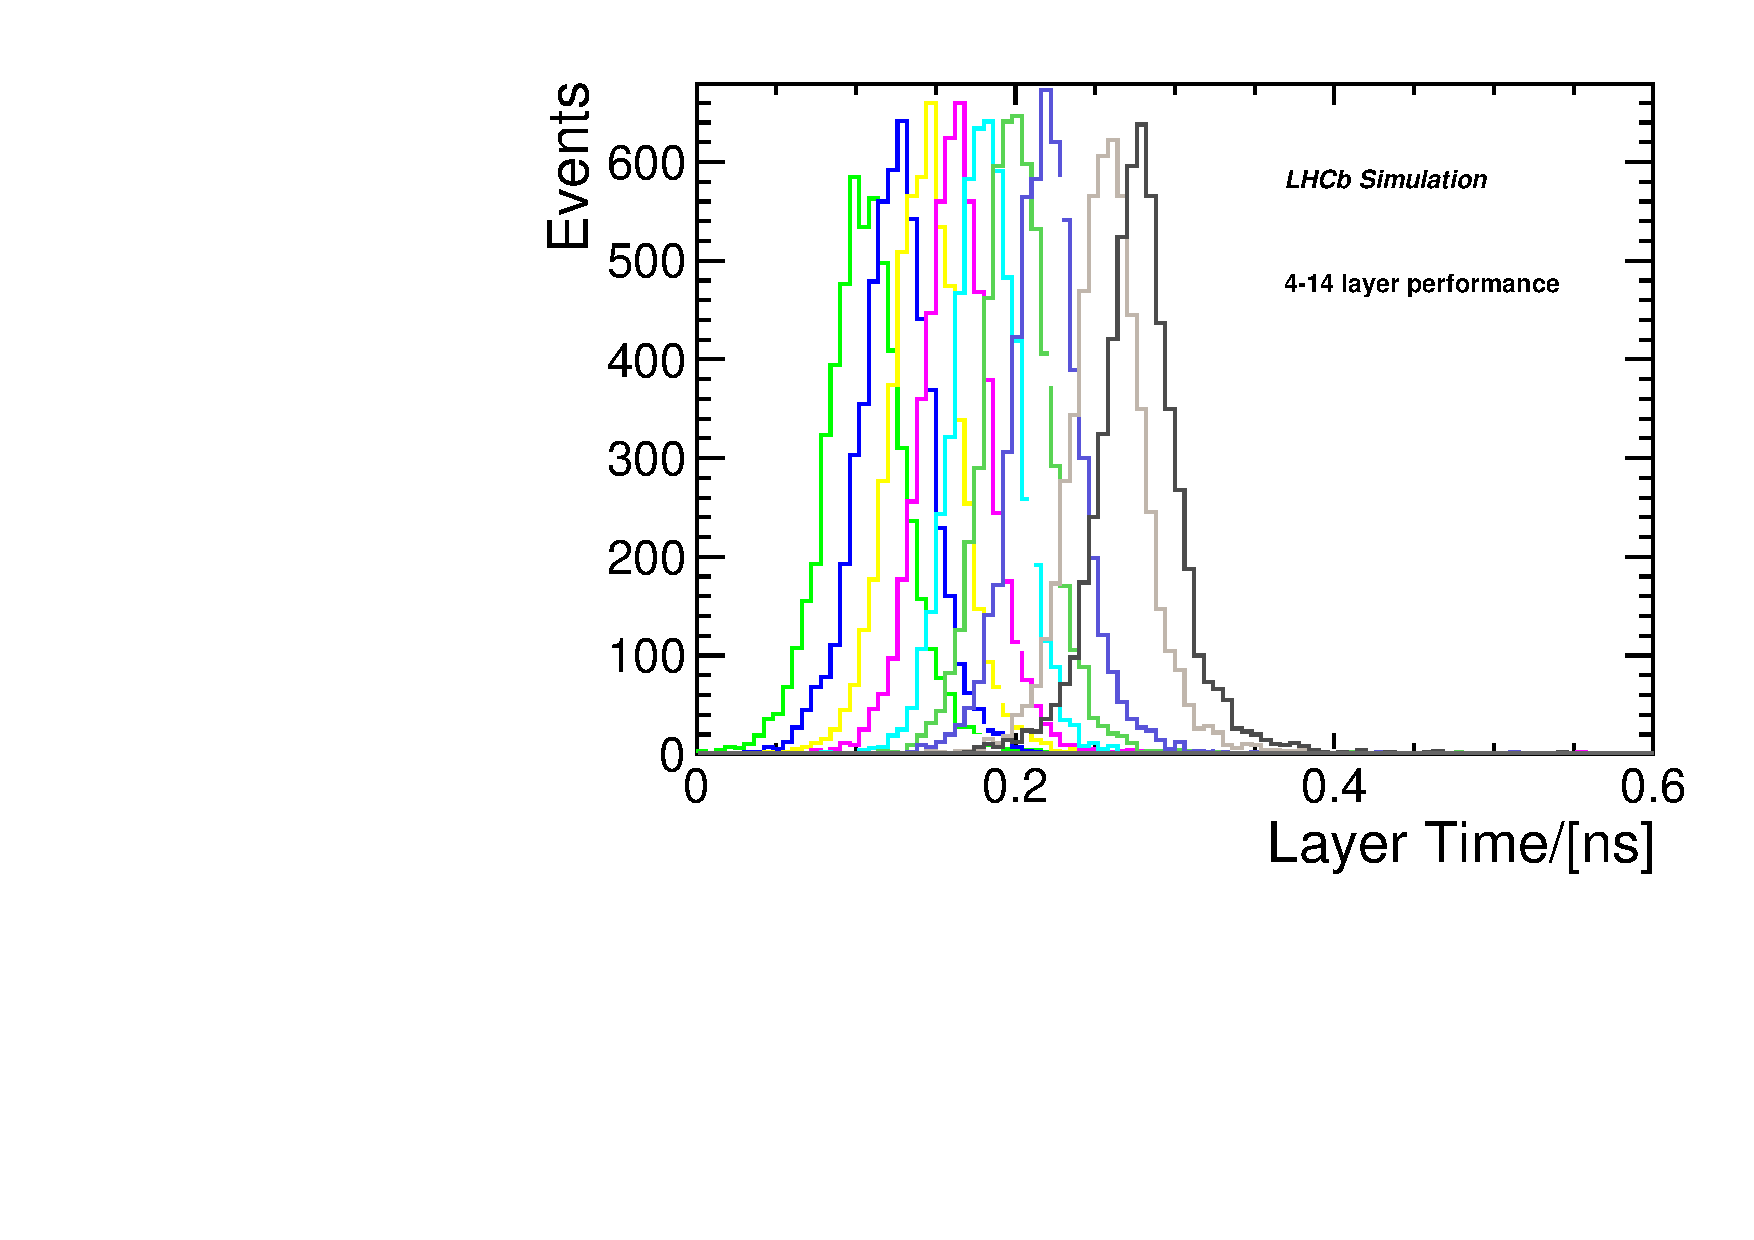
\includegraphics[width=0.45\textwidth]{Figures/06_ECAL/time_cali_res/before_time_cali.pdf}
\put(-60,60) {\textrm{\small \bf(a)}}
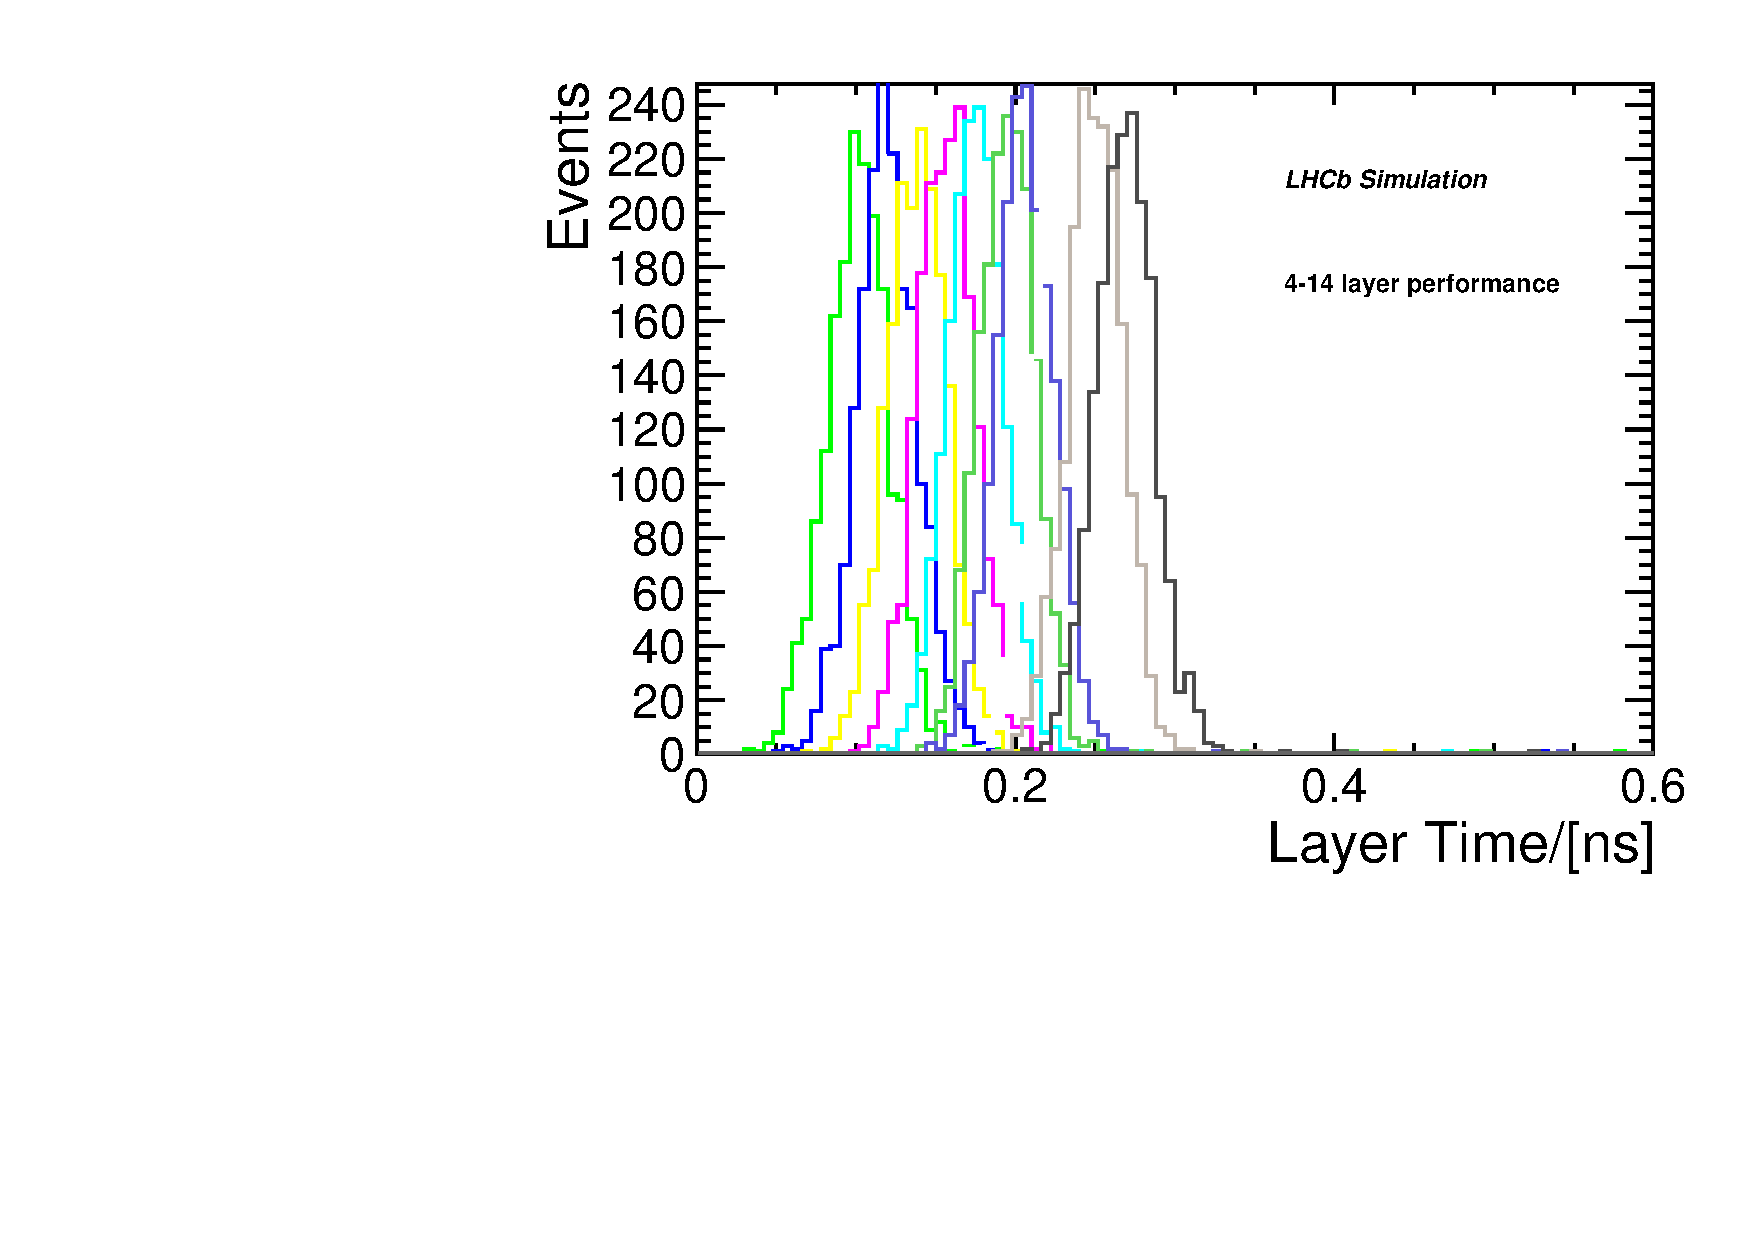
\includegraphics[width=0.45\textwidth]{Figures/06_ECAL/time_cali_res/after_time_cali.pdf}
\put(-60,60) {\textrm{\small \bf(b)}}\\
\caption{The time distribution for each layer before(a) and after(b) calibration.} 
\label{fig:time_layer_res_com}
\end{figure}

The shower time is reconstucted based on the measured time from each layer,
the time recorded in each layer is different as shower developing in the longitudinal direction.
As shown in Figure.~\ref{fig:time_shower_layer},
the slope of this linear function obtained from fitting is around equal the value if assume the shower development speed is exactly equal to light speed,
from this study,
which is around $2\%$ smaller than the light speed.
Besides, 
we use this parameter to calibrate the measured layer time when reconstruct the shower time.

\begin{figure}[!thbp]
\centering
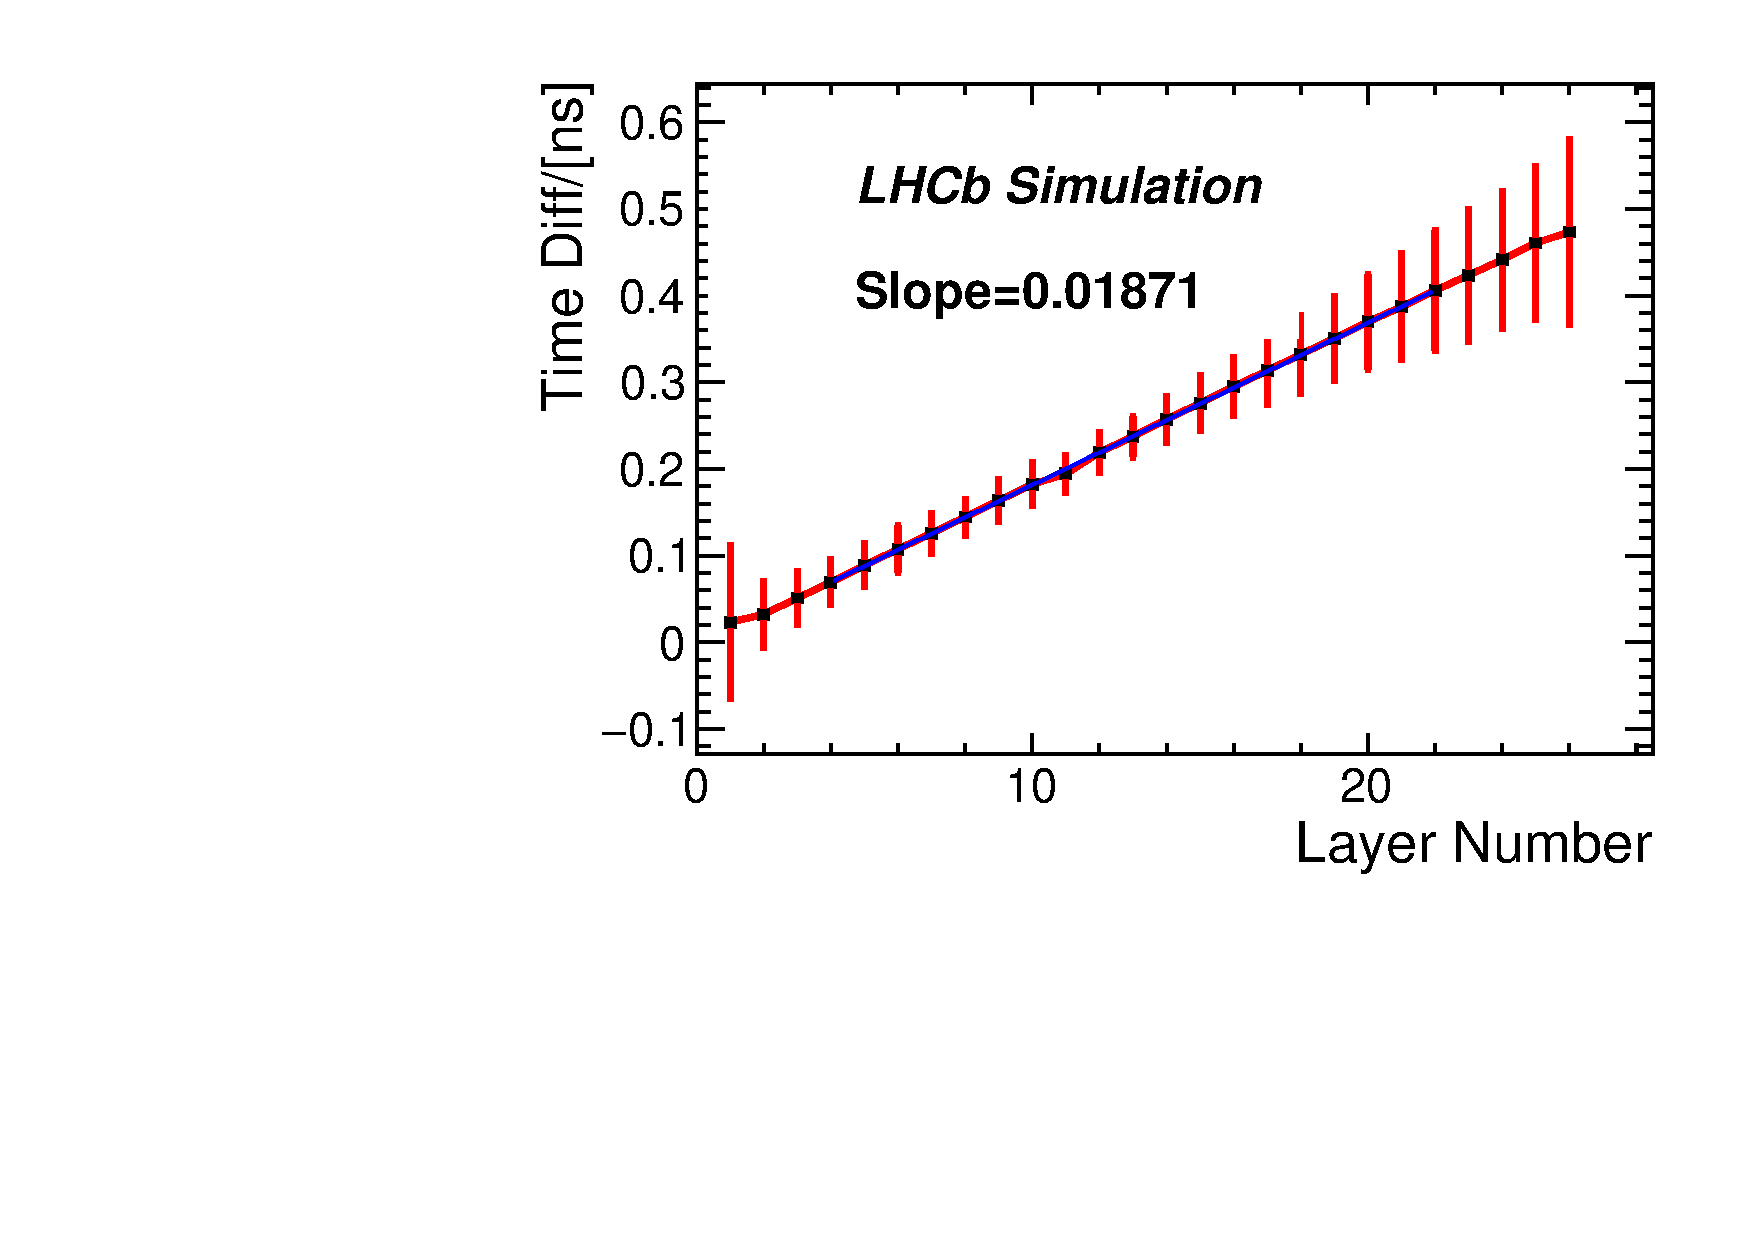
\includegraphics[width=0.6\textwidth]{Figures/06_ECAL/time_cali_res/rela_layer_time_cali.pdf}
\caption{The time difference measured in each layer.} 
\label{fig:time_shower_layer}
\end{figure}

\begin{figure}[!thbp]
\centering
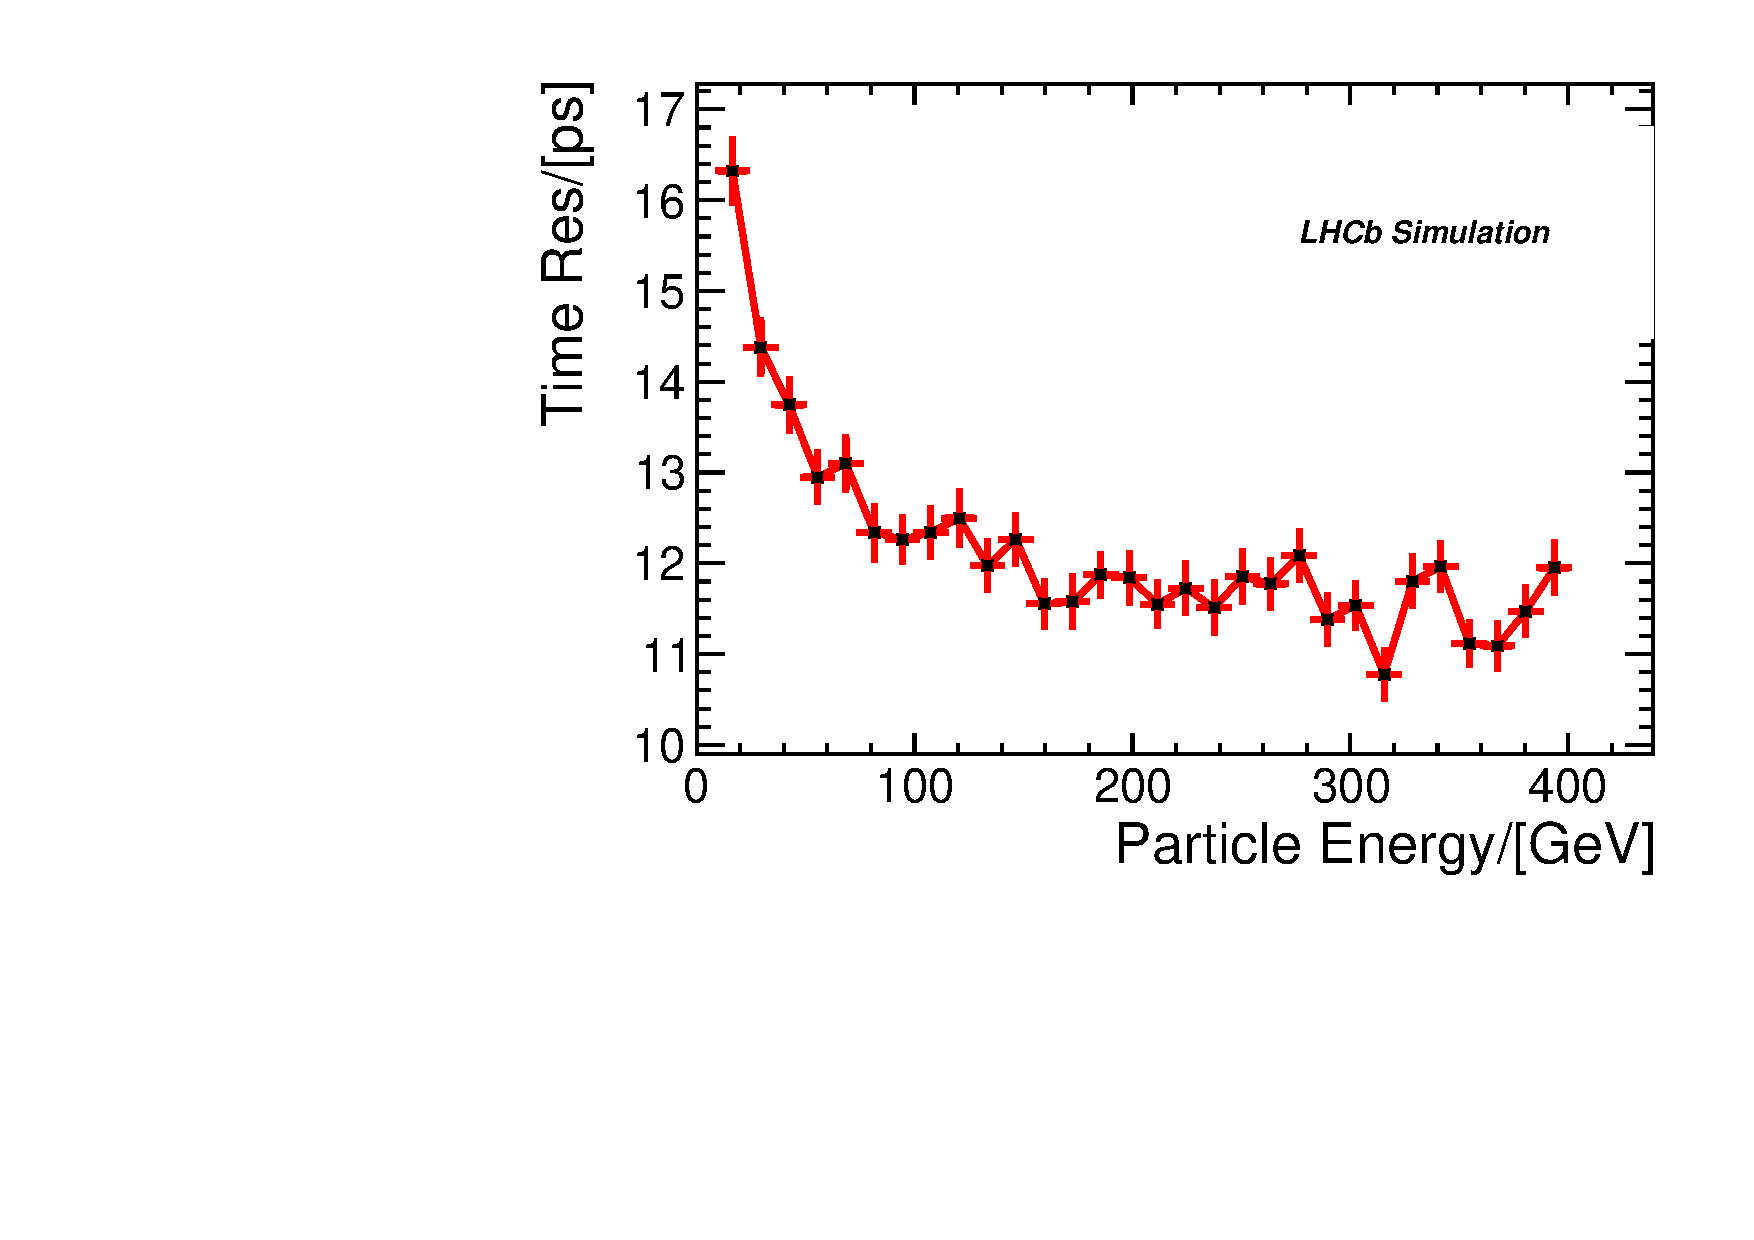
\includegraphics[width=0.45\textwidth]{Figures/06_ECAL/time_cali_res/shower_time_res_6.pdf}
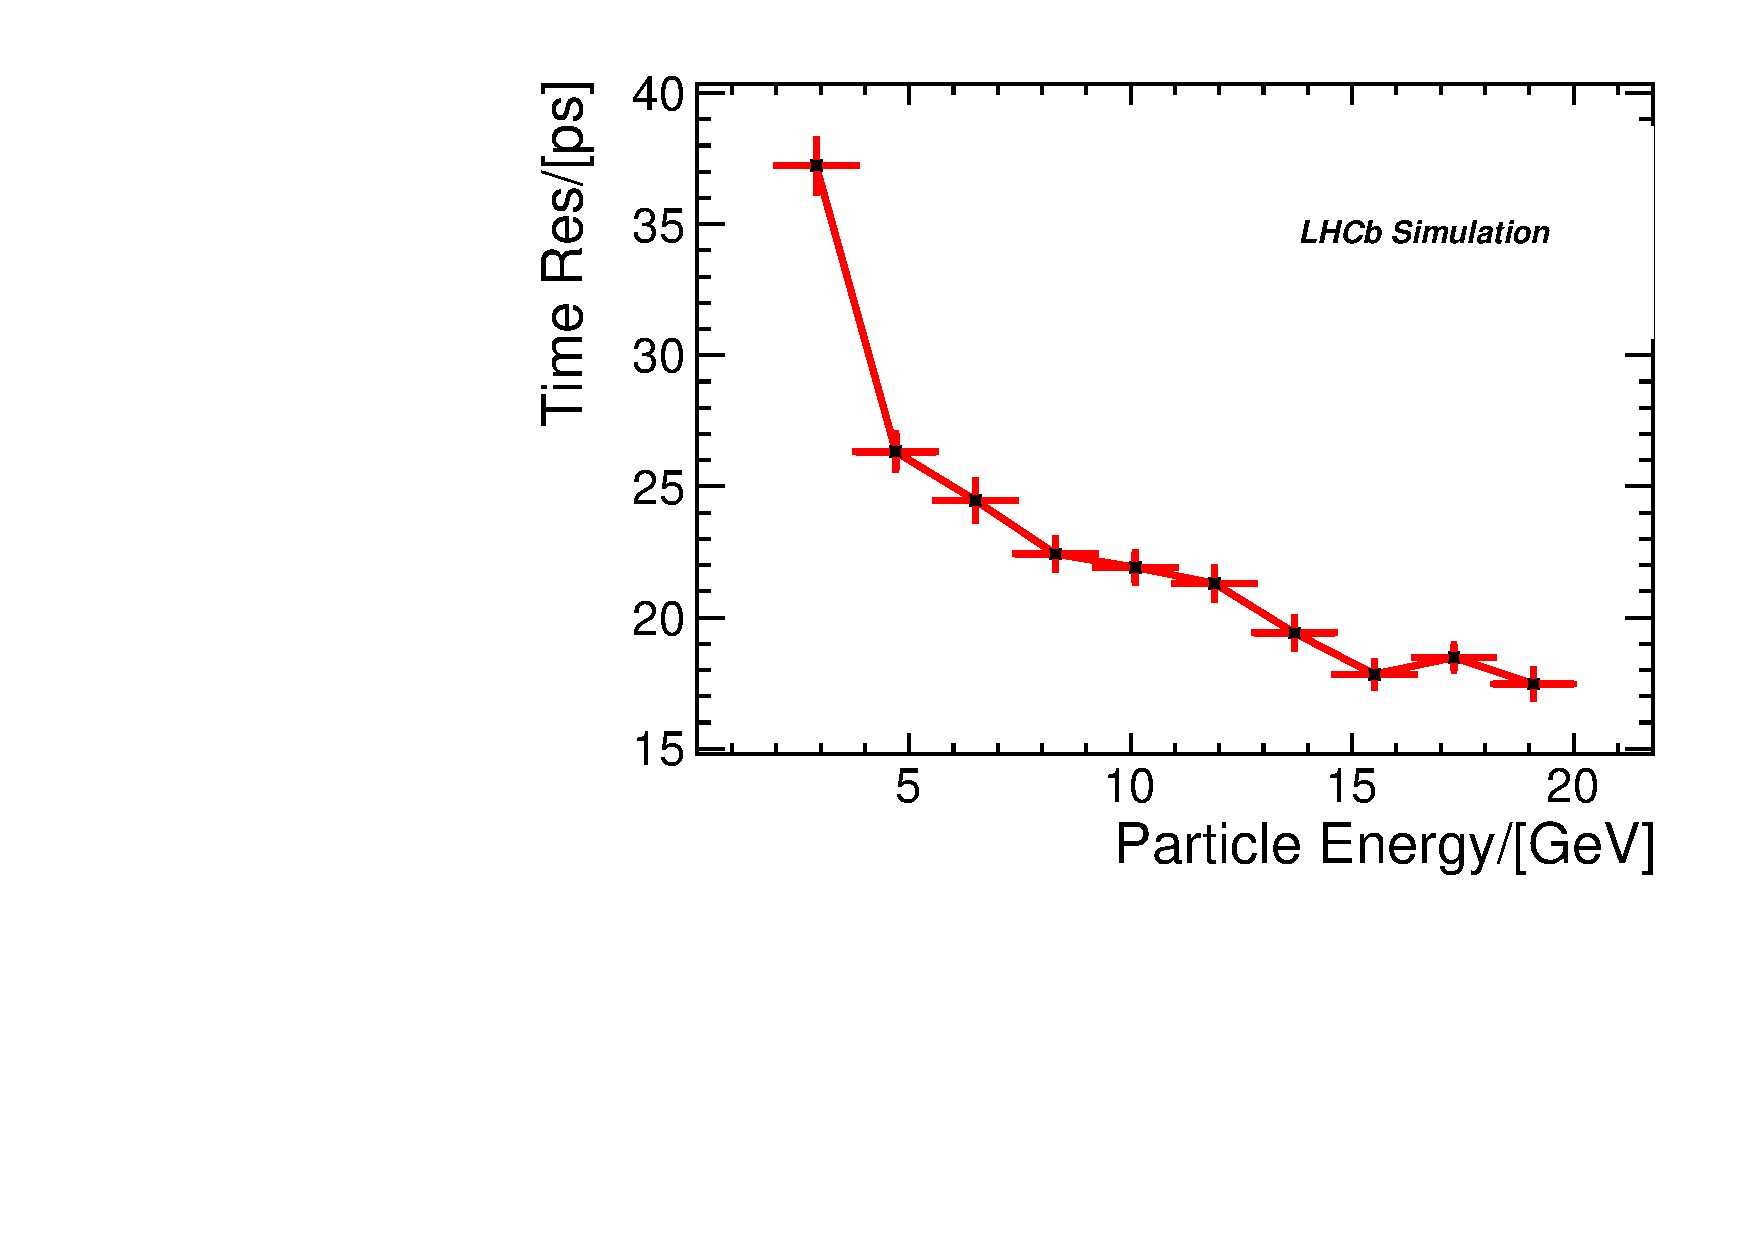
\includegraphics[width=0.45\textwidth]{Figures/06_ECAL/time_cali_res/shower_time_res_6_low_energy.pdf}
\caption{The shower time resolution with three layers to measure shower time, 
the right plot shows the low energy result.} 
\label{fig:time_shower_res}
\end{figure}

After time calibration, 
the shower time resolution is shown in Figure.~\ref{fig:time_shower_res},
which is related to the particle energy,
and the shower time resolution is constructed from 4th, 5th and 6th layers.
If only three layers have the ability to record the time information, 
the shower time resolution will reach to $15\ps$.
This number can meet the requirement obtained from parameterized simualtion. 

%\clearpage
%If the distance between 2$\gamma$ decayed from the $\piz$ in the \ecal plane is large enough,
%the \piz can be reconstructed as resolved one,
%otherwise, 
%it will be reconstructed as merged particle,
%which means the showers from the 2$\gamma$ are overlapping together.
%The reconstruction performance of \piz will reflect the separation ability of this \ecal.
%%The relation between \piz energy and the two $\gamma$ decayed from it is studied first.
%
%%The mass resolution of \piz reflect the energy resolution and position resolution of this kind of \ecal at the same time.
%The distance of two $\gamma$ onto the \ecal plane is related to the \piz energy, as shown in the Fig.~\ref{fig:pi0_distance_E}.
%From the left plot, 
%we find almost all \piz with energy smaller than 150\gev can be reconstructed as resolved \piz,
%as the distance between the decaying two $\gamma$ on the \ecal plane is larger than $30\mm$.
%Actually,
%the \piz energy in some decay channels studied at \lhcb is smaller than 100\gev, 
%such as $\Bs\to\jpsi\piz$, 
%some specific physical channels performance with this high granularity \ecal will be discussed later.
%
%\begin{figure}[!bp]
%\centering
%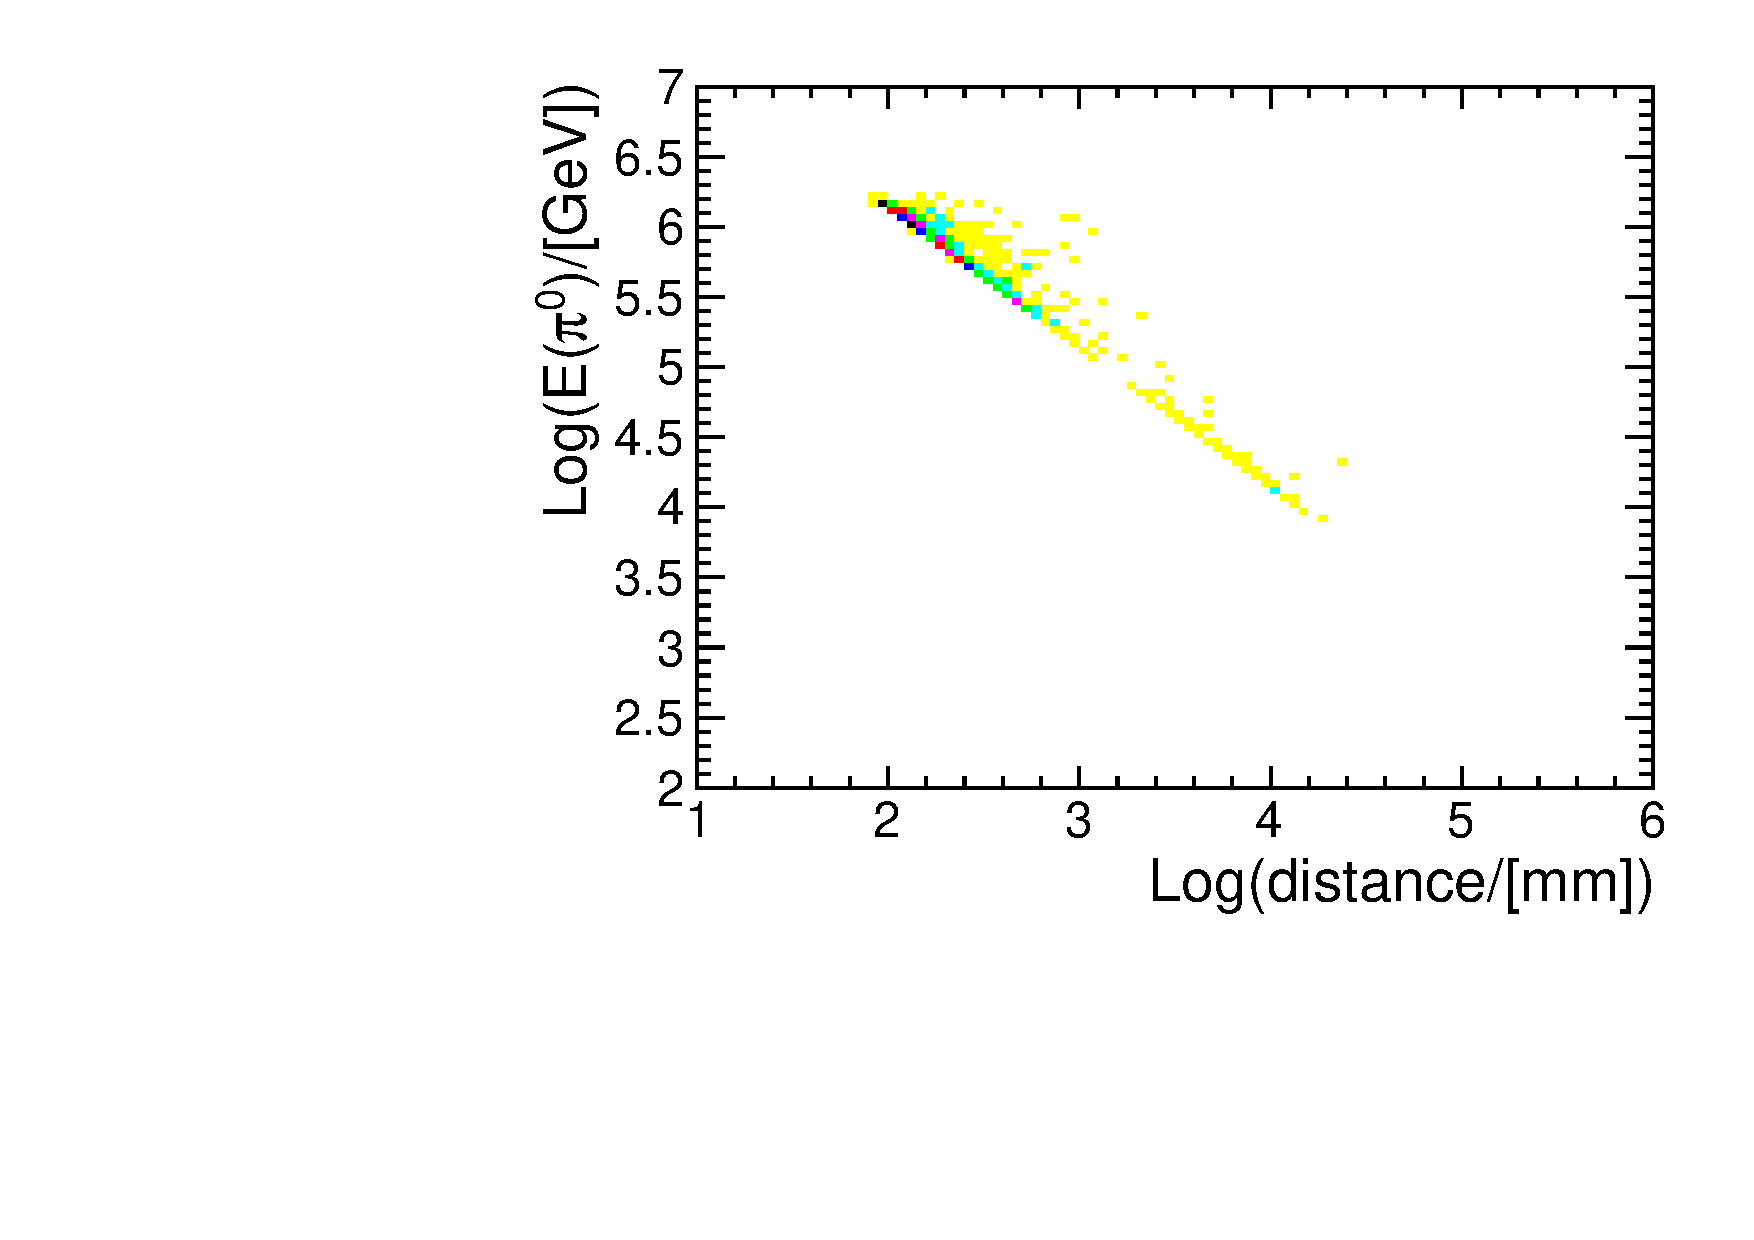
\includegraphics[width=0.45\textwidth]{Figures/06_ECAL/pi0_plots/distance_E.pdf}
%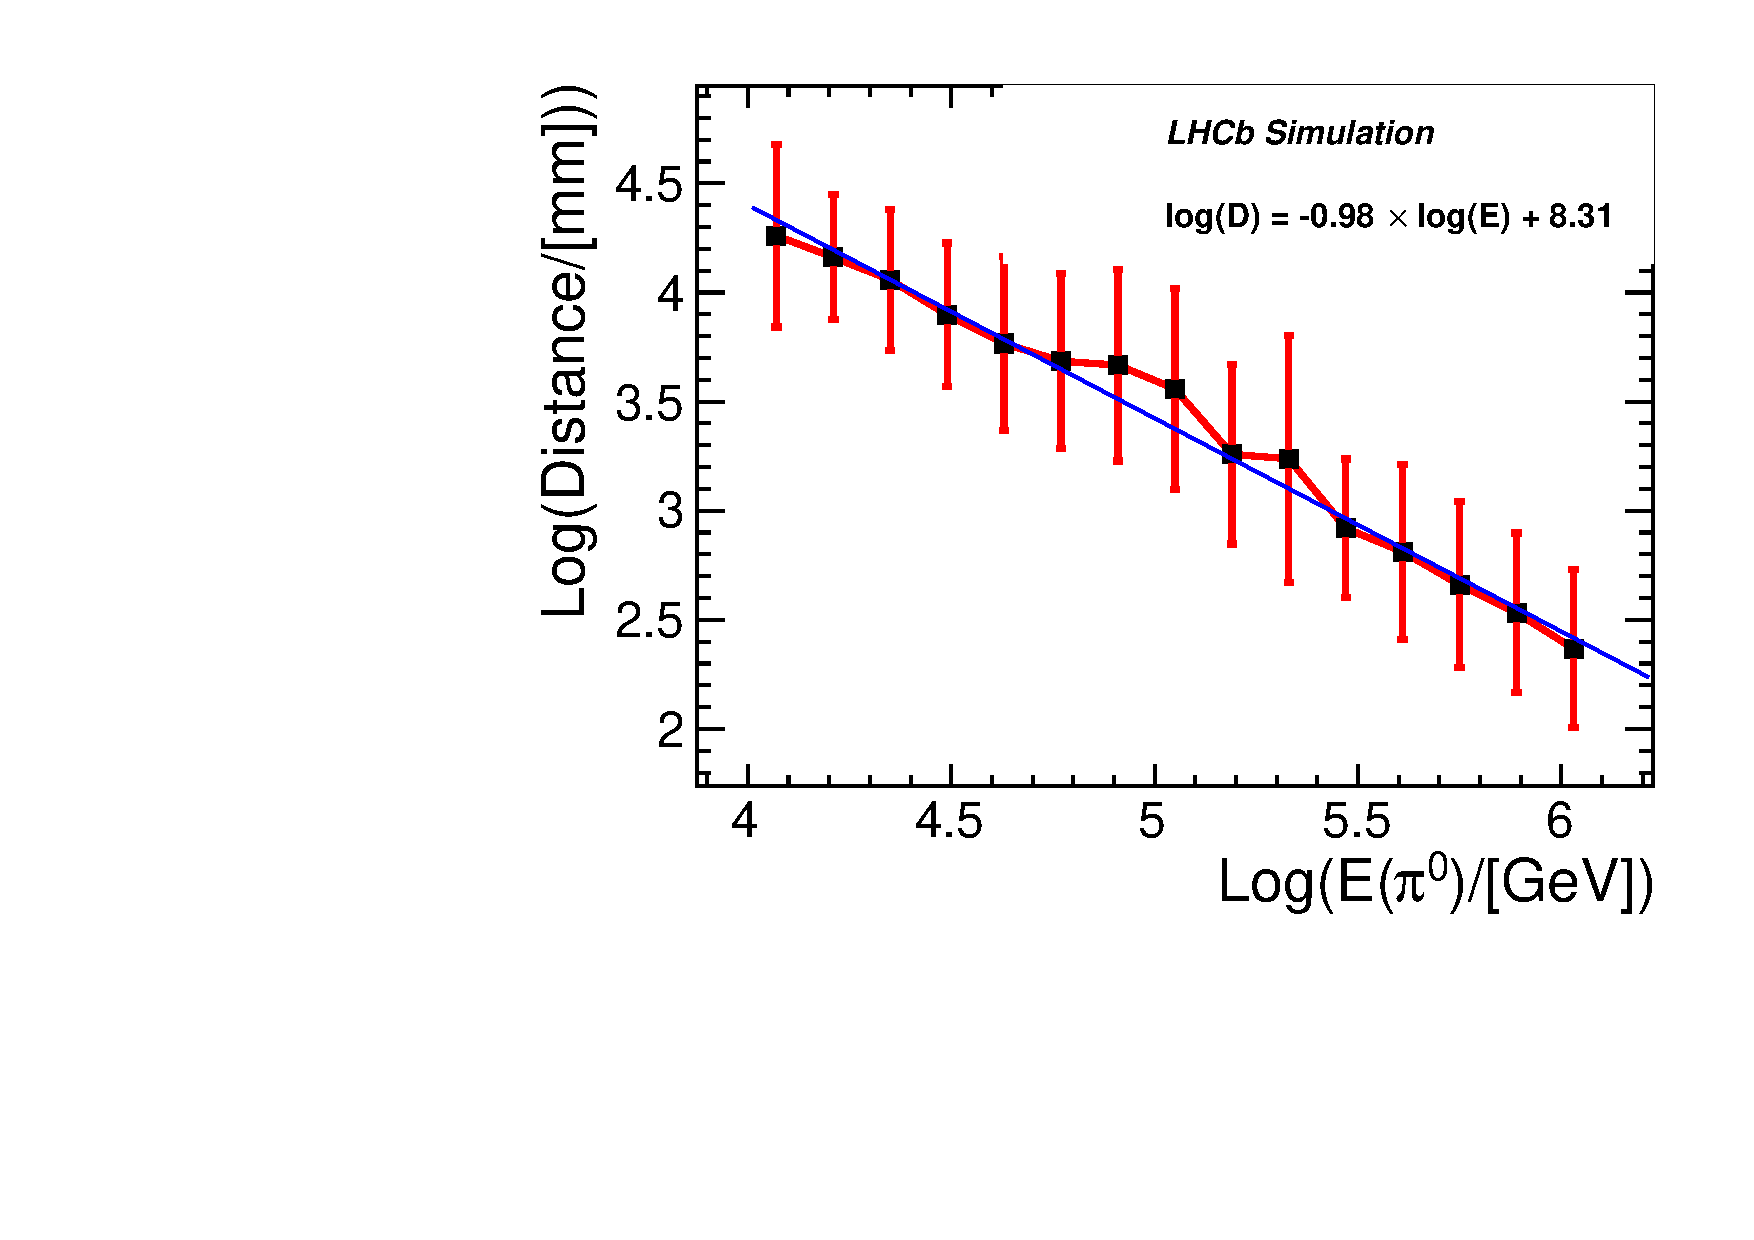
\includegraphics[width=0.45\textwidth]{Figures/06_ECAL/pi0_plots/distance_E_1D.pdf}
%\caption{The relation between the \piz energy and the distance of two $\gamma$ on the \ecal plane.} 
%\label{fig:pi0_distance_E}
%\end{figure}
%
%\subsection{reconstruction of $\piz$ and separation ability}

%\subsubsection{Particle identification}
%The shower in the \ecal can be identified as neutral or charged particle,
%usually, 
%the photons are identified trough some components like shower shape and track-shower matching.
%In this preliminary study, 
%the shower have a large distance to the charged track on the \ecal plane is identified as a neutral particle.
%
%\begin{figure}[!htbp]
%\centering
%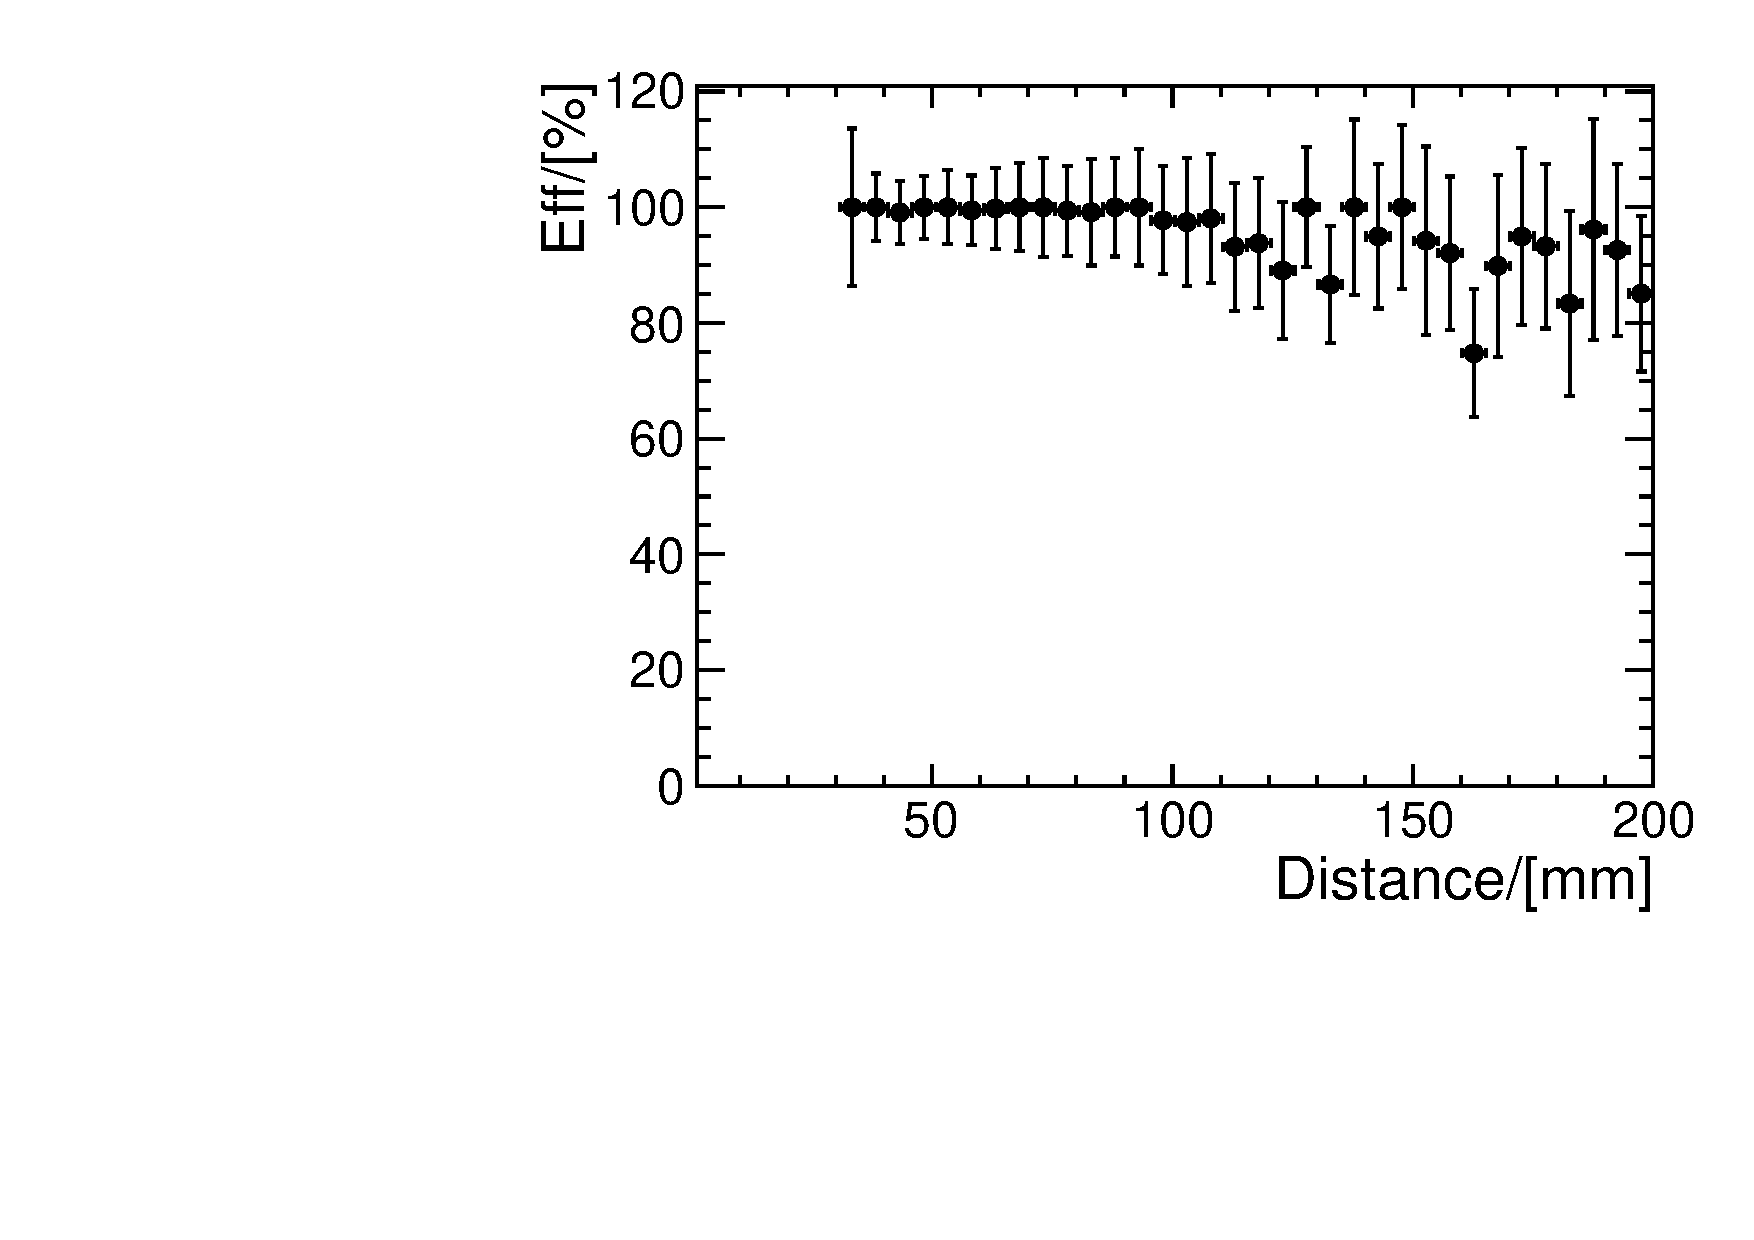
\includegraphics[width=0.45\textwidth]{Figures/06_ECAL/pi0_plots/distance_eff.pdf}
%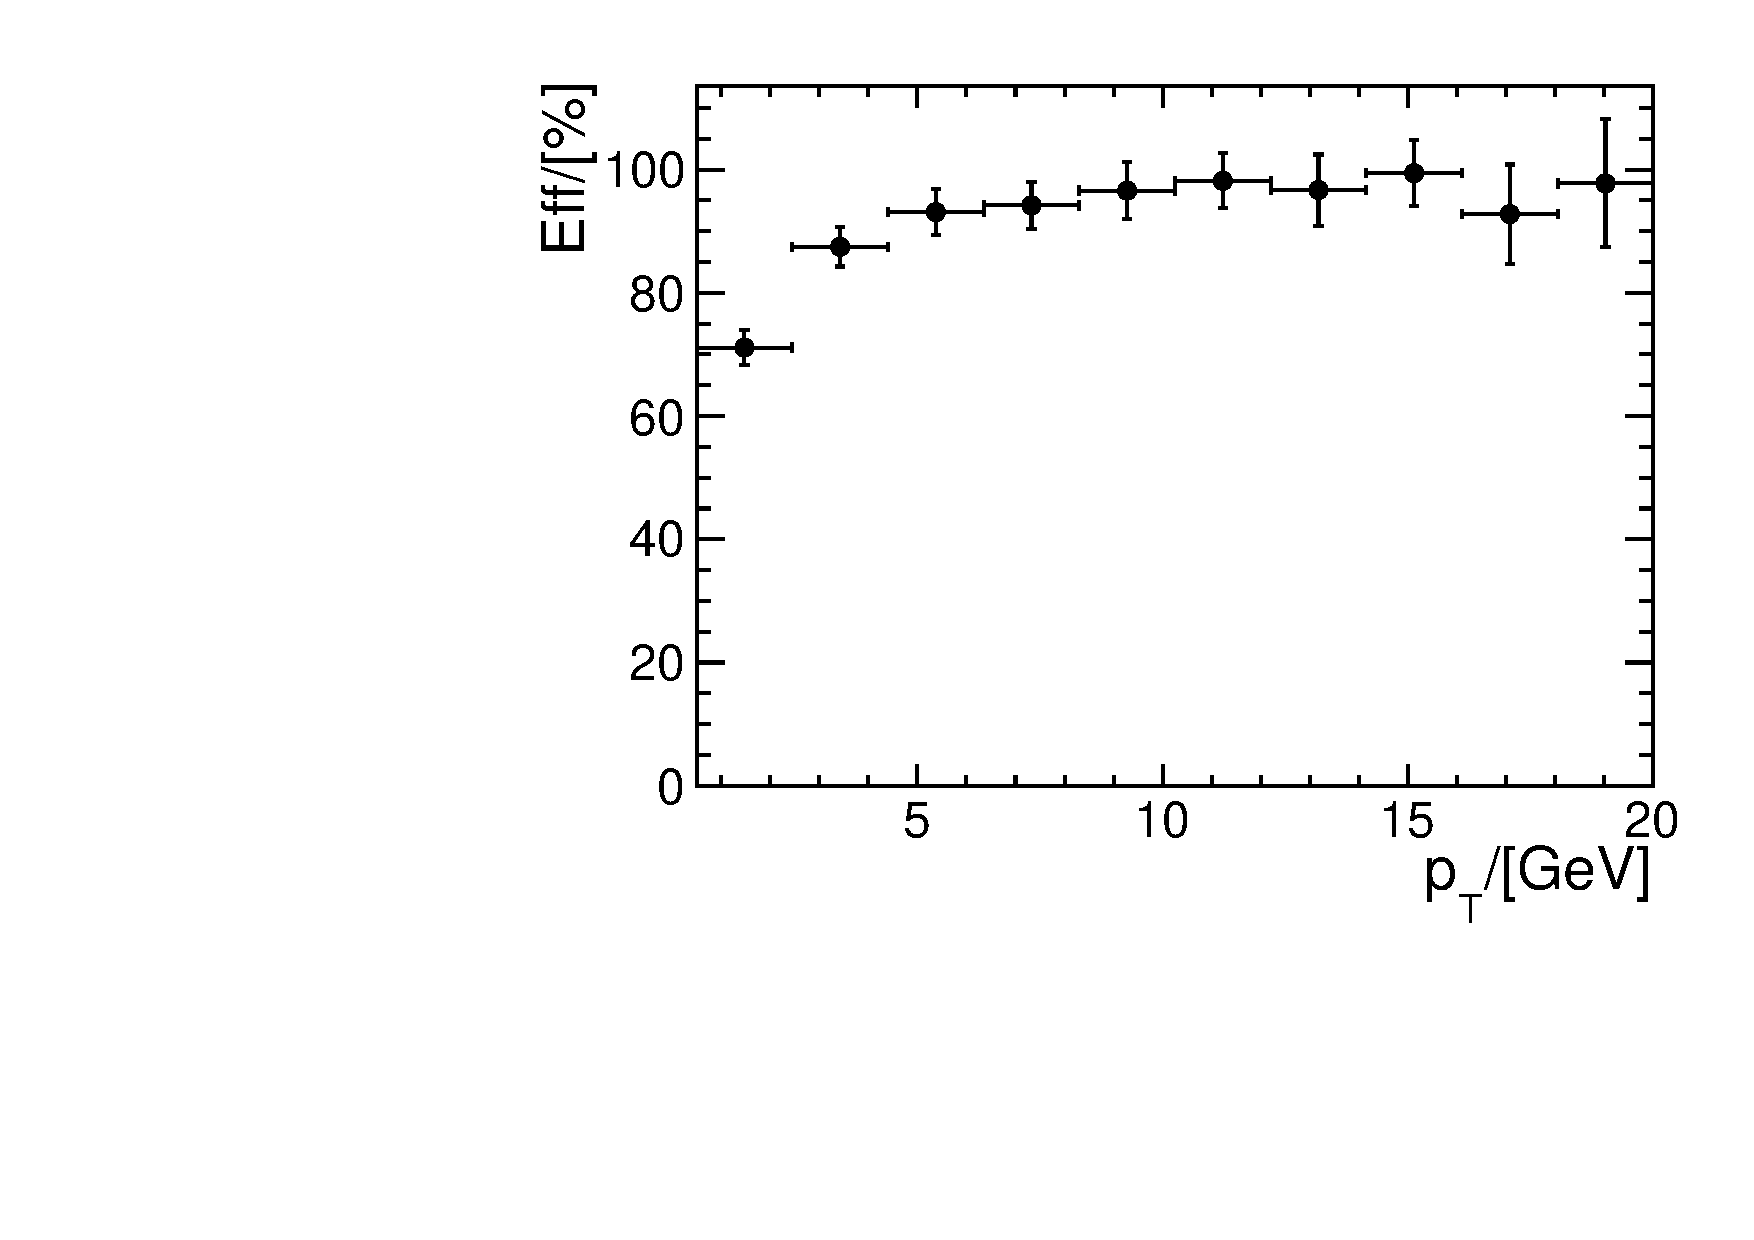
\includegraphics[width=0.45\textwidth]{Figures/06_ECAL/pi0_plots/new_eff.pdf}
%\caption{The \piz($E(\piz)<100\gev$) reconstruction efficiency with two $\gamma$ in \lhcb acceptance, 
%with $\pt(\gamma)>200\mev$.} 
%\label{fig:pi0_eff}
%\end{figure}
%
%\begin{figure}[!bp]
%\centering
%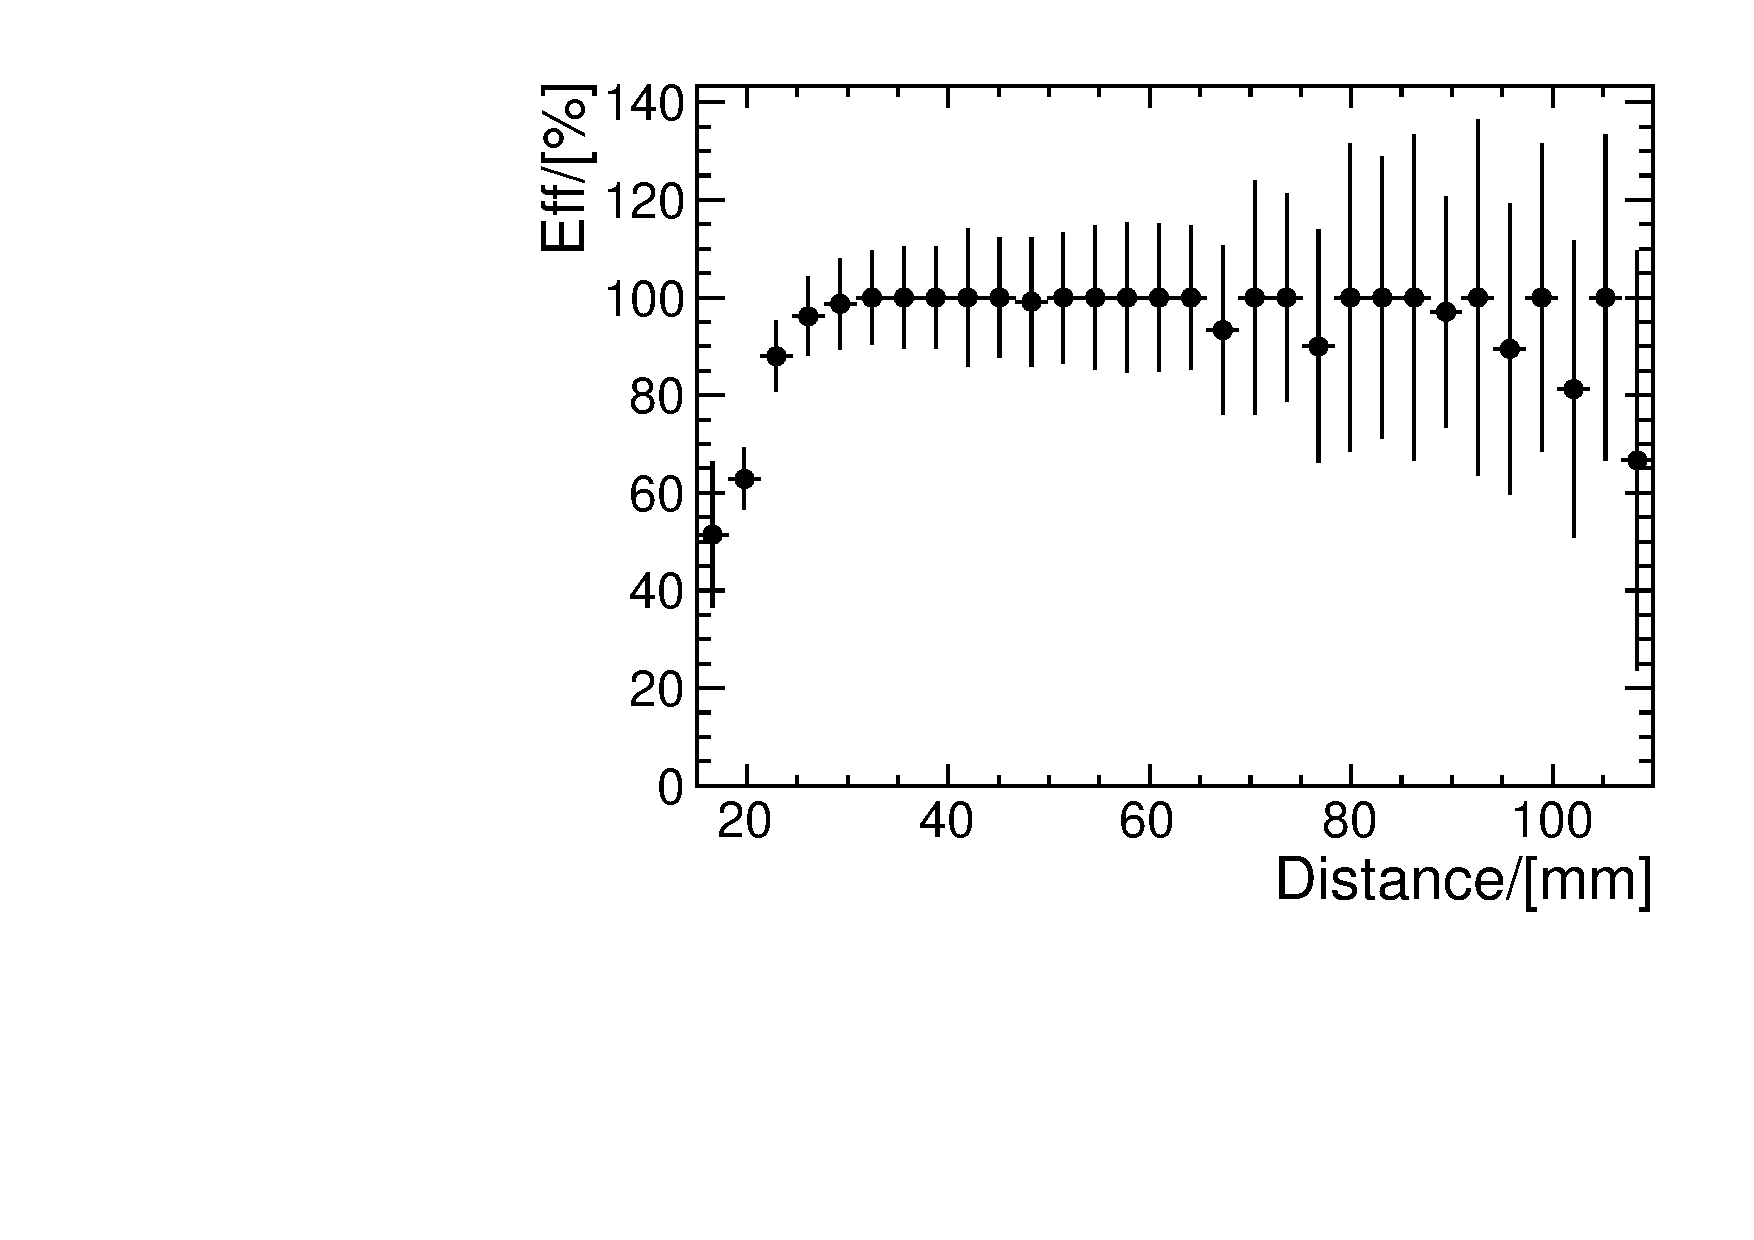
\includegraphics[width=0.45\textwidth]{Figures/06_ECAL/pi0_plots/distance_eff_20.pdf}
%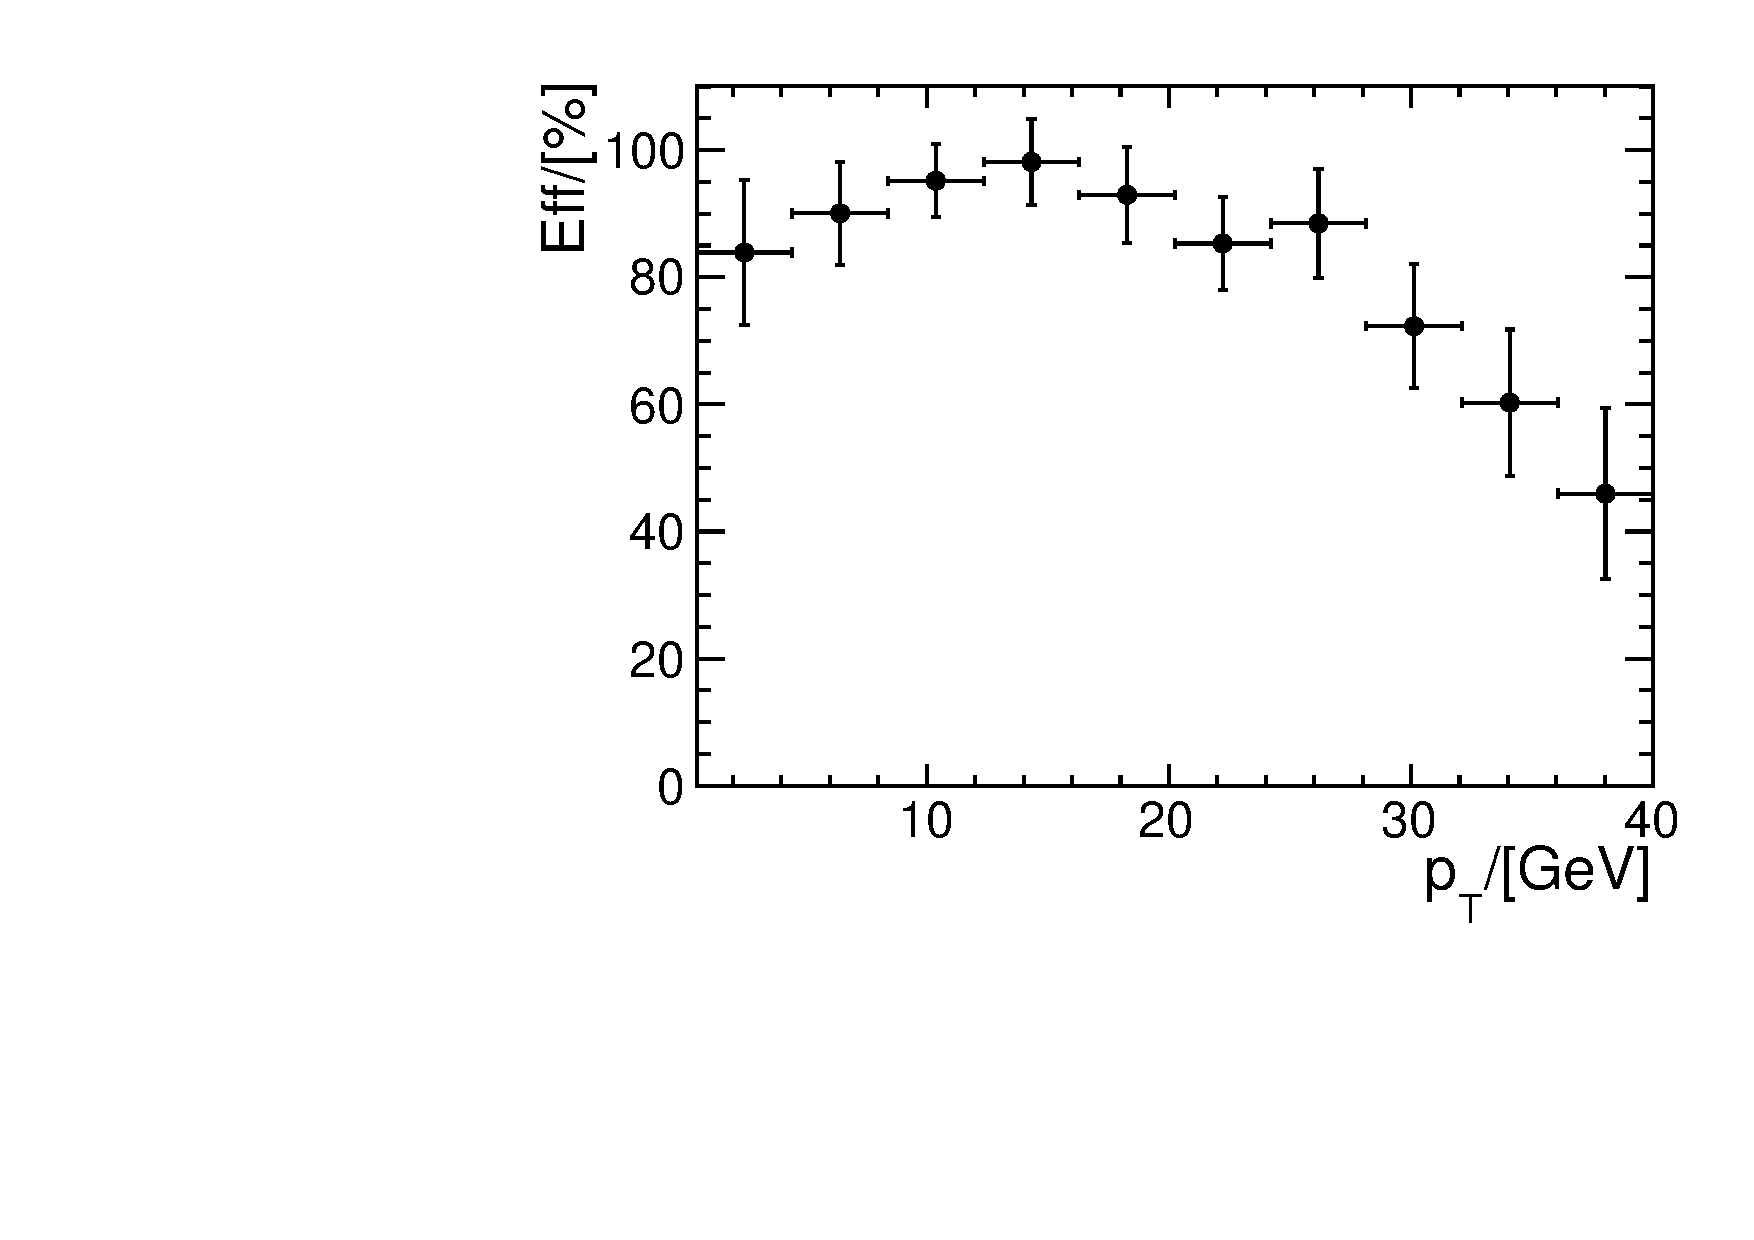
\includegraphics[width=0.45\textwidth]{Figures/06_ECAL/pi0_plots/new_eff_20.pdf}
%\caption{The \piz($E(\piz)<200\gev$) reconstruction efficiency with two $\gamma$ in \lhcb acceptance, 
%with $\pt(\gamma)>200\mev$.} 
%\label{fig:pi0_eff_200}
%\end{figure}
%
%In order to show the separation of the silicon-tungsten \ecal,
%the resolved \piz reconstruction efficiency with two $\gamma$ in \lhcb acceptance is studied.
%Figure.~\ref{fig:pi0_eff} shows the relation between the resolved \piz reconstruction efficiency and the distance of two $\gamma$ on the \ecal plane (left one), and  transverse momentum with the $E(\piz)<100\gev$ (right one).
%While the Figure.~\ref{fig:pi0_eff_200} shows the efficiencies with the $E(\piz)<200\gev$, 
%from this plots, 
%it is found that the resolved \piz reconstruction efficiency goes down when the distance of two $\gamma$ on the \ecal plane becomes smaller,
%which also means the energy \piz is larger according to Figure.~\ref{fig:pi0_distance_E}.
%
%Besides, 
%the variables to identifiy pure \g from merged \piz or ramdom overlapping cluster are also constructed,
%which have been introduced in the Section.~\ref{subsec:ecal_identification}.
%







